\documentclass[12pt, a4paper]{report}
\usepackage[utf8]{inputenc}
\usepackage[T1]{fontenc}
\usepackage{graphicx}
\usepackage{hyperref}
\usepackage{geometry}
\usepackage{amsmath}
\usepackage{amssymb}
\usepackage{booktabs}
\usepackage{caption}
\usepackage{xcolor}
\usepackage{tikz}
\usetikzlibrary{positioning, shapes.geometric, arrows.meta, fit, backgrounds, calc}

% ---------------------------------------------------------------------------
% Draft-only: highlights work still in progress, for the supervisors' first read.
%   \wip{status}                 -> box with a placeholder note
%   \wip[my comment]{status}     -> box with my own note
% To strip the styling for submission, replace the definition below with:
%   \newcommand{\wip}[2][]{#2}
% ---------------------------------------------------------------------------
\definecolor{wipframe}{RGB}{176,98,0}
\definecolor{wipbg}{RGB}{255,248,238}
\newcommand{\wip}[2][\emph{(comment to be added)}]{%
    \par\medskip\noindent
    \fcolorbox{wipframe}{wipbg}{%
        \begin{minipage}{\dimexpr\linewidth-2\fboxsep-2\fboxrule\relax}
            \textcolor{wipframe}{\textbf{Work in progress.}}\ #2\par
        \end{minipage}%
    }\par\medskip%
}
\geometry{a4paper, margin=1in}
\graphicspath{{figures/}}

\title{Assessing the Robustness of TerraMind to Sensor Domain Gap for On-board Processing on the $\Phi$-sat-2 Mission}
\author{Elouann Lucas \\ Copernicus Master in Digital Earth GeoData Track}
\date{\today}

\begin{document}

\begin{titlepage}
    \centering

    \vspace*{1cm}
    {\large Department of Geoinformatics, Faculty of Digital and Analytical Sciences\par}
    {\large Paris-Lodron Universität Salzburg\par}
    \vspace{0.5cm}
    {\large Faculté Sciences \& Sciences de l'Ingénieur\par}
    {\large Université Bretagne Sud\par}

    \vspace{2.5cm}
    {\huge\bfseries Assessing the Robustness of TerraMind to Sensor Domain Gap for On-board Processing on the $\Phi$-sat-2 Mission\par}

    \vspace{1cm}
    {\Large Master Thesis\par}

    \vspace{2.5cm}
    {\Large Elouann Lucas\par}
    \vspace{0.2cm}
    Copernicus Master in Digital Earth GeoData Track

    \vspace{2.5cm}
    {\large\bfseries Supervisors\par}
    \vspace{0.3cm}
    Assoc.\ Prof.\ Sébastien Lefèvre\\
    Nicolas Longépé, ESA Supervisor\\
    Assoc.\ Prof.\ Martin Sudmanns

    \vfill
    {\large \today\par}
\end{titlepage}

\begin{abstract}
On-board processing is a promising answer to the downlink latency and bandwidth constraints that limit the usefulness of Earth observation data for time-critical applications such as flood and wildfire response.
Geospatial Foundation Models (GeoFMs) are interesting candidates for this task, since their large-scale multimodal pre-training gives semantic feature extractors that generalize across tasks with few labeled examples.
However, these models are pre-trained on archived data from missions such as Sentinel-2, and their behaviour once they are exposed to a new sensor is not known.
This thesis studies three questions, with TerraMind, a Vision Transformer (ViT)-based GeoFM, and the European Space Agency's $\Phi$-sat-2 CubeSat mission as the case study: whether TerraMind produces domain-invariant latent representations on real $\Phi$-sat-2 imagery, whether a lightweight Convolutional Neural Network (CNN) distilled from it can be made sensor-adaptive, and whether doing so is actually better than simply training the compact model on the target sensor.

We use a co-registered triplet dataset of real $\Phi$-sat-2, real Sentinel-2 and physics-simulated $\Phi$-sat-2 imagery, which lets us measure the domain gap directly, as the distance in TerraMind's embedding space between two sensor views of the same ground.
The gap is already there in the early layers of the encoder, and a linear probe transfers only a third of its source-domain accuracy to the target sensor.
This points to a low-level, radiometric origin in the two sensors' differing spectral response functions, since a semantic cause would rather have surfaced in the deeper layers.
Plain fine-tuning on physics-degraded data does not close the gap either.
Domain-specific batch normalization, applied to the student during cross-architecture knowledge distillation into a lightweight CNN, does reduce it (cosine similarity $0.098 \rightarrow 0.948$, probe transfer $33\% \rightarrow 97\%$), and it only requires that the sensor of each input is known, which is always the case on board.
A paired-contrastive objective exploiting the co-registered pairing was also implemented and evaluated, but it did not do better than domain-specific normalization alone.
Whether this adaptation is worth adopting then depends on the label budget.
The distilled, domain-adapted student outperforms a supervised baseline of identical architecture trained directly on the target sensor at a representative labeled-data budget (mIoU $0.4532$ vs.\ $0.3989$), but it loses to that same baseline at a smaller one (mIoU $0.2679$ vs.\ $0.2916$).
A few-shot comparison against $\Phi$satNet, an on-orbit GeoFM developed for the same mission, is planned but remains to be run.

% What these results show is that a deliberate, domain-aware adaptation is necessary if GeoFMs are to generalize on board resource-constrained EO missions: an incidental exposure to degraded data does not deliver it, and the more complex paired mechanism is not required to. How much this adaptation is worth then depends on the label budget.

\end{abstract}

\tableofcontents
\newpage

\chapter{Introduction}
\label{chap:introduction}

Earth observation (EO) satellites now capture more data than ground segments can downlink and process in a timely manner\cite{barretta2026onboardaireview}.
Ground-based processing is adequate for most applications, but time-critical ones such as flood mapping\cite{tellman2021satellite} and wildfire detection\cite{taylor2013wildfire} require near real-time (NRT) inference, since the events they monitor can evolve within hours.
Moving the inference step from the ground to the satellite itself removes this constraint.
Instead of downlinking large raw imagery for later processing, an on-board model can downlink a small processed data product.
This paradigm shift overcomes the downlink bottleneck for time-critical applications, and a growing number of missions have begun demonstrating its technical feasibility\cite{barretta2026onboardaireview}.
The European Space Agency's $\Phi$-sat-2 mission is among the most complete demonstrations to date: a 6U CubeSat carrying an 8-band high-resolution multispectral imager alongside a space-qualified Intel Movidius Myriad 2 VPU (Vision Processing Unit)\cite{myriad2}.
Instead of running a single fixed application, $\Phi$-sat-2 uses the NanoSat MO Framework\cite{coelho2021phisat2} to install, update, and orchestrate multiple AI applications on board, much as a smartphone runs installable apps.

To date, applications that were created to run on board $\Phi$-sat-2 have been small, task-specific convolutional neural networks (CNNs), each trained, validated, and uplinked individually for a specific job such as cloud masking, vessel detection, or roadmap extraction\cite{marin2021phi}.
To add a new capability to the system, the entire pipeline needs to be repeated from scratch.
Geospatial Foundation Models (GeoFMs) offer a different model of development.
Pre-trained on large, diverse archives of EO imagery, a GeoFM such as TerraMind\cite{jakubik2025terramind} learns a general-purpose semantic representation that downstream tasks can exploit with comparatively few labeled examples, without requiring a bespoke architecture and a full training run per application.
This property matters specifically for applications like flood and burnt-area mapping, where labeled events are rare by nature and a mission cannot simply wait to accumulate a large annotated archive before it becomes useful in an emergency.

Two significant challenges stand between this promise and an operational on-board GeoFM.
The first is the architectural constraints due to target hardware limitations.
TerraMind is built on the Vision Transformers (ViTs)\cite{dosovitskiy2020image} architecture, which is structurally incompatible with space-qualified accelerators of the Myriad 2's generation\cite{myriad2}, as it predates the hardware and software support that ViT inference requires.
The second is the operational domain gap due to sensor differences.
GeoFMs such as TerraMind are pre-trained on Sentinel-2 and similar archived missions, but $\Phi$-sat-2 has a different sensor, and the properties of its imagery are different enough from Sentinel-2's such that the model might not generalize well to it, this phenomenon is known as a domain gap\cite{bendavid2010theory}.
Each problem has to be solved individually, as a compressed model built without addressing the domain gap simply compresses the gap with it, and a domain-adapted ViT still cannot run on the target hardware.

This thesis addresses both obstacles together, using TerraMind and $\Phi$-sat-2 as the case study, with flood segmentation as the motivating downstream application.
The methodological approach combines three elements.
First, a physics-based sensor degradation pipeline, based on the simulator developed for the ESA $\Phi$-lab OrbitalAI challenge\cite{longepe2024orbitalai}, is used to process Sentinel-2 imagery at the pixel level to simulate the $\Phi$-sat-2 sensor characteristics.
This simulation pipeline produces labeled training data for a target sensor that hasn't accumulated data for flood segmentation yet.
Second, a purpose-built dataset of spatially and temporally co-registered image triplets (real $\Phi$-sat-2, real Sentinel-2, and simulated $\Phi$-sat-2, all of the same scene) makes it possible to measure this domain gap directly in latent space and to test candidate adaptation mechanisms against it, instead of relying on downstream accuracy alone.
Third, domain-specific batch normalization is applied during knowledge distillation\cite{hinton2015distilling} of the TerraMind encoder into a lightweight CNN: the student keeps a separate set of normalization statistics per sensor on otherwise shared weights, so the deployable model adapts to whichever sensor it is actually reading from at inference, since that sensor identity is always known on board.
A paired-contrastive alignment objective exploiting the co-registered triplets directly was also implemented and evaluated as an alternative mechanism, but did not improve downstream task performance beyond what domain-specific normalization already provides.

\section{Problem Definition}
\label{sec:problem-definition}

The main technical problem is a covariate shift between the sensor domain a GeoFM is pre-trained on and the sensor domain it is tasked to operate on.
Let $X$ denote the space of satellite image patches and $Y$ the space of semantic labels (land-cover class, flood/background).
Writing $p_s$ and $p_t$ for the source (pre-training, e.g.\ Sentinel-2) and target (operational, e.g.\ $\Phi$-sat-2) distributions, a covariate shift is present when
\begin{equation}
    p_t(x) \neq p_s(x) \quad \text{while} \quad p_t(y \mid x) = p_s(y \mid x).
    \label{eq:covariate-shift}
\end{equation}
In practice, the physical scene and its semantic content are identical across the two domains, but the sensors produce different pixel statistics.
This shift occurs because of differing spectral response functions, point spread functions, signal-to-noise characteristics, and geometric band-to-band alignment, all of which are properties of the sensor rather than the scene itself.
A model whose learned representation is sensitive to these sensor-specific statistics instead of the underlying semantics will degrade on the target domain even though nothing about the task itself has changed.

Prior work on GeoFM domain gap has typically measured this shift only indirectly, through downstream task performance, and has compared source and target datasets that differ in geography, acquisition date, and scene content in addition to sensor, which confounds the sensor-specific shift this thesis is concerned with and the shift due to the underlying data distribution itself.
The co-registered triplet dataset used in this work is designed specifically to remove that confound, since the real $\Phi$-sat-2, real Sentinel-2, and simulated patches used for evaluation depict the same scene at the same time.

\section{Research Gap}
\label{sec:research-gap}

Two related works describe in similar ways the gap this thesis addresses.
Du et al.
\ \cite{du2025onorbitdemonstrationgeospatialfoundation} demonstrated an on-orbit GeoFM (compressed Prithvi) on the Kanyini CubeSat and the IMAGIN-e payload, adapting it to the target sensor by retraining task heads on a limited set of real target-domain labels while keeping the encoder frozen.
However, the domain gap they measure between source and target domains are from different benchmark datasets, not co-registered pairs, so sensor-induced shift is not isolated from content and geographic shift.

Within the $\Phi$-lab, a GeoFM named $\Phi$satNet was developed specifically for on-board execution on $\Phi$-sat-2 hardware. Based on the U-Net architecture (CNN-based), it avoids the ViT-compatibility problem by training from scratch on a pre-training methodology involving physics-simulated $\Phi$-sat-2 data.
Neither of these works isolate sensor-only covariate shift using co-registered data, and they don't test whether an existing GeoFM's broad, diverse pre-training transfers to a new sensor with fewer labels.
This thesis addresses the first of those directly; the second involves a matched label-efficiency comparison against $\Phi$satNet, which is framed but left to future work (Section~\ref{sec:discussion-comparison}).
The gap this thesis addresses is therefore threefold: (i) whether the domain gap between $\Phi$-sat-2 and Sentinel-2-pretrained TerraMind can be measured directly, in latent space, using data that isolates sensor-induced covariate shift; (ii) whether that gap can be closed through an explicit domain-adaptation mechanism; and (iii) whether the resulting adaptivity survives compression into a hardware-deployable, cross-architecture (ViT-to-CNN) student model.

\section{Research Objective and Problem Statement}
\label{sec:research-objective}

The objective of this thesis is to determine whether the representational benefits of a large-scale, Sentinel-2-pre-trained GeoFM can be carried across the sensor domain gap into a lightweight CNN that must operate on $\Phi$-sat-2 imagery and run on the $\Phi$-sat-2 on-board processor.
TerraMind is not itself adapted to $\Phi$-sat-2 so it is used as a frozen teacher on the Sentinel-2 domain it was pre-trained for. 
To bridge the gap, the student is trained on both domains and learns to generalize across sensors to be operated on one.
The question is therefore whether a student distilled under this arrangement represents the two sensors consistently and performs well on the target sensor, without giving up the advantage that motivated starting from a GeoFM instead of training from scratch.
This objective is pursued through three research questions:

\begin{enumerate}
    \item Does the domain gap caused by sensor differences between $\Phi$-sat-2 and Sentinel-2 measurably affect the latent representations produced by TerraMind, and if so, where in the encoder does this effect concentrate?
    \item Can a lightweight CNN distilled from TerraMind be made sensor-adaptive given that naive fine-tuning on degraded data alone does not achieve this, and which mechanism is actually responsible if so: domain-specific normalization, a paired-contrastive objective exploiting the co-registered triplets, or both?
    \item Does distilling from TerraMind in this way improve downstream $\Phi$-sat-2 task performance over simply training a compact model of the same architecture directly on the target sensor, so that sensor-adaptivity and task accuracy are assessed as two separate questions, without assuming the former implies the latter?
\end{enumerate}

Answering these questions would show that the generalization promise of large GeoFMs (broad semantic transfer from limited labels) is compatible with the low-latency, resource-constrained inference that on-board emergency-response applications require, provided the measured domain gap is addressed.

\chapter{Background and Literature Review}
\label{chap:background}

This chapter positions the thesis against five parts of the work that each contribute to the overall problem, which is to make the representational benefits of a GeoFM available on board a resource-constrained satellite.
Each part is treated in turn, before a closing synthesis states what combination of them remains unaddressed.

\section{On-board AI for Earth Observation}
\label{sec:onboard-ai}

The volume of data returned by Earth observation missions keeps growing, driven both by the number of platforms in orbit and by the increasing capability of their instruments, whether through finer spatial resolution or, in the hyperspectral case, far denser spectral sampling.
The result is a body of products that covers the globe repeatedly and serves a wide range of applications.
Extracting value from it means moving from observations to information, and ultimately to decisions taken by users who are not themselves remote sensing specialists.
Machine learning is well suited to automating that step, since it can interpret the complex, high-dimensional structure of EO acquisitions for tasks such as predictive analytics and anomaly detection\cite{barretta2026onboardaireview}.

The conventional way of applying such models keeps the whole inference stage on the ground.
Models are trained on datasets compiled from the archives of one or several missions, and each new acquisition is downlinked in full before any information is extracted from it.
This is the bent-pipe architecture (Figure~\ref{fig:workflow}), in which the satellite acts as a passive relay: it acquires data, applies at most minimal preprocessing, and transmits the result to a ground station without interpreting it\cite{razzano2024ai}.
The arrangement keeps mission design simple, but it makes the useful output of a mission dependent on ground infrastructure and bounds it by downlink bandwidth and latency, which is what prevents a near-real-time response.

\begin{figure}[htp]
    \centering
    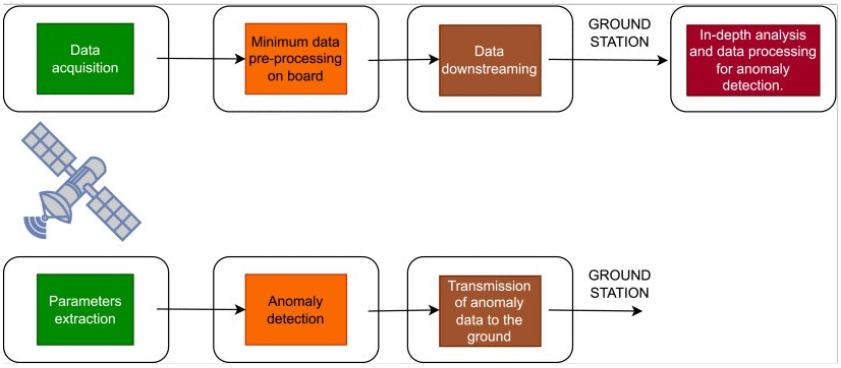
\includegraphics[width=12cm]{fig_onboard_workflow.png}
    \caption{Top Workflow (Bent-Pipe Architecture): Data is acquired and minimally preprocessed on the satellite before being transmitted to the ground station, where in-depth analysis for anomalies is conducted.
        Bottom Workflow: The satellite extracts parameters and detects anomalies onboard, transmitting only the relevant anomaly data to the ground station, reducing data transmission and enabling faster detection.
        From Razzano et al.~\cite{razzano2024ai}.
    }
    \label{fig:workflow}
\end{figure}

Because the satellite is not part of the information extraction process under this arrangement, and because modern missions add to an already large archive faster than it can be exploited, there is growing interest in running inference on board, on the imagery as the sensor captures it.
Not every platform can host such a model.
Image-processing networks, convolutional and deep neural networks in particular, are poorly matched to the processors typically flown, which are chosen for reliability and power efficiency instead of throughput, and offer limited computation and memory\cite{barretta2026onboardaireview}.
An AI-enabled satellite therefore carries a model uplinked from the ground and trained for that mission specifically.

$\Phi$-sat-1 was the first mission to demonstrate that this is achievable, running a cloud-detection network on board a hyperspectral imager and establishing on-board AI as a reliable and accurate tool for that task\cite{giuffrida2021phisat1}.
Two constraints shaped the result, with the first being the on-board hardware: dedicated processing had to be developed for the mission, operating within the platform's power budget and tolerating the faults that radiation induces in orbit.
The second is the lack of data as there wasn't enough imagery from the HyperScout product line existed to train a network to label every pixel as cloudy or clear, a recurring difficulty for space imagers, since a bespoke camera is generally developed for each new mission and its archive necessarily begins empty.
The network eventually deployed was a custom segmentation architecture designed around the accelerator's limits, and the bound on intra-layer memory in particular governed how its convolutional and deconvolutional layers could be implemented\cite{giuffrida2020cloudscout}.

CNN-based models of this kind are efficient, but their locality leaves them less able to capture the long-range patterns and contextual dependencies that more demanding remote sensing tasks require.
ViT architectures have become popular in computer vision due to their ability to capture global context via self-attention mechanisms, often outperforming CNNs on a variety of tasks\cite{han2022survey}.
This makes ViT-based models strong candidates for on-board EO applications, and in a comparative study of ViT variants for onboard satellite image classification Le et al.~\cite{le2024onboard} report that pre-trained ViTs consistently outperform equivalent models trained from scratch.
These pre-trained models also require lower computational cost, and are more resilient to noise, which is close to the combination an on-board setting needs the most.
Their cost nonetheless remains the primary barrier to deployment, since the large parameter counts and the attention computation that give ViTs their advantage are precisely what a resource-constrained satellite can least afford\cite{chou2023edge}.
The hardware on board $\Phi$-sat-2 is a constraining factor for the deployment of models, as the CogniSAT-XE1 payload is equipped with the Intel Movidius Myriad 2 VPU~\cite{myriad2}.
The support for this hardware has been discontinued in 2020, which makes it legacy.
The $\Phi$satNet effort reports that the most recent OpenVINO release supporting this hardware is version 2020.3, that experimental testing confirmed only ONNX opset 8--11 are available\footnote{Supported operations are listed here: \url{https://docs.openvino.ai/2023.3/openvino_docs_ops_opset11.html}}, and that the resulting lack of dynamic-axes support renders transformer-based architectures such as ViT incompatible with the target~\cite{phisatnet}.
These constraints, documented in detail by the $\Phi$satNet effort, are the main motivations for cross-architecture distillation, in place of direct deployment or same-family compression.

\section{Geospatial Foundation Models}

Foundation models are a class of large, pre-trained neural networks that can be adapted to many downstream tasks with minimal additional training\cite{bommasani2021opportunities}.
This paradigm has been widely adopted in natural language processing and computer vision, where models such as BERT, GPT, and CLIP have demonstrated remarkable performance across a range of tasks.
These models are characterized by their pre-training strategy, which typically involves self-supervised learning on massive, diverse datasets, and by their ability to generalize across tasks and domains.
Once a foundation model is pre-trained, it can be fine-tuned on specific tasks, which makes them highly versatile and efficient for a wide range of applications.

GeoFMs\cite{lu2025vision} extend the foundation-model paradigm from natural images to Earth observation.
Pre-training gives a single large backbone of diverse, multi-modal EO archives so that many downstream tasks can be solved by fine-tuning a small task-specific head instead of training a full model from scratch.
TerraMind\cite{jakubik2025terramind} is a ViT-based, multimodal GeoFM pre-trained on the multimodal TerraMesh dataset\cite{blumenstiel2025terramesh}, which includes Sentinel-2 data.
It is explicitly designed to produce transferable semantic representations rather than task-specific features.
However, that capacity has, to date, mostly been demonstrated on data drawn from the same sensor family the model was pre-trained on, leaving open how it behaves under different sensor conditions.

\section{Domain Gap}
\label{sec:domain-gap}

A domain gap is a distribution shift between the data a model was trained on and the data it must work with once deployed.
Because a learned model only holds where the distribution it was fitted to holds, such a shift generally shows up as a loss of accuracy, and it does so even when nothing about the task itself has changed.
The problem is acute for on-board AI, where the model is fixed at uplink time while acquisitions continue to vary with illumination, atmosphere, season, geography, and the behaviour of the instrument itself.
It is useful to separate three kinds of shift, since they have different causes and admit different remedies\cite{kouw2019introductiondomainadaptationtransfer}.

\begin{itemize}
    \item[--] \emph{Covariate shift} is a change in the distribution of the inputs while the labelling rule stays the same: the same scene content is represented differently, for instance because the imagery carries blur, sensor noise, or haze that the training data did not.
    \item[--] \emph{Prior shift} is a change in the distribution of the labels themselves, as when a class that is well represented in the source domain is rare or absent in the target, so a model calibrated on the source over-predicts it.
    \item[--] \emph{Concept shift} is a change in what a given label looks like: a forest in Brittany and a tropical forest in Vietnam carry the same land-cover label while containing different species with different spectral signatures, so the mapping from label to appearance is no longer the one the model learned.
\end{itemize}

This thesis is concerned with covariate shift, and specifically with the part of it attributable to the instrument.
The three kinds are difficult to separate in practice, because two datasets acquired by different sensors normally also differ in where and when they were acquired, and therefore in class balance and in scene content: a measured drop in accuracy then confounds all three.
The co-registered triplets described in Chapter~\ref{chap:methodology} are constructed to remove that confound.
Because each triplet holds views of the same ground at very nearly the same time, the label distribution and the underlying scene are held fixed across the pair by construction, leaving the sensor as the only factor that varies and the shift it induces as the only one being measured.

\subsection{Domain Adaptation}
\label{sec:domain-adaptation}

Domain adaptation (DA) addresses the general problem of a model trained on a source distribution being applied to a target distribution with different input statistics but unchanged semantics\cite{kouw2019introductiondomainadaptationtransfer}.
Within satellite on-board AI specifically, Du et al.
\ \cite{du2024domainadaptation} demonstrated DA for satellite-borne cloud detection by retraining task heads on real, though limited, labeled imagery from the Kanyini mission, with the encoder frozen.
This line of work was extended on-orbit by Du et al.
\ \cite{du2025onorbitdemonstrationgeospatialfoundation}, who deployed a compressed Prithvi-family GeoFM on Kanyini and the IMAGIN-e payload, adapting via real-label head retraining instead of encoder-level DA.
The domain gap is measured only indirectly through downstream task performance on source and target benchmark datasets that differ in geography and content as well as sensor.
This is the central limitation this thesis's data design addresses, because without co-registered source/target pairs of the same scene, a measured performance drop cannot distinguish sensor-induced covariate shift from confounding differences in what the two datasets depict.

Beyond retraining task heads, approaches to close the gap fall into a small number of families.
Their shared theoretical motivation is the bound of Ben-David et al.~\cite{bendavid2010theory}, which limits target-domain error by the sum of the source-domain error, a divergence between the two marginal input distributions, and a term for the error of the best joint hypothesis.
Since the first and third terms are not reduced by adaptation, the families below differ mainly in how they attack the divergence term.
Discrepancy-based methods penalize a statistical distance between the source and target feature distributions directly, most commonly the maximum mean discrepancy (MMD)~\cite{gretton2012kernel}, which requires only that samples from each domain is available.
Alignment-based methods make the stronger assumption that corresponding inputs are available, and pull their representations together explicitly.
X-STARS~\cite{marsocci2025cross} is the closest known example to the setting of this thesis: it adapts a model pre-trained on one optical sensor to a second sensor through a multi-sensor alignment dense loss, a patch-wise contrastive objective applied between paired acquisitions of the same area by both sensors, within a continual-pretraining framework.
It establishes that a paired-contrastive objective is effective when the sensor change is primarily one of spatial resolution, which is not the regime this thesis operates in: the $\Phi$-sat-2/Sentinel-2 gap measured in Chapter~\ref{chap:results-discussion} is driven mainly by differing spectral response.

A separate line of domain-adaptation work sidesteps alignment losses entirely by giving the model domain-specific normalization statistics instead.
Domain-Specific Batch Normalization (DSBN) \cite{chang2019dsbn} keeps a single set of convolutional weights but a separate batch-normalization affine transform and running statistics per domain.
This only requires that the domain of each example is known.
This is a smaller requirement than the paired-contrastive or MMD loss objectives discussed above, and, unlike them, is directly applicable wherever the deployed sensor is known at inference.

\section{Physics-Based Sensor Degradation Simulation}

Because labeled data from a satellite sensor does not exist before the satellite is launched, and accumulates slowly afterward for rare events, physics-based simulation of a target sensor's characteristics from an existing labeled source (typically Sentinel-2) has become a standard tool for pre-mission model development\cite{segl2012eetes}\cite{segl2015s2etes}.
% Explain more details about other simulators and their characteristics, and how they compare to the one used in this thesis, to provide a comprehensive overview of the field.
The simulator developed for the ESA $\Phi$-lab OrbitalAI challenge\cite{longepe2024orbitalai} models this transformation as a sequence of physical operations in radiance space, calibrated against real flight data from related missions: spectral and spatial resampling to the target sensor's band configuration and ground sampling distance, band-to-band misalignment consistent with push-broom acquisition geometry, signal-to-noise degradation, and optical blur modeled through the sensor's modulation transfer function.
This simulator underlies both the degradation pipeline used in this thesis and, independently, the pre-training and benchmarking datasets used by $\Phi$satNet (Section~\ref{sec:phisatnet-background}), making it shared, validated infrastructure within this research context that neither work claims as its own contribution.

\section{Knowledge Distillation Across Architectures}

Knowledge distillation (KD)\cite{hinton2015distilling} compresses a large "teacher" model into a smaller "student" by training the student to reproduce the teacher's output distribution.
By transferring the teacher's semantic knowledge (SK), KD allows the student to generalize better on large datasets with a lower computational cost.
Some feature-based variants exist that utilize the intermediate representations of the teacher, instead of training the student only against hard labels\cite{heo2019comprehensive}.
Le et al.~\cite{le2025semantic} proposed a distillation method between a ViT teacher and a ResNet student for image classification, which uses a dynamic weighting mechanism to adjust each teacher's influence on the student based on the teacher's confidence in its predictions.
Cross-architecture distillation is a necessary step here, since ViT inference is not supported on the $\Phi$-sat-2 on-board hardware (Section~\ref{sec:onboard-ai}).
On top of it, this thesis gives the student itself a domain-adaptation mechanism (domain-specific batch normalization, Section~\ref{sec:kd}).
This mechanism ensures that the student can learn domain-specific characteristics instead of relying on passive inheritance of whatever invariance the teacher might have been able to learn.
A paired-contrastive alignment objective exploiting the co-registered triplets was implemented and evaluated as an additional mechanism on top of this, but was found not to improve downstream task performance beyond what domain-specific normalization already provides (Section~\ref{sec:da-mechanism}).

\section{$\Phi$satNet}
\label{sec:phisatnet-background}

$\Phi$satNet is a U-Net-derived, multi-task-pretrained GeoFM being developed by the $\Phi$-lab specifically for on-board execution on $\Phi$-sat-2, using a purpose-built pre-training corpus and benchmark suite built on the same OrbitalAI simulator described above.
By training a compact, non-transformer architecture from scratch, $\Phi$satNet avoids the ViT-hardware-incompatibility problem entirely, and its authors report that it matches or exceeds unconstrained transformer-based GeoFMs on several on-board tasks~\cite{phisatnet}.
This is a different design philosophy from the one pursued here.
$\Phi$satNet optimizes for a hardware-native architecture trained on a curated, mission-specific task suite, while this thesis asks whether an existing, diversely pre-trained GeoFM can be adapted to new tasks with fewer labels than training a mission-specific model requires.

One property of $\Phi$satNet bears directly on the problem this thesis addresses.
Its pre-training method and its $n$-shot benchmarks are built entirely on simulated $\Phi$-sat-2 imagery derived from Sentinel-2, not on real acquisitions~\cite{phisatnet}.
$\Phi$satNet therefore does not escape the sensor domain gap by being mission-specific; it relocates it.
Its reported few-shot advantage rests on the assumption that physically simulated imagery stands in adequately for the real sensor, and its own evidence base, being simulated throughout, cannot test that assumption.
The sim-to-real question is thus one that the bespoke and the adapted approach inherit alike, and co-registered real acquisitions are what either would need in order to answer it.
A matched few-shot comparison against $\Phi$satNet on a shared task and label budget remains the appropriate test of the label-efficiency claim; Chapter~\ref{chap:results-discussion} returns to this positioning, but that comparison has not been run and is left to future work.

\section{Synthesis}

No work cited above isolates sensor-induced covariate shift using co-registered source/target data.
This thesis gives a cross-architecture distillation student an explicit, domain-aware adaptation mechanism, and verifies that this adaptivity, not only task accuracy, survives compression into hardware-deployable form.
The spatially and temporally co-registered $\Phi$-sat-2/Sentinel-2/simulated triplet dataset used in this thesis is what makes that isolation possible; the domain-specific batch normalization applied during cross-architecture distillation (Chapter~\ref{chap:methodology}) is what makes the adaptation and its verification possible.
The co-registered triplets serve, in addition, as the diagnostic instrument that shows a paired-contrastive alternative does not do better than the simpler domain-specific normalization.
The real-acquisition component also separates this work from the mission-specific alternative: $\Phi$satNet is pre-trained and benchmarked on simulated $\Phi$-sat-2 imagery, so the assumption that simulation stands in for the real sensor is one both approaches make and only real, co-registered data can check.

\chapter{Methodology}
\label{chap:methodology}

This chapter presents the complete analytical workflow: the data used and the role each dataset plays, the physics-based degradation pipeline and its calibration, the protocol for measuring the domain gap, the domain-adaptation mechanism adopted, the cross-architecture distillation procedure, and the evaluation protocol.
It closes with a dedicated account of the tooling and reproducibility practices used throughout.

The data underlying this work is split into two categories.
The first is the co-registered triplet dataset itself: real $\Phi$-sat-2 acquisitions, obtained via the ESA Insula Perception platform, matched to concurrent Sentinel-2 scenes and to a physics-simulated $\Phi$-sat-2 rendering of the same Sentinel-2 scene, co-registered using the LightGlue deep feature-matching algorithm \cite{Lindenberger_2023_ICCV} and filtered for spatio-temporal proximity and cloud cover.
This dataset carries land-cover labels derived from ESA WorldCover 2021, providing the only currently available real-sensor ground truth.
The second category is simulated: a physics-degraded, graded version of the Sen1Floods flood-segmentation benchmark, produced with the same degradation pipeline, standing in for a real labeled $\Phi$-sat-2 flood dataset that does not yet exist because the mission has not captured an annotated flood event.

The overall workflow followed a prototyping-implementation-refinement logic rather than a fixed plan executed once.
An initial conceptual model (fine-tune TerraMind on real $\Phi$-sat-2 labels, measure the gap, close it) was implemented, evaluated against intermediate diagnostics (embedding visualizations, similarity metrics), and revised twice on the basis of what those diagnostics showed: first when a normalization defect was found to be corrupting an early performance baseline (Section~\ref{sec:normalization}), and second when a first domain-adaptation mechanism was found, empirically, not to work (Section~\ref{sec:da-negative-result}), motivating the mechanism actually adopted (Section~\ref{sec:contrastive-mechanism}).

\section{Data}
\label{sec:data}

\subsection{The co-registered triplet dataset}
\label{sec:triplets}

The main dataset is a collection of spatially and temporally co-registered image triplets, produced in collaboration with the ESA $\Phi$-lab: real $\Phi$-sat-2 acquisitions (obtained via the ESA Insula Perception platform), the corresponding real Sentinel-2B scene, and a physics-simulated $\Phi$-sat-2 rendering of that same Sentinel-2 scene (Section~\ref{sec:degradation-pipeline}).
Candidate scenes were filtered by spatio-temporal proximity between the $\Phi$-sat-2 and Sentinel-2 overpasses and by a cloud-cover threshold on both acquisitions, and precise pixel-level alignment was achieved using the LightGlue deep feature-matching algorithm \cite{Lindenberger_2023_ICCV}, which identifies corresponding semantic keypoints across the two sensors despite their differing spatial and radiometric characteristics.

The choice of Sentinel-2 as the paired source sensor follows from the two instruments' band layouts.
Figure~\ref{fig:srf} compares their spectral response functions and their per-band spatial resolutions.
Across 400--900\,nm each $\Phi$-sat-2 multispectral band has a Sentinel-2 counterpart at a comparable centre wavelength, and it is that correspondence which makes Sentinel-2 usable both as the paired view in the triplets and as the source the degradation pipeline (Section~\ref{sec:degradation-pipeline}) projects into the $\Phi$-sat-2 domain.
The correspondence is close but not exact and $\Phi$-sat-2 additionally carries a panchromatic band with no Sentinel-2 equivalent.
Spatially, $\Phi$-sat-2 samples every band at a uniform 4.75\,m, whereas Sentinel-2 provides 10\,m for B2, B3, B4 and B8 and 20\,m for B5, B6 and B7.
The spatial resolution mismatch is a factor taken into account when interpreting the domain gap in Chapter~\ref{chap:results-discussion}: the target sensor is the finer of the two, so a resolution mismatch cannot by itself account for a loss of performance on $\Phi$-sat-2, whereas the spectral differences visible in panel~(a) remain a candidate explanation.

\begin{figure}[htp]
    \centering
    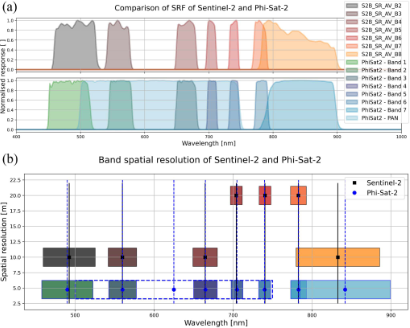
\includegraphics[width=12cm]{fig_srf_s2_phisat2.png}
    \caption{Band correspondence between Sentinel-2B and $\Phi$-sat-2, after Long\'ep\'e et al.~\cite{longepe2024orbitalai}.
        (a) Normalized spectral response functions, Sentinel-2B above and $\Phi$-sat-2 below.
        (b) Per-band spatial resolution.
        The correspondence in (a) makes Sentinel-2 usable as the paired source; the residual differences in both panels are the sensor gap this thesis aims to measure.
    }
    \label{fig:srf}
\end{figure}

This dataset carries labels for a single task: land-use/land-cover (LULC) classification, derived from ESA WorldCover 2021 and rasterized onto each triplet's real-$\Phi$-sat-2 footprint.
Its role in this thesis is twofold: it is the only real-sensor ground truth available for any downstream task, and its co-registration is what makes it possible to measure sensor-induced covariate shift in TerraMind's latent space (Section~\ref{sec:gap-measurement}) without the scene-content and geography confounds present in prior domain-gap studies that compare unrelated source and target datasets.

\begin{figure}[htp]
    \centering
    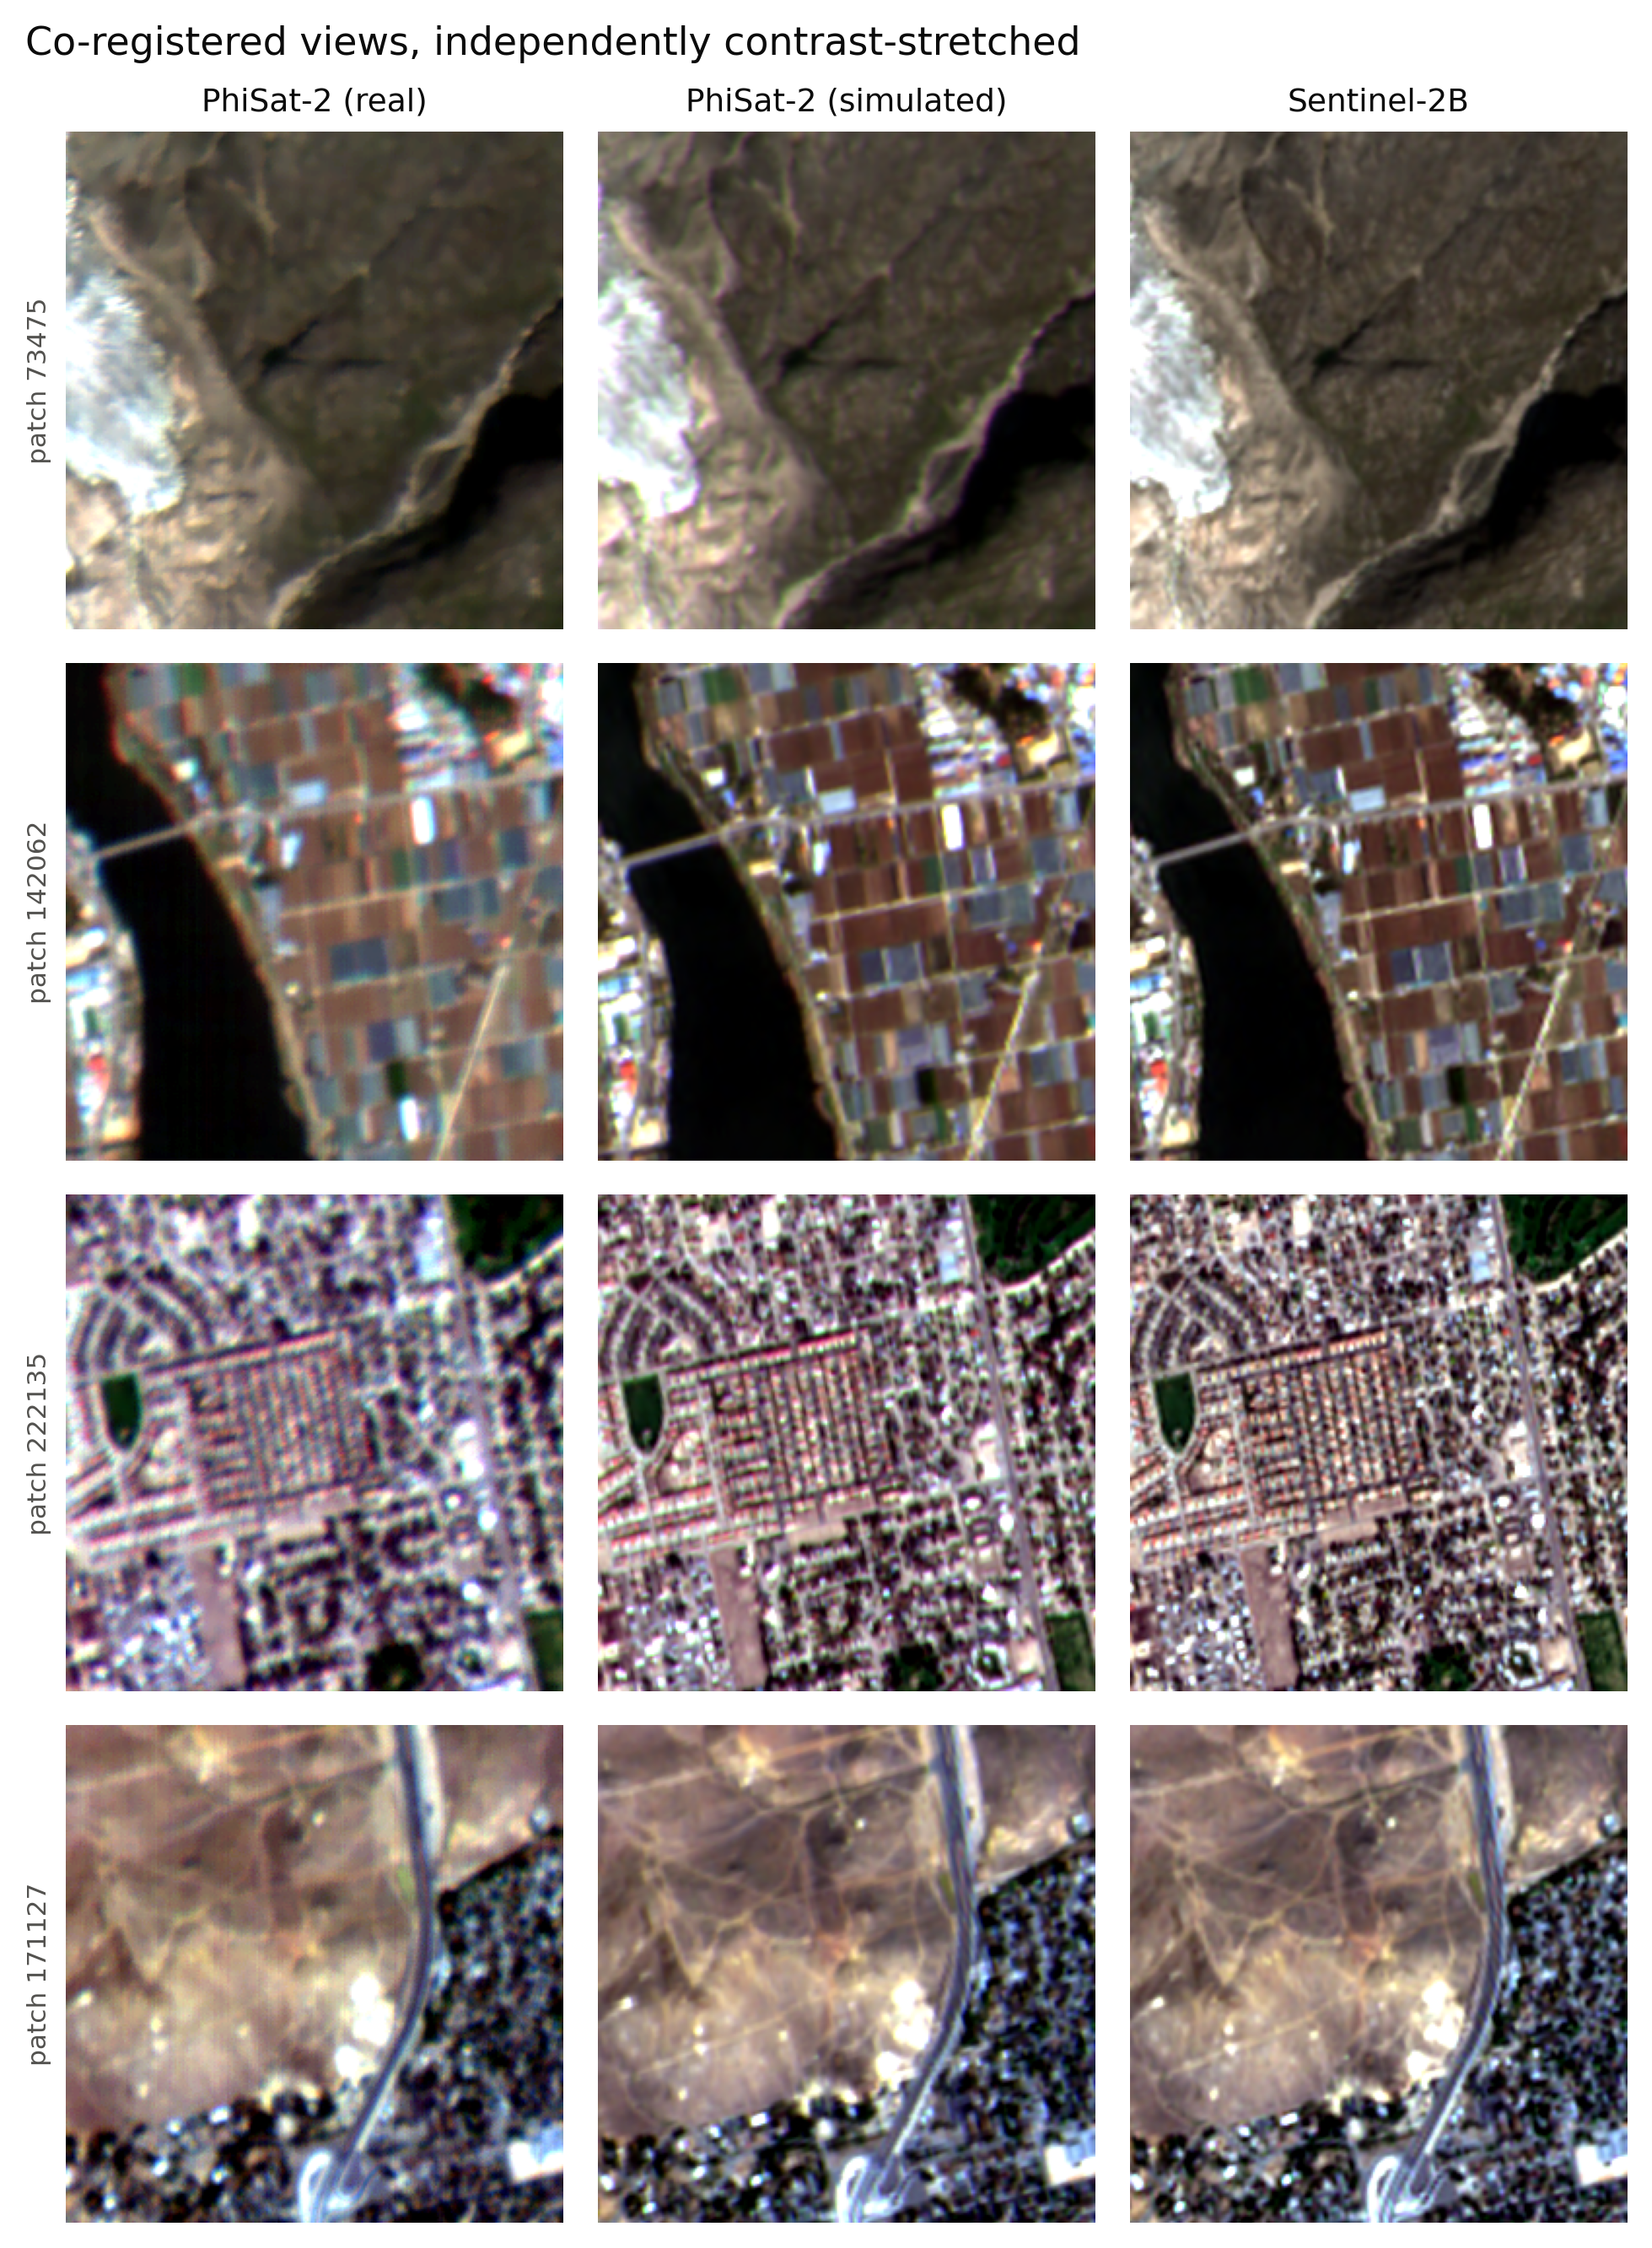
\includegraphics[width=12cm]{fig_patch_examples.png}
    \caption{Four representative triplets, each row showing the same scene as observed by real $\Phi$-sat-2, the physics-simulated $\Phi$-sat-2 rendering, and Sentinel-2B (each channel independently contrast-stretched for display).
        The real acquisitions show visibly grainier, noisier texture than either the simulated or source Sentinel-2 view, most apparent in the dark water/shadow region of patch 171127, consistent with the sensor noise characteristics the degradation pipeline (Section~\ref{sec:degradation-pipeline}) is designed to reproduce.
    }
    \label{fig:patch-examples}
\end{figure}

Figure~\ref{fig:patch-examples} shows four such triplets.
Qualitatively, the real acquisitions are consistently grainier than their simulated or source counterparts, and occasionally differ subtly in overall tone; the simulated column is, by construction, closer in appearance to Sentinel-2 than to the real sensor it is meant to approximate, a point returned to below.

\subsubsection{Scale and coverage}

After discarding a small number of corrupted source products, the dataset comprises 253{,}228 co-registered triplet patches drawn from 1{,}299 distinct $\Phi$-sat-2 products (individual acquisitions), a median of 209 patches per product (up to 713 for the largest).
Acquisitions span 2024-08-21 to 2026-04-15 (21 months), with collection volume markedly higher from mid-2025 onward than in the initial ramp-up period.
Real-$\Phi$-sat-2 and Sentinel-2 acquisition dates are matched to within a median of 6.8 days and a maximum of 14.9 days, not simultaneously, which is an acceptable temporal offset for a largely stable target such as land cover but a caveat worth stating rather than assuming away.
73.1\% of retained patches have under 5\% total cloud cover, and only 0.199\% of pixels are unlabelled after the ESA WorldCover rasterization step.

\begin{figure}[htp]
    \centering
    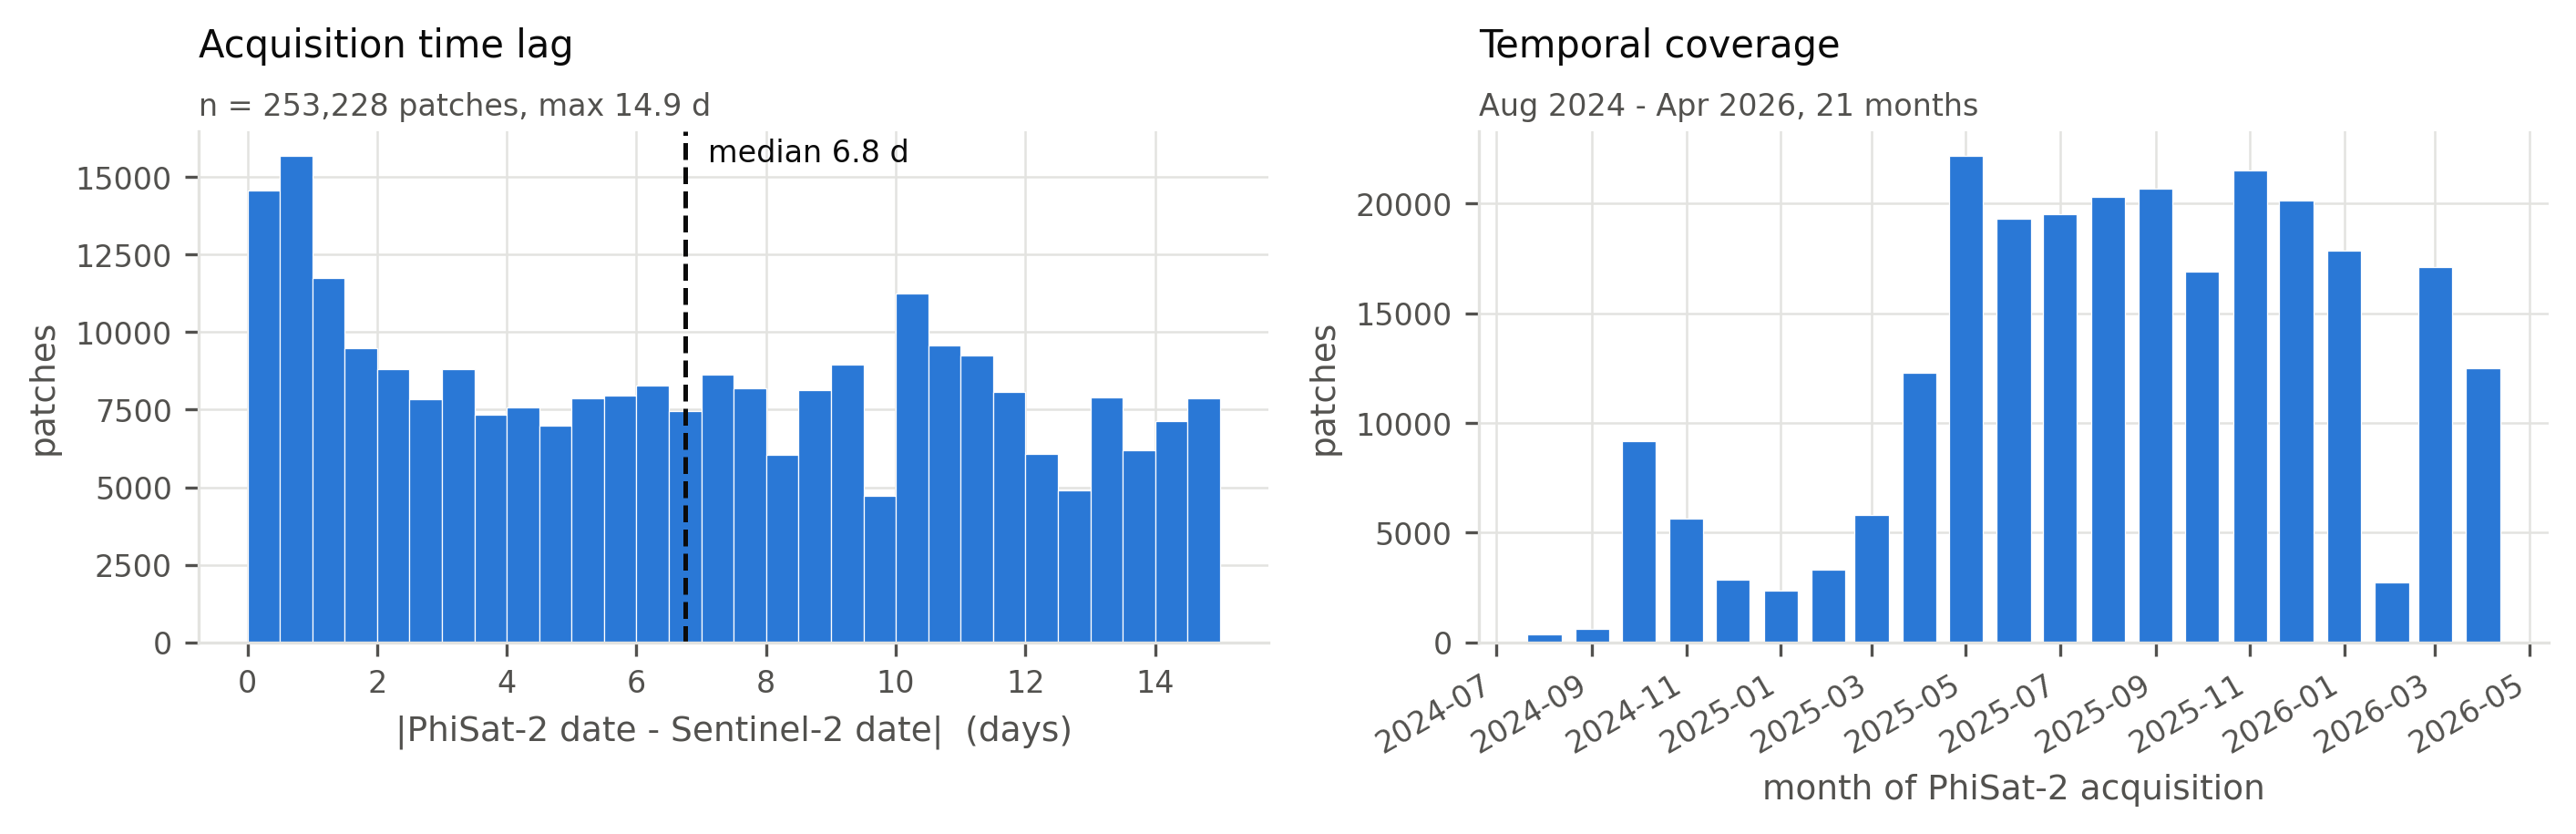
\includegraphics[width=\textwidth]{fig_acquisition.png}
    \caption{Left: distribution of the absolute time lag between matched $\Phi$-sat-2 and Sentinel-2 acquisitions (median 6.8 days, maximum 14.9 days, $n=253{,}228$).
    Right: monthly acquisition volume, Aug.
    \ 2024--Apr.\ 2026, showing the collection ramp-up in the first eight months.}
    \label{fig:acquisition}
\end{figure}

Geographically, the 1{,}299 source products span latitudes $-54^{\circ}$ to $76^{\circ}$ with global but uneven coverage, concentrated over western North America, the southern Andes, the Mediterranean basin and Middle East, and parts of East and South Asia (Figure~\ref{fig:geography}).
By K\"oppen--Geiger climate group, the patch population is dominated by arid (41\%) and temperate (29\%) climates, with tropical (14\%), continental (10\%), and polar (1\%) regions comparatively under-represented (4\% unclassified).

\begin{figure}[htp]
    \centering
    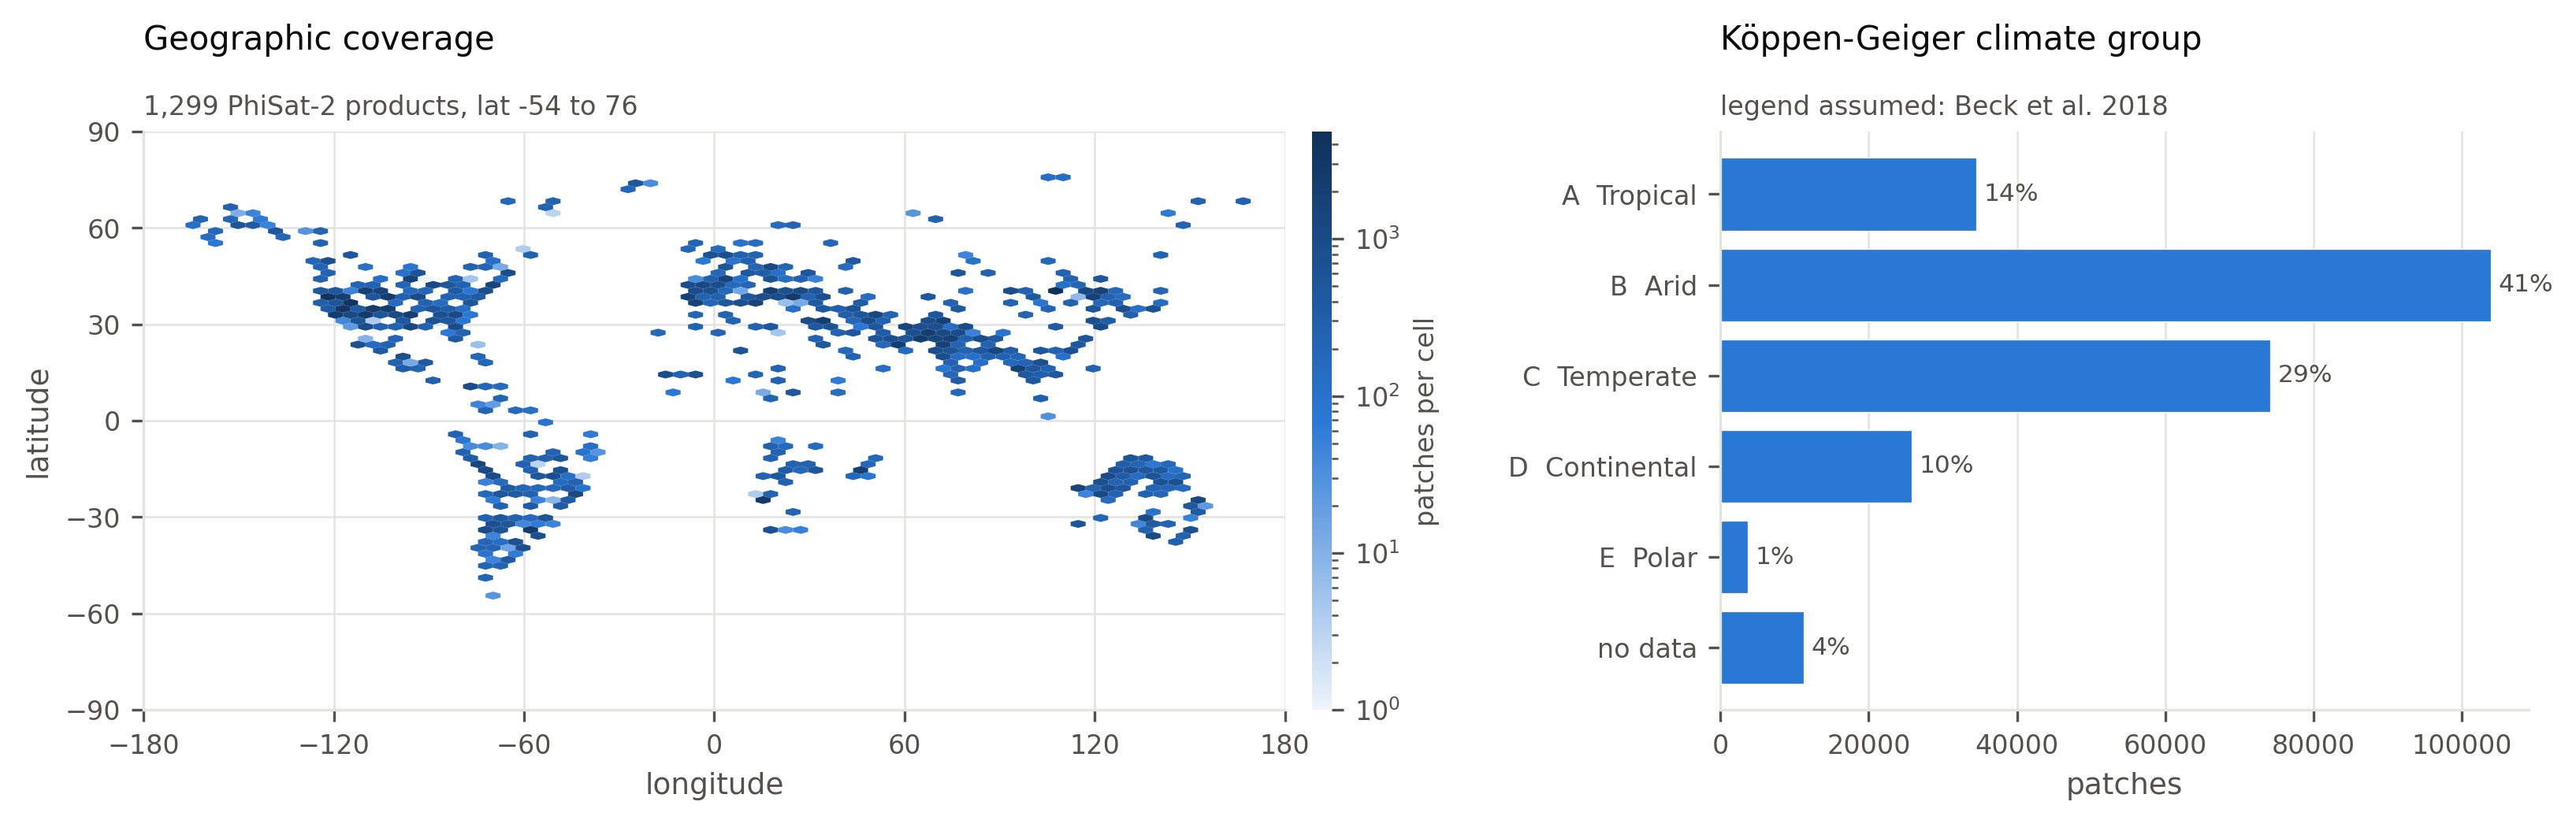
\includegraphics[width=\textwidth]{fig_geography.png}
    \caption{Left: spatial density of $\Phi$-sat-2 products (hexbin, log-scaled patch count per cell).
        Right: distribution of patches by K\"oppen--Geiger climate group\cite{beck2018present}.
    }
    \label{fig:geography}
\end{figure}

The eleven ESA WorldCover classes present are similarly imbalanced by construction rather than by sampling choice: grassland (20.8\%), tree cover (20.0\%), bare/sparse vegetation (16.2\%), built-up (14.4\%), and cropland (13.4\%) account for the large majority of labelled pixels, while snow/ice, mangroves, and moss/lichen each fall below 0.6\% (Figure~\ref{fig:landcover}).
The typical patch is fairly homogeneous: a single class occupies a median of 73\% of any given patch's labelled area.

\begin{figure}[htp]
    \centering
    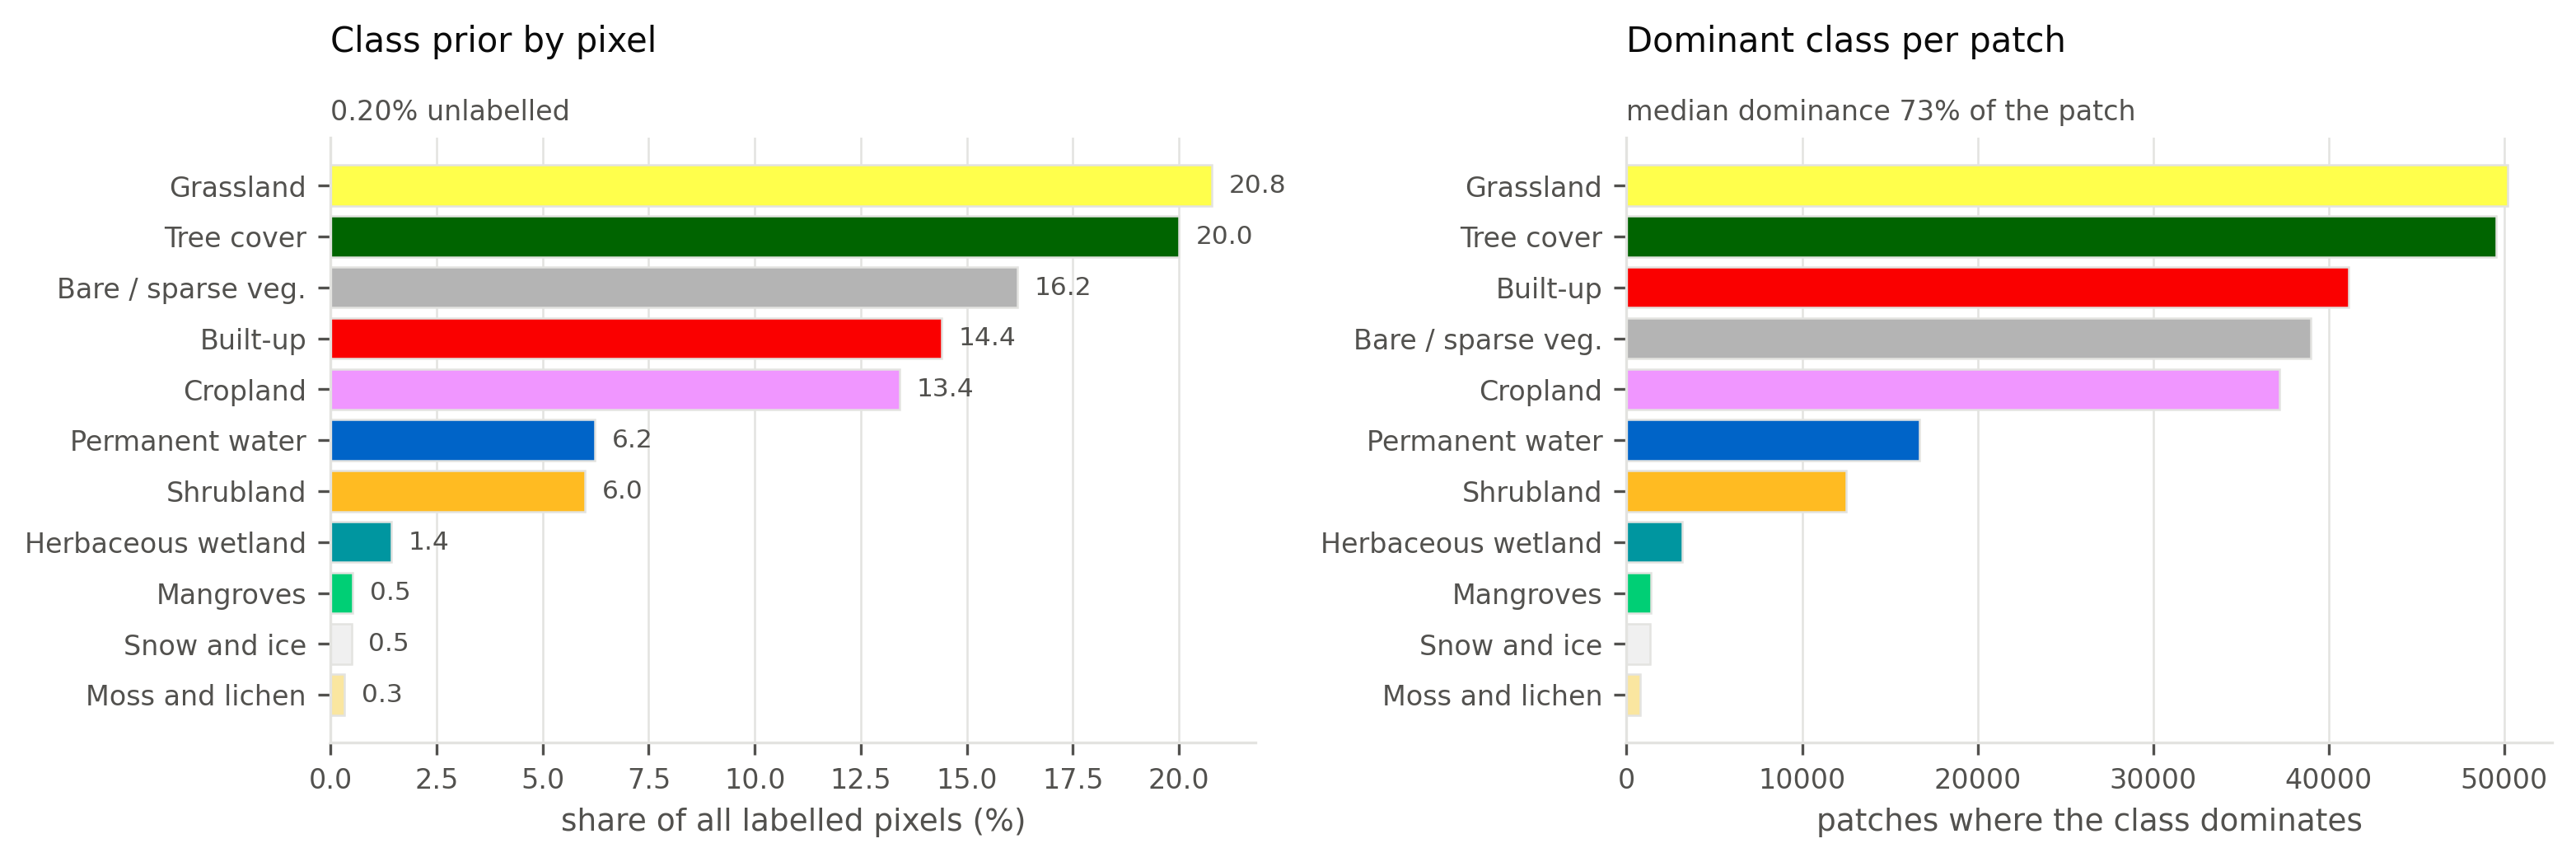
\includegraphics[width=\textwidth]{fig_landcover.png}
    \caption{Left: share of all labelled pixels by ESA WorldCover class.
        Right: number of patches in which each class is the dominant (plurality) class.
    }
    \label{fig:landcover}
\end{figure}

\subsubsection{Train/validation/test split}

The dataset is split 80/10/10 (202{,}582 / 25{,}323 / 25{,}323 patches) at the patch level with a fixed seed, and the resulting class-prior distribution is stable across all three splits, confirming the split does not introduce label-distribution shift (Figure~\ref{fig:splits}, left).
However this introduces a different problem, because splitting is patch-level rather than product-level, all 1{,}299 source products are represented in the training set, and every one of the 1{,}287 distinct products contributing to the test set also contributes patches to training (Figure~\ref{fig:splits}, right).
Since patches from the same product are spatially adjacent or overlapping crops of one acquisition, this means the test set is not a clean geographic or scene-level hold-out, and real-data performance figures reported in Chapter~\ref{chap:results-discussion} should be read as an optimistic upper bound on generalization to genuinely unseen scenes rather than as a strict out-of-sample estimate.
A product-level (rather than patch-level) re-split is the direct remedy and is noted as future work in Section~\ref{sec:discussion}.

\begin{figure}[htp]
    \centering
    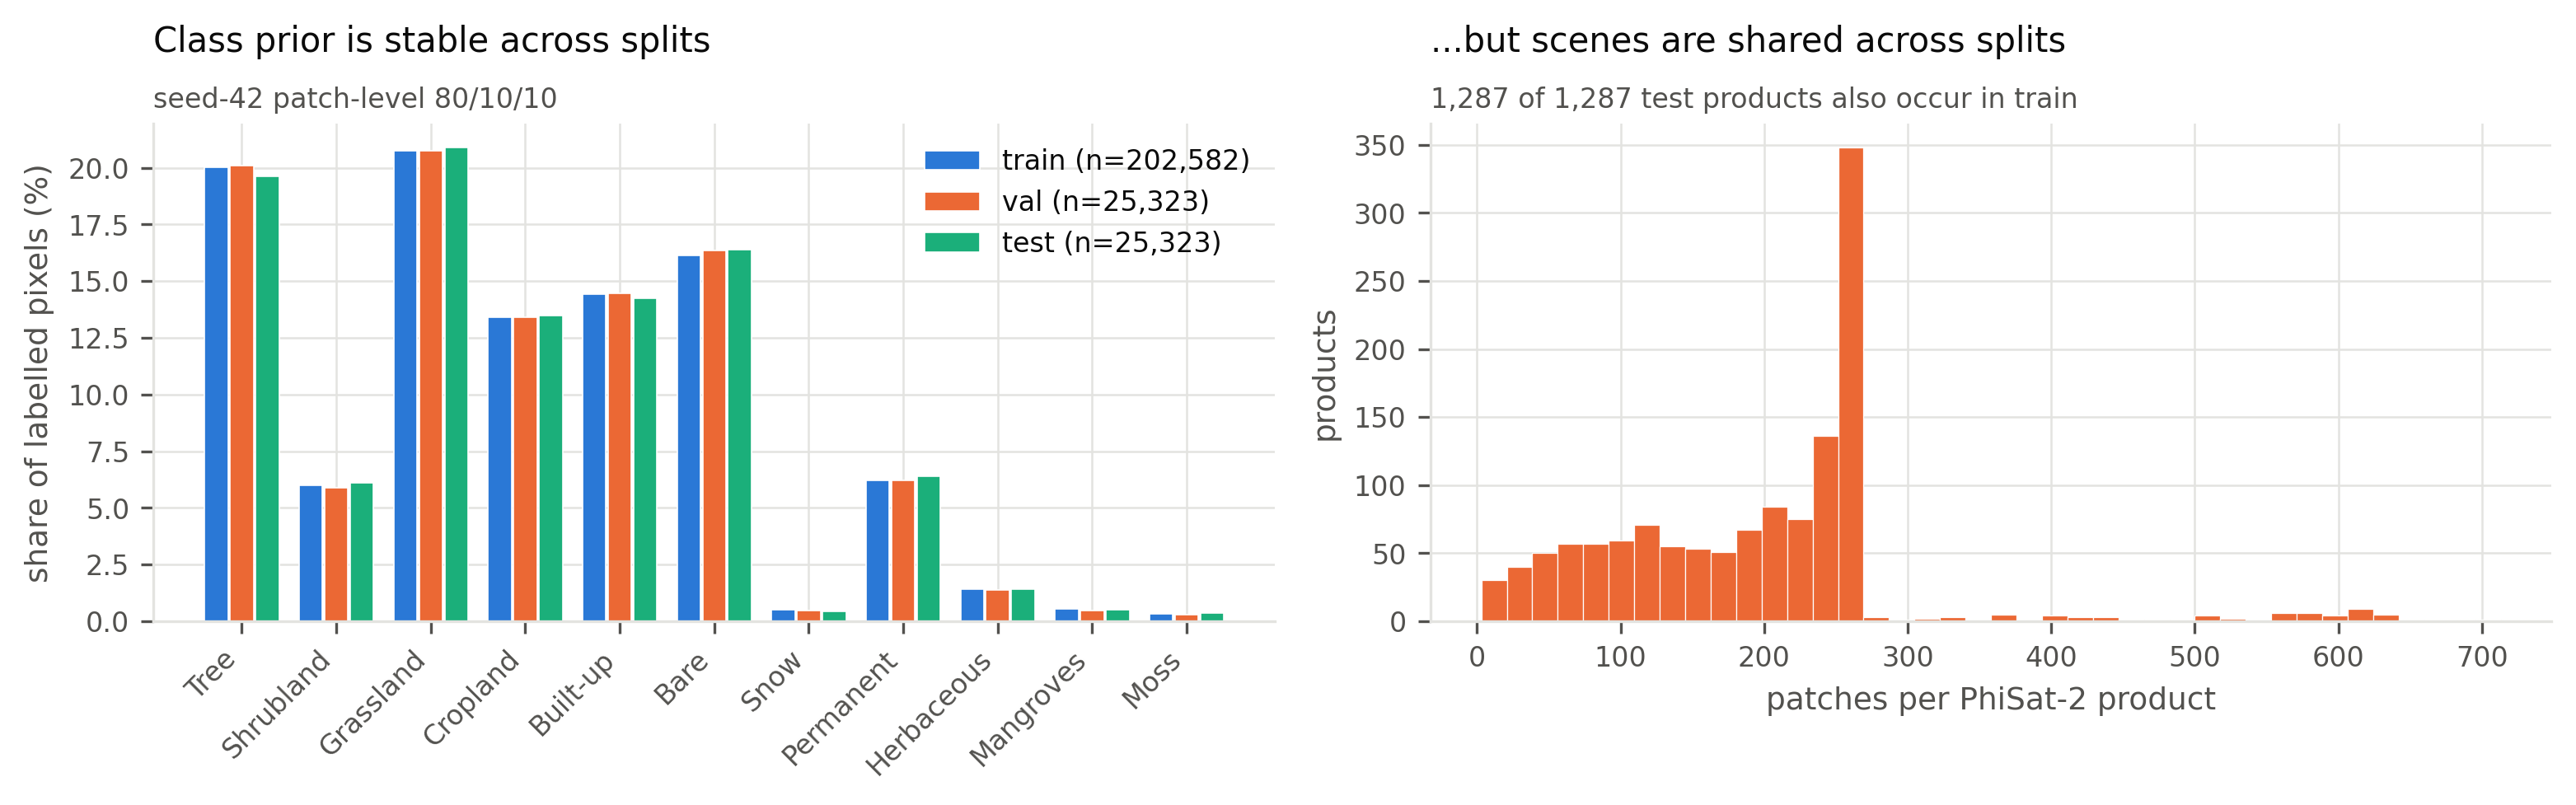
\includegraphics[width=\textwidth]{fig_splits.png}
    \caption{Left: class prior is stable across the train/validation/test split.
        Right: every one of the 1,287 products contributing to the test set also contributes patches to the training set: the split is patch-level, not scene-level.
    }
    \label{fig:splits}
\end{figure}

\subsubsection{Measured sensor discrepancy}

Three independent measurements quantify the sensor discrepancy this dataset is designed to expose, prior to any model being involved.

First, the raw radiometric scales of the two sensors heavily differ (Figure~\ref{fig:band-boxplots}): real $\Phi$-sat-2 digital numbers have per-band medians of about 55--150 (12-bit range, with measurable saturation of 2.1--2.2\% of pixels in the RE1/RE2 bands and dropout of 0.3--0.36\% in RE2/RE3), against Sentinel-2 and simulated-$\Phi$-sat-2 medians around 2{,}200--3{,}300, consistent with the Level-1C (L1C) Top-of-Atmosphere (TOA) reflectance-scaled DN convention.
The simulated and raw Sentinel-2 domains are close to statistically indistinguishable at this level (their boxes are overlapping in Figure~\ref{fig:band-boxplots}), confirming that the physics-based degradation pipeline (Section~\ref{sec:degradation-pipeline}) perturbs fine spatial and spectral structure rather than intensity statistics.
The domain gap this thesis is concerned with is therefore a real-vs-simulated gap, not a simulated-vs-source gap.

\begin{figure}[htp]
    \centering
    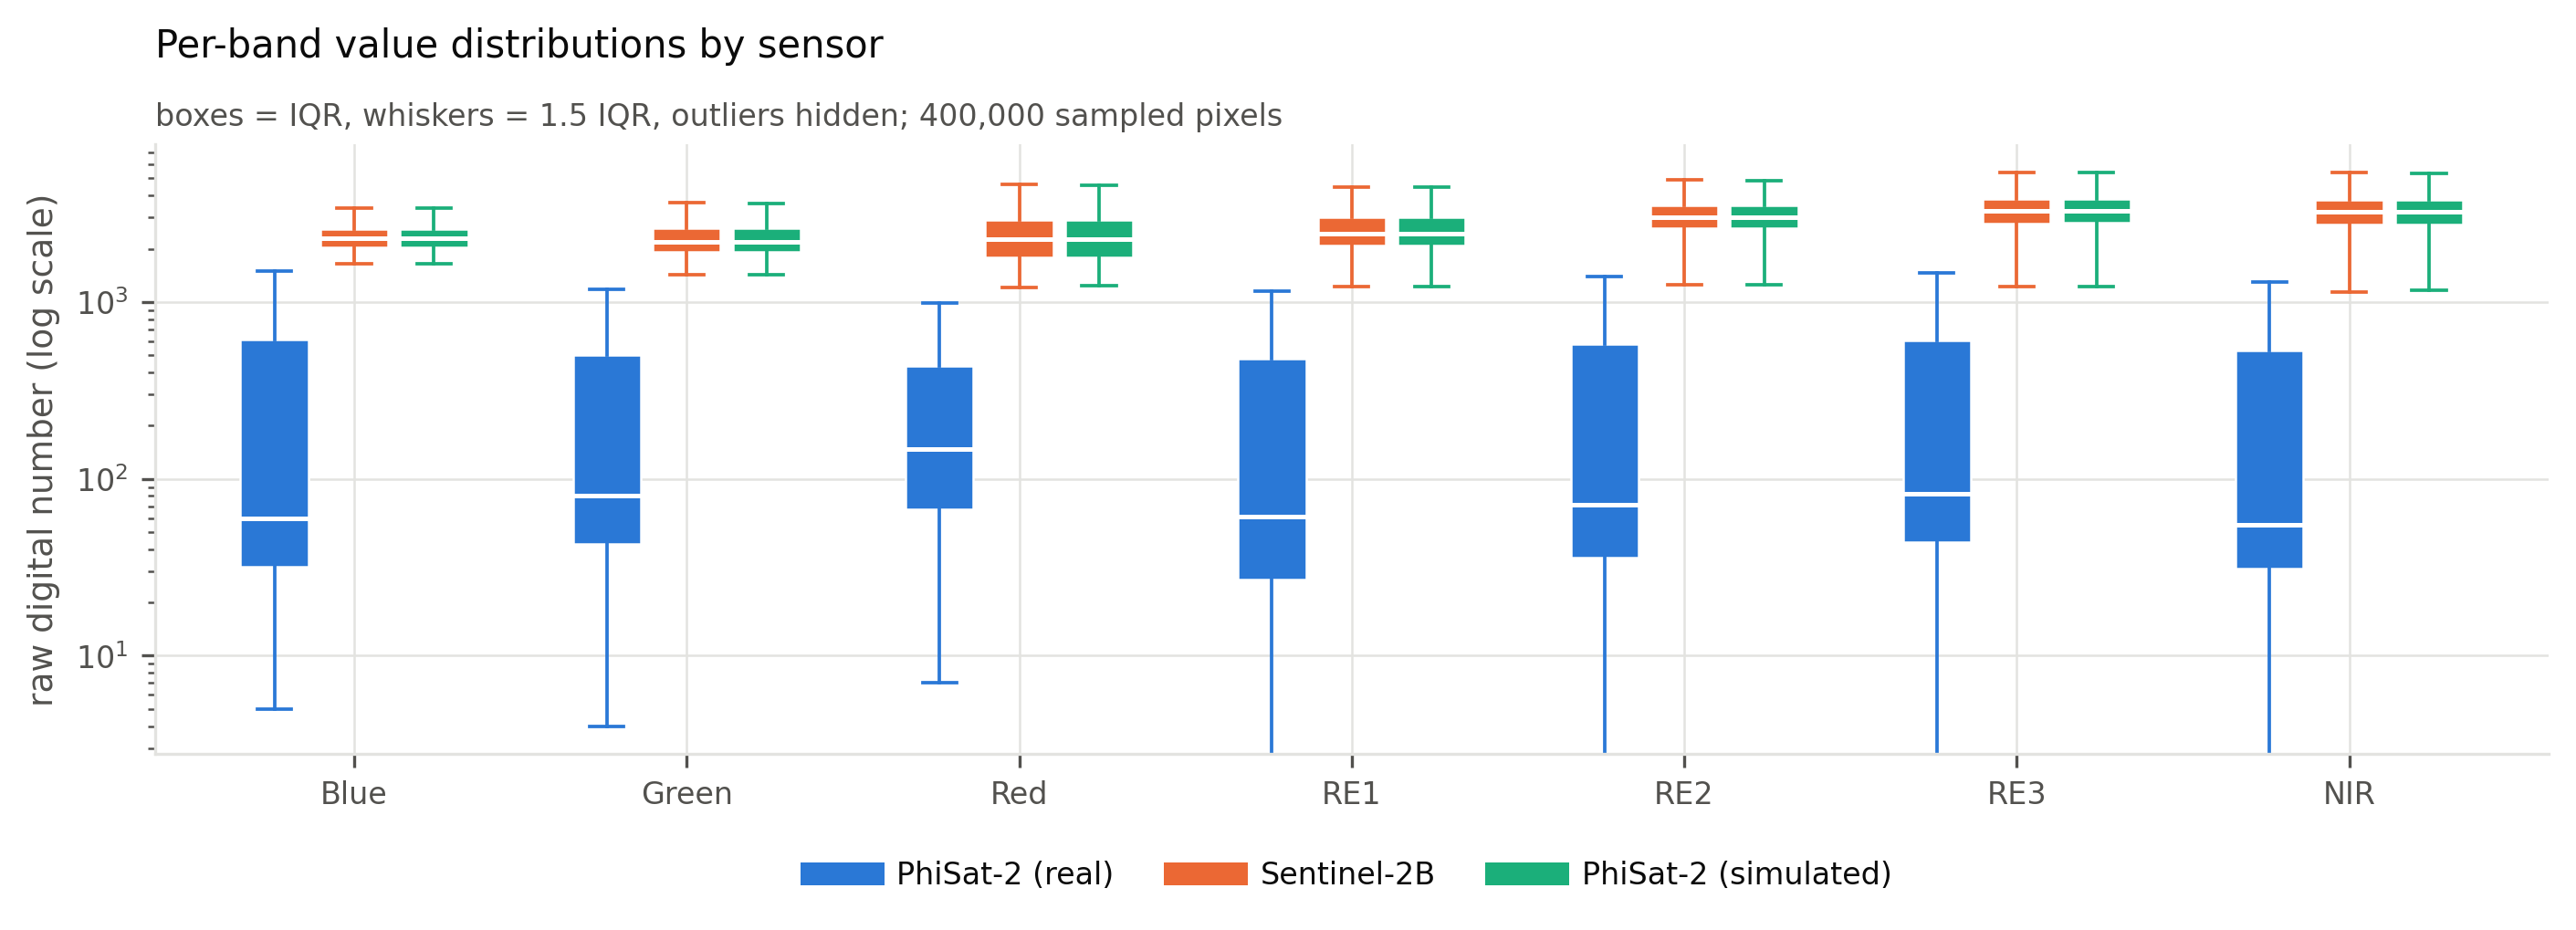
\includegraphics[width=\textwidth]{fig_band_boxplots.png}
    \caption{Per-band raw digital number distributions by sensor (log scale; boxes = IQR, whiskers = $1.5\times$IQR, outliers hidden; 400{,}000 sampled pixels).
        Real $\Phi$-sat-2 occupies a scale roughly one order of magnitude below Sentinel-2 and its simulated counterpart, which closely overlap each other.
    }
    \label{fig:band-boxplots}
\end{figure}

Per-domain normalization (Section~\ref{sec:normalization}) closes most, but not all, of this gap (Figure~\ref{fig:band-boxplots-normalized}): after $z$-scoring each sensor independently, the three distributions are centered similarly, but real $\Phi$-sat-2 retains visibly wider spread and longer tails in every band than Sentinel-2 or the simulated domain.
This residual spread difference, not the location/scale difference normalization already removes, is what the domain-adaptation mechanism of Section~\ref{sec:da-mechanism} must close.

\begin{figure}[htp]
    \centering
    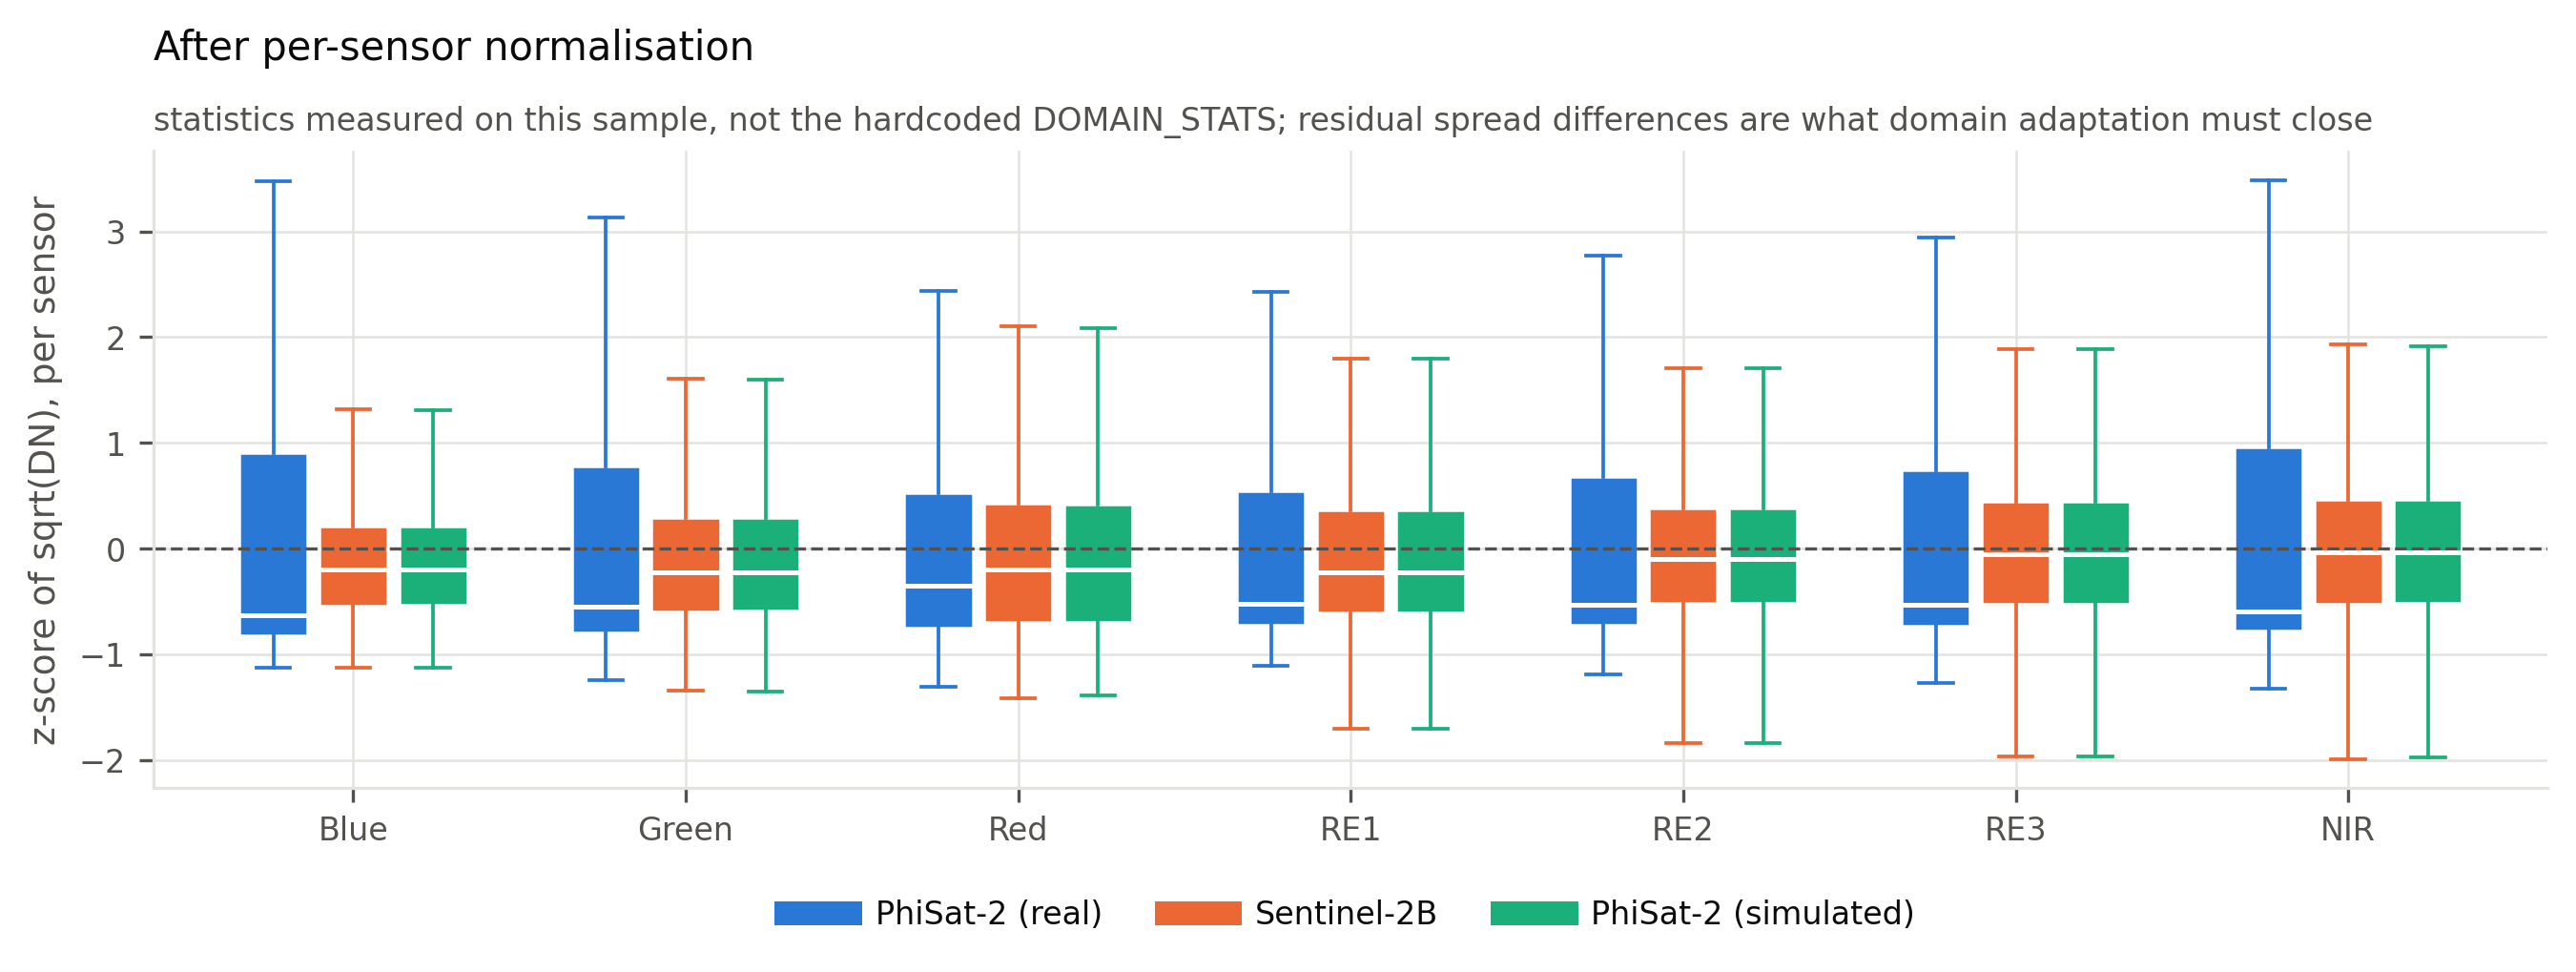
\includegraphics[width=\textwidth]{fig_band_boxplots_normalized.png}
    \caption{The same per-band distributions after per-sensor $z$-score normalization of $\sqrt{\text{DN}}$.
        Location and scale are aligned, but real $\Phi$-sat-2 retains a wider spread than Sentinel-2 or the simulated domain in every band: the residual gap normalization alone cannot close.
    }
    \label{fig:band-boxplots-normalized}
\end{figure}

Second, per-band correlation between co-registered real-$\Phi$-sat-2 and Sentinel-2 pixels is only weak-to-moderate even for matched same-scene observations (Pearson $r$ 0.31--0.54, Spearman $\rho$ 0.37--0.61 across the seven shared bands; Figure~\ref{fig:sensor-scatter}), with the weakest correspondence in the red-edge bands (RE1, RE2) and the strongest in the red band.
This is a direct, model-free demonstration that the two sensors disagree substantially about the same physical target observed within the same fortnight.
For contrast, the equivalent cross-band correlation between the simulated domain and its Sentinel-2 source is near-perfect (Spearman $\rho$ 0.98--1.00 on matching bands), as expected since the simulated patches are deterministic transformations of the same Sentinel-2 pixels.
The gap between real and simulated $\Phi$-sat-2 is therefore not explained by any weakness in the correlation analysis itself.

\begin{figure}[htp]
    \centering
    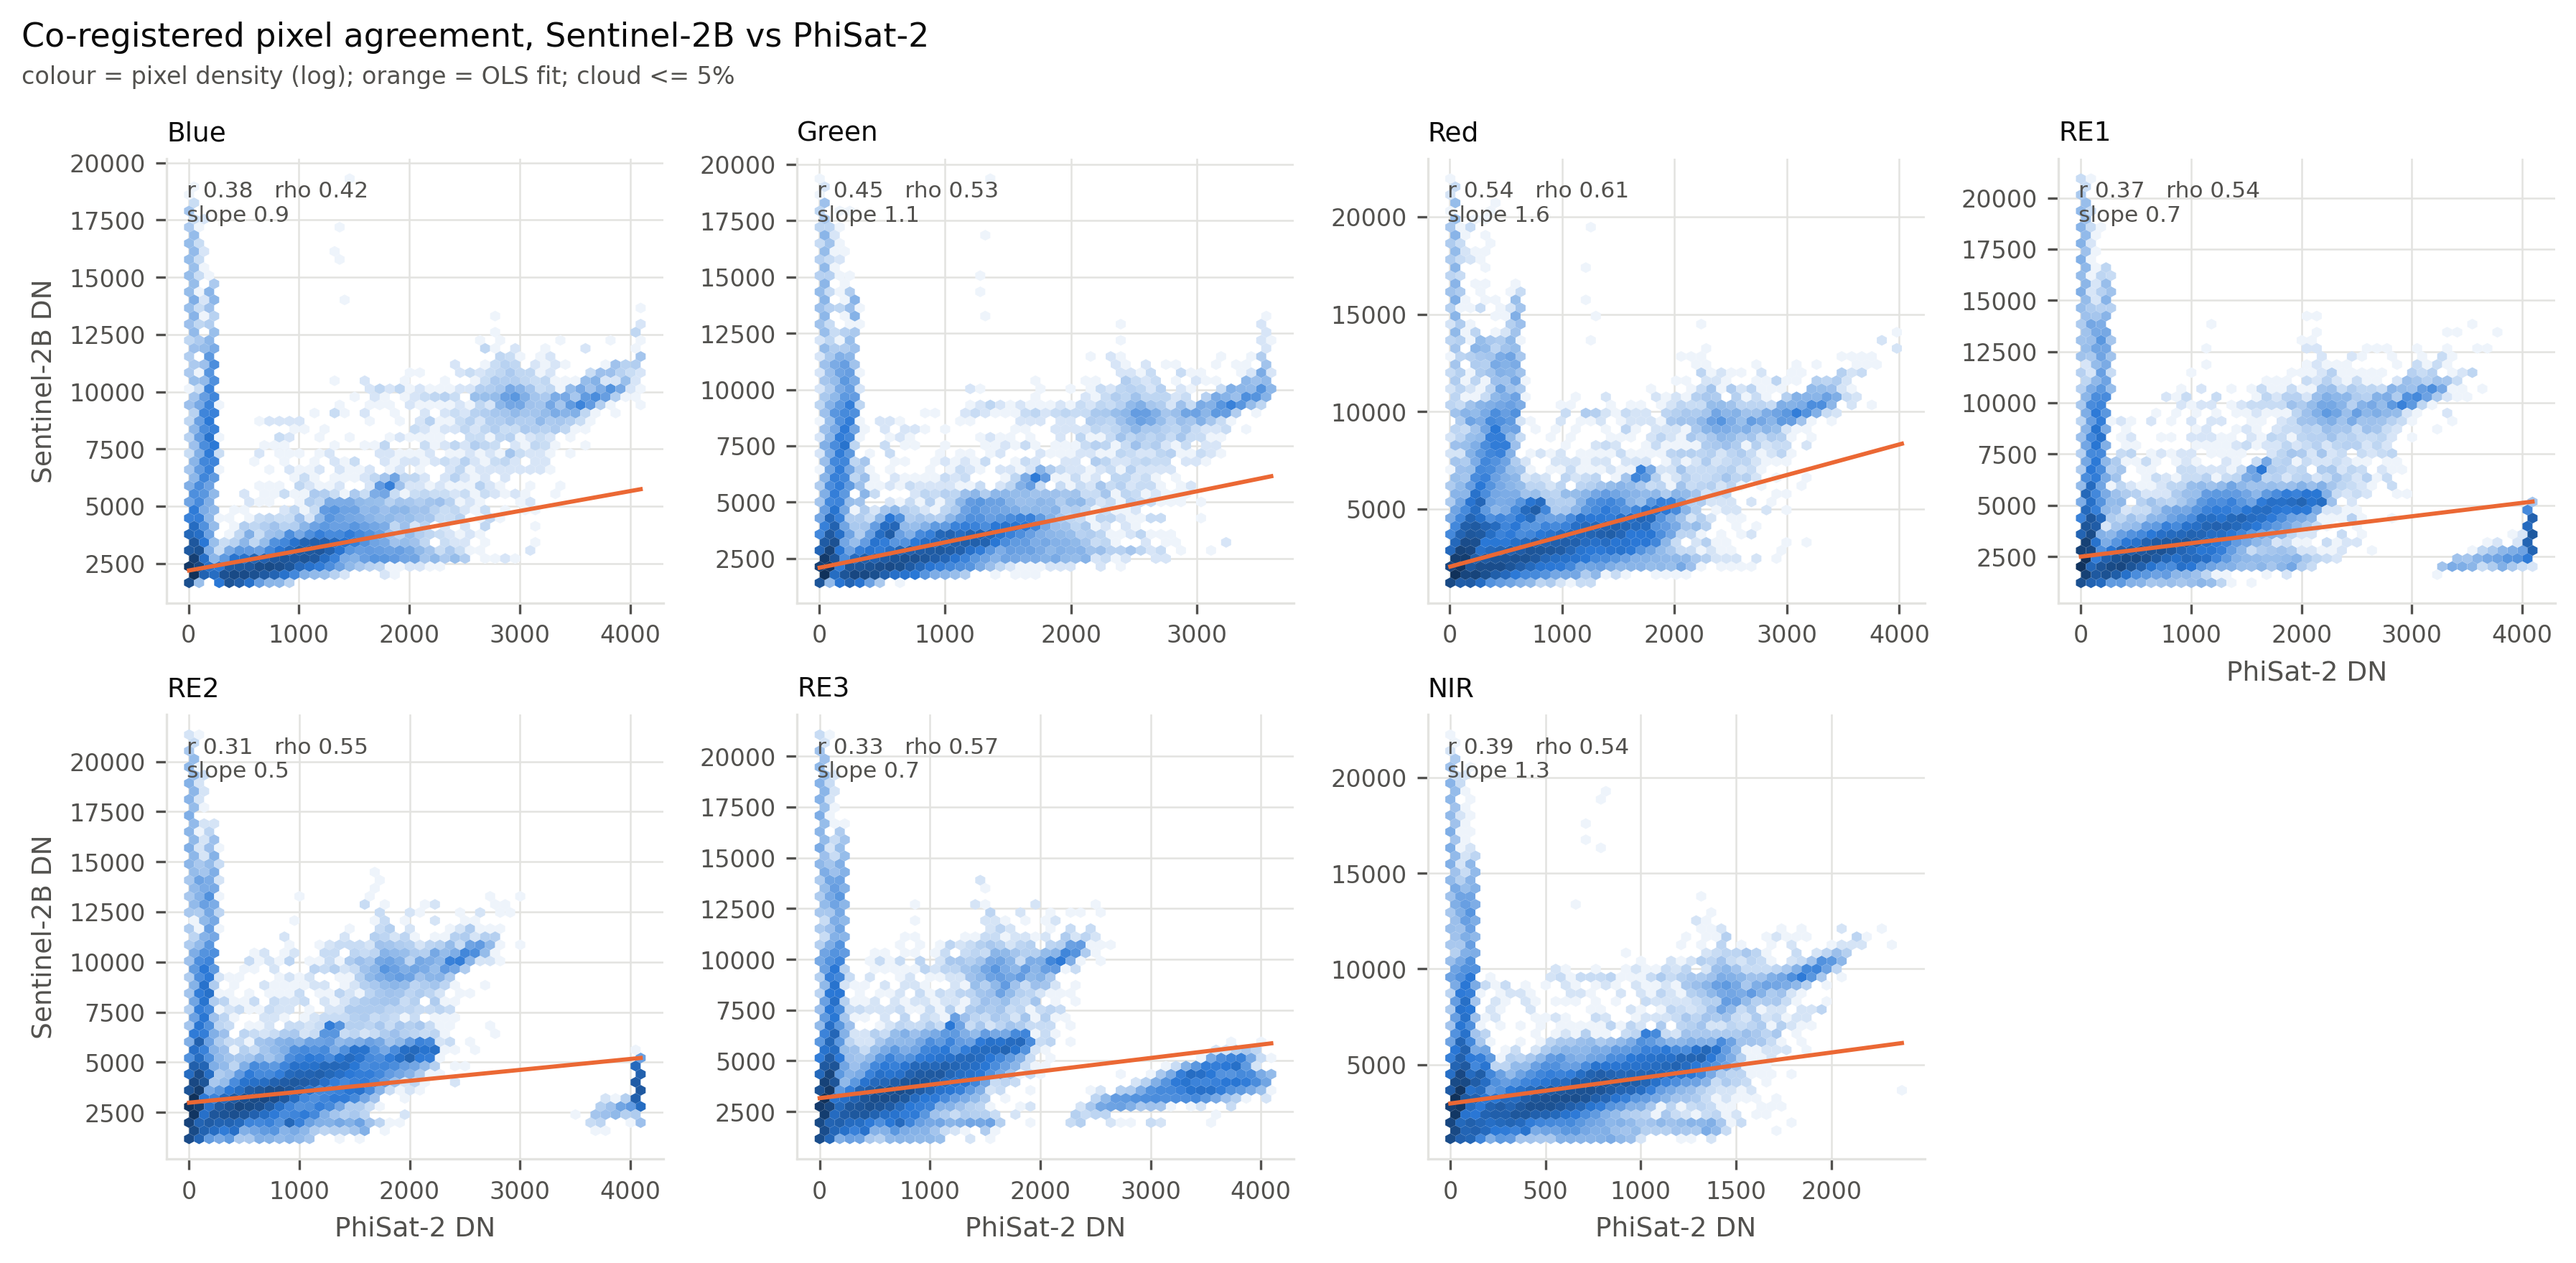
\includegraphics[width=\textwidth]{fig_sensor_scatter.png}
    \caption{Per-band pixel agreement between co-registered real-$\Phi$-sat-2 and Sentinel-2B digital numbers (hexbin density, log scale; orange = ordinary least-squares fit; patches with $\leq$5\% cloud only).
        Point clouds are diffuse around the fitted line in every band, and several bands (RE1, RE2) show a distinct vertical streak near zero $\Phi$-sat-2 DN spanning the full Sentinel-2 DN range, consistent with localized real-sensor dropout or saturation artifacts rather than measurement noise alone.
    }
    \label{fig:sensor-scatter}
\end{figure}

Third, and most directly relevant to the degradation-driver hypothesis discussed in Chapter~\ref{chap:results-discussion}, the shape of the spectral signature (each sensor's per-band median normalized by its own overall band mean, so that absolute scale is divided out) differs between real $\Phi$-sat-2 and Sentinel-2/simulated-$\Phi$-sat-2 (Figure~\ref{fig:spectral-signature}).
Sentinel-2 and the simulated domain are, again, visually indistinguishable from each other.
Real $\Phi$-sat-2, in contrast, shows a pronounced peak at the red band (1.85 relative to its own mean, against 0.85 for Sentinel-2/simulated) and a dip at the near-infrared band (0.70 against 1.21), a difference in relative spectral shape, not only absolute intensity.
This analysis is a quantitative support for attributing the domain gap primarily to spectral response function mismatch (Section~\ref{sec:rq1-results}) rather than to spatial resolution or noise level, since a resolution- or noise-driven gap would not be expected to alter the relative shape of the spectral signature this distinctly.

\begin{figure}[htp]
    \centering
    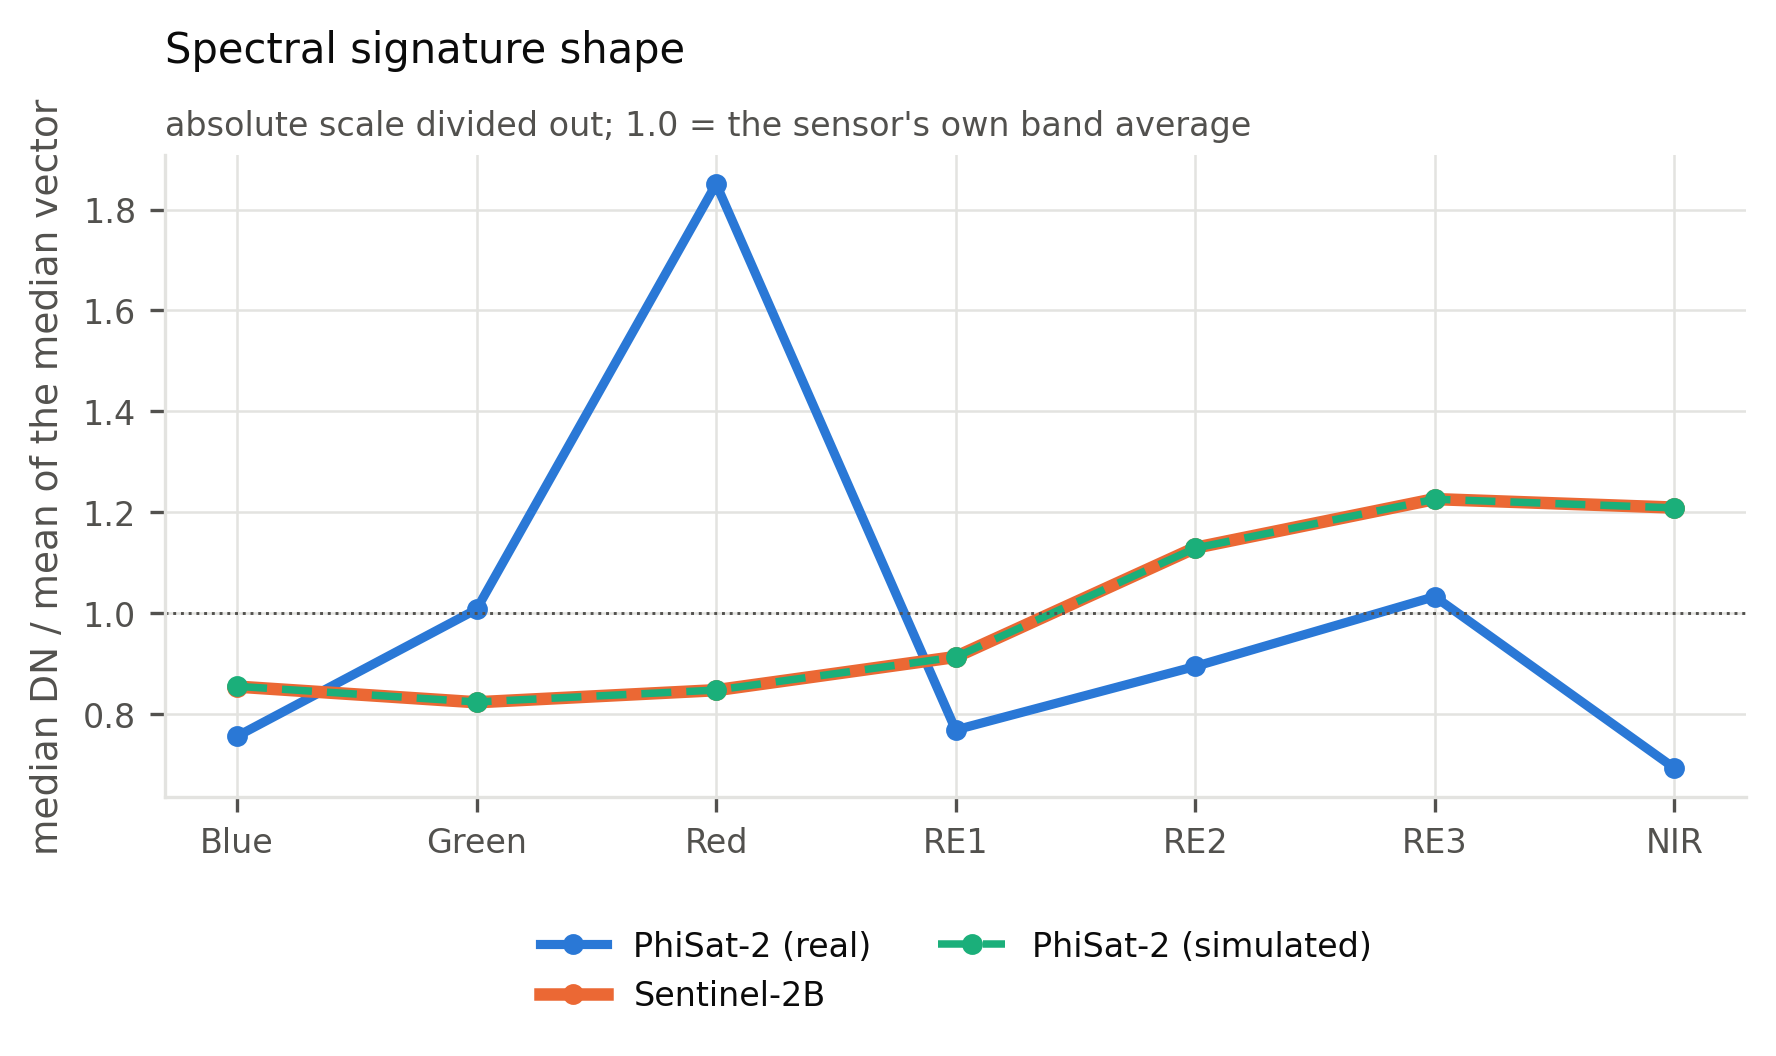
\includegraphics[width=0.7\textwidth]{fig_spectral_signature.png}
    \caption{Median per-band digital number, normalized by each sensor's own overall band mean (1.0 = that sensor's average).
        Sentinel-2B and simulated $\Phi$-sat-2 overlap almost exactly; real $\Phi$-sat-2 has a markedly different spectral shape, peaking at Red and dipping at RE1 and NIR.
    }
    \label{fig:spectral-signature}
\end{figure}

These measured per-domain statistics (mean, standard deviation, and clip value per band, computed separately for the real, Sentinel-2, and simulated domains) are what parametrize the per-domain normalization protocol of Section~\ref{sec:normalization}.

\subsection{Simulated degraded flood-segmentation dataset}
\label{sec:sen1floods-sim}

No real $\Phi$-sat-2 flood dataset exists, because the mission has not yet captured and labeled a flood event; this is a structural limitation of any new mission, not a data-collection oversight.
To obtain labeled data for the flood-segmentation task motivating this thesis, the Sen1Floods benchmark is passed through the same degradation pipeline used to build the triplets, producing a graded ladder of $\Phi$-sat-2-like flood scenes at increasing degradation severity.
This simulated dataset plays a different role from the triplets as it is the training and evaluation substrate for the flood task itself, not the substrate for measuring the domain gap, since it lacks a real-$\Phi$-sat-2 counterpart against which to validate the simulation directly.

The ladder is produced with an updated implementation of the OrbitalAI simulator, restructured as a configurable sequence of stages inside TerraTorch so that it applies to any Sentinel-2-based dataset in that framework rather than to a single acquisition.
The segmentation mask is carried through the transformation with the imagery (Section~\ref{sec:degradation-pipeline}, Figure~\ref{fig:simulator}).
This reimplementation allows to control each physical effect individually.
This gives the ladder a second purpose beyond supplying a simulated dataset with flood labels.
The triplets establish that a domain gap exists in TerraMind's representation (Section~\ref{sec:gap-measurement}) but not which physical difference between the two instruments produces it, and the two sensors differ in several respects at once, so no measurement on real pairs can separate the causes.
Degrading a fixed set of scenes one factor at a time, at graded severities within each factor makes that separation possible. The scene content is identical across the ladder by construction, so any change in the base TerraMind encoder's response is attributable to the effect being varied rather than to what the imagery depicts.
Chapter~\ref{chap:results-discussion} reports how the teacher responds across this ladder; isolating which individual factor carries the effect is key to answering RQ1.

\section{Physics-Based Sensor Degradation Pipeline}
\label{sec:degradation-pipeline}

The degradation pipeline adapts the simulator developed for the ESA $\Phi$-lab OrbitalAI challenge \cite{longepe2024orbitalai}, which projects labeled Sentinel-2 L1C tiles into the $\Phi$-sat-2 sensor domain by modeling the physical differences between the two instruments as a sequence of operations in radiance space.
Because these effects are defined physically on radiance, not reflectance, the pipeline converts source reflectance to top-of-atmosphere radiance, applies each degradation in turn, and converts back to reflectance to output a simulated L1C product.
Pixel coordinates are written $(i,j)$ and spectral band index $b_n$ throughout.

The implementation used here is an updated version of that simulator, summarised in Figure~\ref{fig:simulator}.
Each stage draws its parameters from its own intermediate input rather than from a single fixed configuration, so an individual effect can be varied or disabled without disturbing the others, which is what permits the factor-isolation use described in Section~\ref{sec:sen1floods-sim}.
Solar geometry and irradiance are retrieved per scene from the Copernicus Data Space OData API using the source product's location and acquisition time, so the radiance conversion of Equation~\eqref{eq:rad2refl} uses the true illumination conditions of each tile rather than a nominal value.

\begin{figure}[htp]
    \centering
    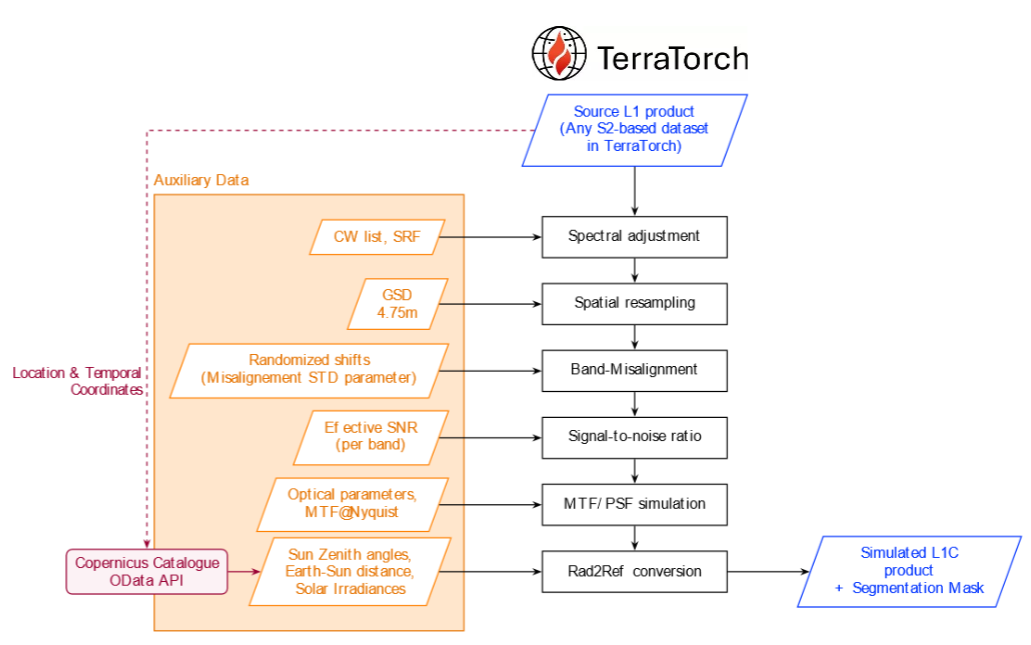
\includegraphics[width=\textwidth]{fig_updated_simulator.png}
    \caption{The updated degradation pipeline.
        A source Sentinel-2 L1 product passes through five physical stages in radiance space before conversion back to reflectance, each driven by its own auxiliary input: the centre-wavelength list and spectral response functions for the spectral adjustment, the 4.75\,m target ground sampling distance for the resampling, a misalignment standard deviation for the band-to-band shift, the per-band effective SNR for the noise term, and the Nyquist MTF for the optical blur.
        Solar zenith angle, Earth--Sun distance, and solar irradiance are retrieved per scene from the Copernicus Data Space OData API.
        Because every stage is parameterised separately, individual effects can be varied or switched off independently, and the segmentation mask is carried through the pipeline so that labels stay aligned with the degraded imagery.
    }
    \label{fig:simulator}
\end{figure}

\paragraph{Radiance--reflectance conversion.} TOA reflectance $\rho$ and TOA radiance $L$ are related by
\begin{equation}
    \rho(i,j,b_n) = \frac{\pi\, d^2}{E_{\text{SUN}}(b_n)\,\cos\theta_S(i,j)}\, L(i,j,b_n),
    \label{eq:rad2refl}
\end{equation}
where $d$ is the Earth--Sun distance in astronomical units, $E_{\text{SUN}}(b_n)$ the exo-atmospheric solar irradiance for band $b_n$, and $\theta_S(i,j)$ the solar zenith angle at pixel $(i,j)$.
The pipeline enters via the inverse of Equation~\eqref{eq:rad2refl} and exits by re-applying it after all radiance-domain degradations; solar irradiance and zenith angle are read from Sentinel-2 tile metadata via the Copernicus Data Space Ecosystem OData API, and no additional solar-irradiance adjustment is needed because Sentinel-2 and $\Phi$-sat-2 spectral bands are close enough in wavelength.
Earth--Sun distance is computed from acquisition day-of-year as $d = 1 - 0.01672\cos(0.9856(day - 4)\cdot \pi/180)$.

\paragraph{Spatial resampling.} $\Phi$-sat-2 has a uniform ground sampling distance of 4.75\,m across all bands; Sentinel-2 provides 10\,m (bands B2, B3, B4, B8) and 20\,m (bands B5, B6, B7).
Each band is resampled to the common 4.75\,m grid using bicubic interpolation, which limits the resampling artifacts that bilinear interpolation would introduce, though it cannot recover spatial detail the coarser source bands never captured.

\paragraph{Band-to-band misalignment.}
Push-broom acquisition co-registers spectral bands imperfectly, since detector rows are exposed at slightly different times and platform micro-vibration perturbs the line of sight during each band's integration window.
For the raw L1A product, the displacement of band $b_n$ relative to the previously acquired band follows
\begin{equation}
    \|\Delta \mathbf{r}(b_n)\| \sim \mathcal{N}(\mu_{b_n}, \sigma^2), \qquad \mu_{b_n} \in [0.44, 1.1]\ \text{pixels},
    \label{eq:misalign-l1a}
\end{equation}
with direction sampled uniformly over $[0, 2\pi)$ and displacement accumulating across preceding bands.
For the geometrically corrected L1C product used throughout this thesis, an on-board co-registration step removes this accumulation, and the residual is instead modeled as a single random displacement of each band relative to a reference band ($\mu_{b_n} = 0$), with standard deviation set higher over water ($\sigma_{\text{sea}} = 6$ pixels) than over land ($\sigma_{\text{land}} = 1$ pixel), reflecting the harder auto-registration problem posed by feature-poor sea surfaces.

\paragraph{Signal-to-noise degradation.} The baseline formulation draws a per-band noise sample from $\mathcal{N}(0,1)$ scaled by the ratio of a reference radiance to a specified SNR,
\begin{equation}
    L_{\text{noise}}(i,j,b_n) = \frac{L_{\text{ref}}(b_n)}{\text{SNR}(b_n)}\,\mathcal{N}(0,1), \label{eq:snr-const} \end{equation} which implicitly treats noise variance as signal-independent, matching the specified SNR only near $L_{\text{ref}}$.
A signal-dependent variant, consistent with a shot-noise regime in which SNR scales with the square root of collected signal, rescales the reference SNR to an effective, radiance-dependent value and samples
\begin{equation}
    L_{\text{noise}}(i,j,b_n) = \frac{\sqrt{L_{\text{in}}(i,j,b_n)\,L_{\text{ref}}(b_n)}}{\text{SNR}(b_n)}\,\mathcal{N}(0,1).
    \label{eq:snr-signal}
\end{equation}
The implementation used for the calibrated baseline degradation level applies Equation~\eqref{eq:snr-signal}.
The extended sweep pushes beyond nominal $\Phi$-sat-2 noise conditions, since domain-invariance has to be stress-tested under more severe degradation than the flight-validated parameters cover.
For that sweep, a simplified variant samples a base SNR uniformly from a specified range and scales noise by the ratio of that SNR to the batch-wise maximum radiance, trading exact photometric fidelity for the ability to sweep degradation severity beyond the calibrated regime.
This trade-off is stated explicitly here because it is a deliberate design choice, not an approximation error: the baseline level is flight-parameter-calibrated, and only the extended sweep sacrifices fidelity for range.

\paragraph{Optical blur via MTF/PSF.}
Optical blur is modeled through the system modulation transfer function (MTF), aggregating static (optics, detector), dynamic (jitter, platform instability), and smearing (motion) contributions.
Assuming shift-invariant blur, imaging reduces to convolution with the system point spread function (PSF).
Given the MTF amplitude at Nyquist frequency $M(b_n)$, the MTF is modeled as Gaussian in normalized spatial frequency $k$,
\begin{equation}
    \text{MTF}(b_n, k) = e^{\ln M(b_n) \cdot k^2},
    \label{eq:mtf}
\end{equation}
with the corresponding PSF obtained as its inverse Fourier transform and convolved with the radiance image.
For $\Phi$-sat-2 the average Nyquist MTF is $M_\Phi(b_n) \approx 0.05$; for Sentinel-2, $M_{\text{S-2}}(b_n) \approx 0.30$.
The reference simulation applies Equation~\eqref{eq:mtf} directly with $M_\Phi(b_n)$, leaving the intrinsic Sentinel-2 blur uncorrected; a combined-filter form exists for the case where source blur should also be compensated, but is not required here since the intrinsic Sentinel-2 blur is small relative to $\Phi$-sat-2's.

This pipeline is shared infrastructure within the research group: it also underlies the pre-training and benchmark datasets used by $\Phi$satNet (Section~\ref{sec:phisatnet-background}).
This thesis uses the pipeline's output in a new way, by stress-testing the base TerraMind encoder across a ladder of degradation severities to isolate which physical effect drives the domain gap, and by using it to produce a simulated flood-segmentation dataset in the absence of any real $\Phi$-sat-2 flood data.

\section{Domain Gap Measurement}
\label{sec:gap-measurement}

\subsection{Normalization protocol}
\label{sec:normalization}

Raw $\Phi$-sat-2 digital numbers are heavy-tailed; a square-root transform is applied first to bring the distribution closer to Gaussian, followed by a smooth (soft-saturating) clip toward a domain-specific clip value rather than a hard clip, and finally per-domain $z$-score standardization using mean and standard deviation statistics computed separately for each sensor domain (real $\Phi$-sat-2, real Sentinel-2, simulated $\Phi$-sat-2), rather than a single shared normalization applied across domains.
An early baseline was corrupted by a normalization defect that caused weight saturation and an artificially depressed performance estimate; correcting it was a precondition for every result reported in Chapter~\ref{chap:results-discussion}.

Because per-domain normalization could itself account for an apparent domain gap that is really just a difference in raw value scale, the domain-gap measurement below was run both with and without per-domain normalization.
The two conditions produced similar overall results, and per-domain normalization produced lower cosine similarity between domains in the encoder's early layers, the opposite of what a normalization artifact would predict, indicating that the measured gap in early layers is a genuine representational effect rather than a calibration artifact.

\subsection{Direct and indirect evidence}

The domain gap is measured directly, in latent space, using the co-registered triplets: paired cosine similarity between the embeddings of the two sensor views of the same ground, proxy $\mathcal{A}$-distance (PAD) computed per encoder layer to locate where the gap concentrates, and a cross-domain linear-probe-transfer test in which a probe fitted on one sensor's embeddings is applied to the other's embeddings of the same patches.
It is measured indirectly through downstream task performance: LULC mIoU of the distilled student relative to a supervised baseline of identical architecture trained directly on the target sensor (Section~\ref{sec:evaluation-protocol}), and flood-segmentation IoU across the simulated degradation ladder of Section~\ref{sec:sen1floods-sim}.

\section{Domain-Adaptation Strategy}
\label{sec:da-mechanism}

\subsection{Fine-tuning on degraded data}
\label{sec:da-negative-result}

The first mechanism attempted was implicit: fine-tune TerraMind's encoder on the LULC task using degraded, simulated training data, on the premise that exposure to degraded examples during training would itself induce a more domain-invariant representation.
Cross-validation against the real-$\Phi$-sat-2/Sentinel-2 triplets showed that it doesn't hold. A model fine-tuned this way doesn't show lower domain gap to real $\Phi$-sat-2 than a model fine-tuned only on clean Sentinel-2.
Standard supervised fine-tuning, even on physics-degraded data produced by a physics-based simulator, doesn't translate into a sensor-invariant representation.

\subsection{Domain-specific batch normalization}
\label{sec:dsbn-mechanism}

The mechanism adopted only requires that the domain of each training example is known.
Domain-Specific Batch Normalization (DSBN) \cite{chang2019dsbn} gives the student a separate batch-normalization affine transform and running statistics per sensor domain, on top of otherwise fully shared convolutional weights.
Concretely, the two-branch distillation scheme (Section~\ref{sec:kd}) forwards a Sentinel-2 batch and a $\Phi$-sat-2 batch through the student separately in each training step; DSBN lets each pass use its own domain's normalization statistics rather than a single statistics set blended across both.
Figure~\ref{fig:dsbn} contrasts the two arrangements.
Under ordinary batch normalization both domains pass through one shared layer, so its running statistics converge to a blend of the two sensors and describe neither exactly.
A DSBN layer instead holds two branches, and each example activates the branch matching its own domain while the inactive branch is left untouched.
Everything outside those layers, which is to say every convolutional weight in the student, stays shared and is therefore trained on both sensors at once, so the mechanism separates the sensor-specific part of the representation (per-channel scale and shift) from the part that ought to be common (the learned filters).

\begin{figure}[htp]
    \centering
    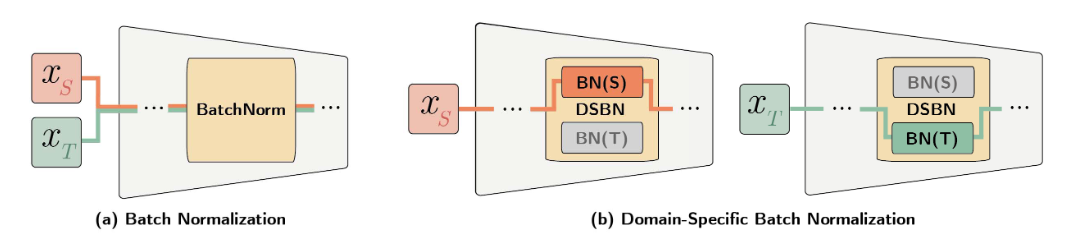
\includegraphics[width=\textwidth]{fig_bn_dsbn.png}
    \caption{Batch normalization compared with domain-specific batch normalization, from Chang et al.~\cite{chang2019dsbn}.
        (a) A single BatchNorm layer processes source ($x_S$) and target ($x_T$) examples alike, so its statistics describe a mixture of the two domains.
        (b) A DSBN layer carries one branch per domain, and each input is routed to the branch corresponding to its own domain; the other branch, shown greyed, is inactive for that example.
        All parameters outside the DSBN layers remain shared across domains.
        In this thesis the source domain is Sentinel-2 and the target domain is $\Phi$-sat-2, and the domain of every input is known both during training and on board.
    }
    \label{fig:dsbn}
\end{figure}
Because the deployed sensor on board $\Phi$-sat-2 is always known at inference, selecting the matching normalization branch at deployment time costs nothing operationally, unlike a sensor-agnostic representation, which would need to be invariant without ever being told which sensor produced a given input.

Since the student must eventually run on the target hardware (Myriad~2), we have to measure the cost of the DSBN mechanism and its implication on the model architecture.
Batch normalization is representable in the deployment format: \texttt{BatchNormInference} belongs to \texttt{opset1}, the earliest OpenVINO operator set, and is therefore within the operator set available to the 2020.3 release that supports this processor.
\footnote{\url{https://docs.openvino.ai/2023.3/openvino_docs_ops_normalization_BatchNormInference_1.html}.
    Operator specifications are versioned by opset rather than by release; the 2020.3 documentation set has been withdrawn by Intel, so the current page is cited for an operator whose opset membership predates it.
}
In practice, however, the operator is not emitted at all, because at inference a batch-normalization layer reduces to a fixed per-channel affine transform.
OpenVINO's model conversion folds the transform into the weights of the preceding convolution by default.
Domain-specific normalization changes only how many such constant sets exist during training, with one per sensor domain.
Because the acquiring instrument is always known on board, only the target-sensor branch is exported, and its statistics fold into the convolution weights as a single-domain model's would.
The deployed graph therefore carries no batch-normalization operation, and DSBN adds neither operator-support risk nor inference cost relative to the supervised baseline: its additional parameters exist only while training.
This argument follows from the documented conversion behaviour of the toolchain rather than from a completed export of the student to the $\Phi$-sat-2 processor, which has not been carried out.

\subsection{Paired-contrastive triplet alignment}
\label{sec:contrastive-mechanism}

The co-registered triplet dataset provides something most domain-adaptation settings lack: for every training example, the identical underlying scene observed by two or three different sensors.
This guarantees a directly supervised alignment objective rather than an unpaired one.
The contrastive loss pulls the embeddings of matched real-$\Phi$-sat-2, real-Sentinel-2, and simulated-$\Phi$-sat-2 patches of the same scene together, while pushing apart embeddings of unrelated scenes, regardless of which sensor produced each embedding.
This directly penalizes the encoder for representing sensor identity, rather than only scene content, and does so using the strongest available supervisory signal, exact scene correspondence, instead of matching marginal distributions between unpaired sensor domains as an MMD-style objective would.

This objective was implemented and evaluated on top of the DSBN configuration above, with the co-registered triplets used as designed: to test a training mechanism, not only to measure the gap.
On the LULC task, it did not improve downstream performance beyond the DSBN-only configuration (Section~\ref{sec:rq2-results}), and all headline results in Chapter~\ref{chap:results-discussion} are reported with its weight set to zero.
This is reported as a negative ablation result rather than omitted: the co-registered pairing that makes a contrastive objective possible is a genuine structural asset of this dataset, and the fact that exploiting it directly added nothing measurable on top of a much simpler per-domain normalization scheme is itself informative about where the sensor gap actually lives (Section~\ref{sec:rq1-results}) and about how much machinery is actually needed to close it.

\section{Cross-Architecture Knowledge Distillation}
\label{sec:kd}

TerraMind's ViT-based encoder cannot run on the $\Phi$-sat-2 on-board processor: the Myriad 2 VPU's supported operator set has no dynamic-axes support, which ViT inference requires regardless of model size.
Therefore, compression must cross architecture families, from ViT teacher to CNN student, rather than compress within the ViT family as some prior on-board GeoFM work does\cite{du2025onorbitdemonstrationgeospatialfoundation}.
The teacher is TerraMind in its base variant, fine-tuned on the Sentinel-2 branch of the triplet dataset for the LULC task and then frozen.
The student is a U-Net\cite{ronneberger2015unet} trained from random initialisation. It was chosen for its simple encoder-decoder structure, which is a natural fit for the segmentation task, and for its low operator set requirements, which are compatible with the Myriad 2 VPU as demonstrated by the $\Phi$satNet baseline (Section~\ref{sec:phisatnet-background}).

Two placements for a domain-adaptation mechanism were considered: baking invariance into the frozen teacher and letting the student inherit it passively by mimicking the teacher's outputs, or giving the student its own adaptation mechanism directly.
This thesis adopts the second, for a reason independent of which specific mechanism is used. The student model, is to be deployed, so whatever mechanism is used should be evaluated on the student's own representation rather than assumed to transfer from the teacher.
Two candidate mechanisms were implemented at the student level: domain-specific batch normalization (Section~\ref{sec:dsbn-mechanism}), adopted as the mechanism responsible for every headline result in Chapter~\ref{chap:results-discussion}, and a paired-contrastive triplet loss (Section~\ref{sec:contrastive-mechanism}), evaluated as an ablation on top of it and found not to improve downstream performance further.
DSBN also incidentally repairs a train/test inconsistency inherent to the two-branch training scheme: the two sensors are forwarded in separate passes, so during training each pass would otherwise be normalized by its own domain's batch statistics while a single shared set of running averages (a blend of both domains) is used at inference, meaning the encoder would never encounter, at test time, the normalization under which it was optimised.
Giving each domain its own running statistics closes this gap as a side effect of the same mechanism.

Figure~\ref{fig:kd-architecture} sets out the resulting training scheme.
Its defining feature is that the teacher is queried only on Sentinel-2, the domain it was pre-trained and fine-tuned on and the only one on which its predictions are trustworthy.
A single teacher forward pass then supervises both student branches, so the student's $\Phi$-sat-2 predictions are distilled against a teacher output computed from the Sentinel-2 view of the same ground.
This transfer of supervision across sensors is possible only because the two views are co-registered, and it keeps the teacher's own domain-shift error out of the student. Querying the teacher directly on $\Phi$-sat-2 would distil that error rather than correct it.

\begin{figure}[htbp]
    \centering
    \resizebox{\textwidth}{!}{%
        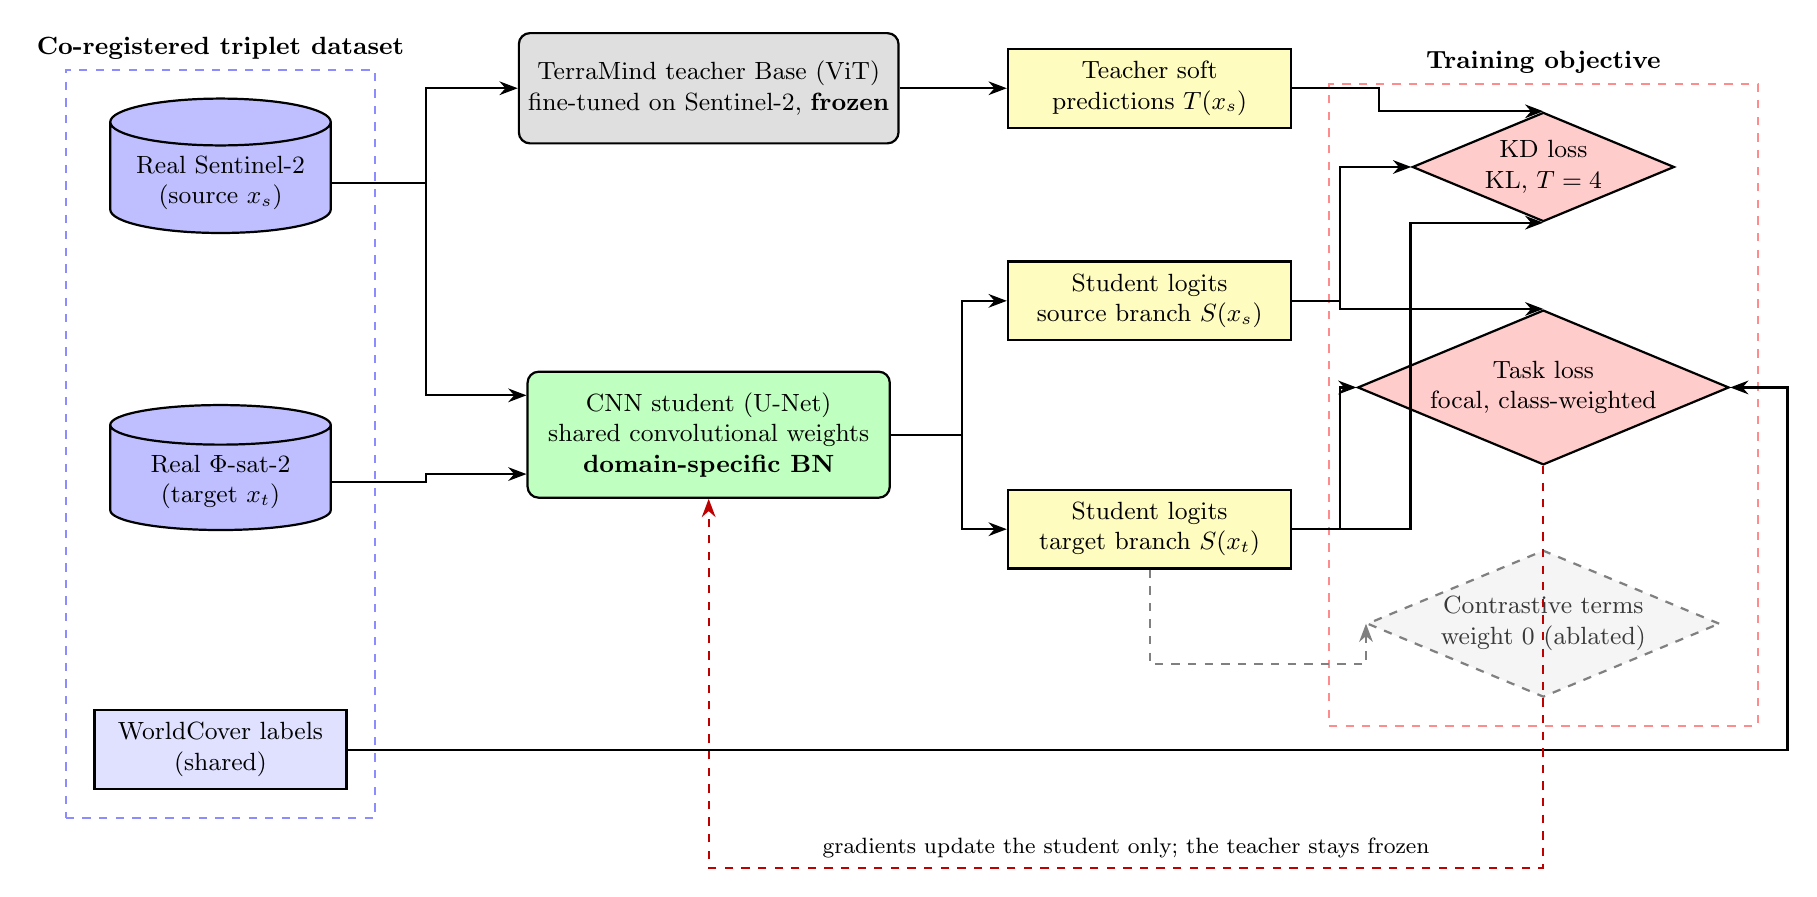
\begin{tikzpicture}[
                >=Stealth,
                font=\small,
                database/.style={cylinder, draw, shape border rotate=90, aspect=0.25, align=center,
                        fill=blue!25, minimum height=1.2cm, minimum width=2.8cm, thick},
                frozen/.style={rectangle, draw, rounded corners, align=center, fill=gray!25,
                        minimum width=4.6cm, minimum height=1.4cm, thick},
                model/.style={rectangle, draw, rounded corners, align=center, fill=green!25,
                        minimum width=4.6cm, minimum height=1.6cm, thick},
                feature/.style={rectangle, draw, align=center, fill=yellow!25,
                        minimum width=3.6cm, minimum height=1.0cm, thick},
                labels/.style={rectangle, draw, align=center, fill=blue!12,
                        minimum width=3.2cm, minimum height=1.0cm, thick},
                loss/.style={diamond, draw, align=center, fill=red!20, aspect=2.4, thick,
                        minimum width=2.8cm, inner sep=1pt},
                ablated/.style={diamond, draw=gray, dashed, align=center, fill=black!4,
                        text=gray!45!black, aspect=2.4, thick, minimum width=2.8cm, inner sep=1pt},
                arrow/.style={->, thick},
                backarrow/.style={->, thick, red!75!black, dashed},
            ]

            % --- data -------------------------------------------------------
            \node[database] (data_s2)  at (0,  2.8) {Real Sentinel-2\\(source $x_s$)};
            \node[database] (data_phi) at (0, -1.0) {Real $\Phi$-sat-2\\(target $x_t$)};
            \node[labels]   (mask)     at (0, -4.4) {WorldCover labels\\(shared)};

            % --- models -----------------------------------------------------
            \node[frozen] (teacher) at (6.2,  4.0)
            {TerraMind teacher Base (ViT)\\fine-tuned on Sentinel-2, \textbf{frozen}};
            \node[model]  (student) at (6.2, -0.4)
            {CNN student (U-Net)\\shared convolutional weights\\\textbf{domain-specific BN}};

            % --- outputs ----------------------------------------------------
            \node[feature] (t_soft)   at (11.8,  4.0) {Teacher soft\\predictions $T(x_s)$};
            \node[feature] (s_source) at (11.8,  1.3) {Student logits\\source branch $S(x_s)$};
            \node[feature] (s_target) at (11.8, -1.6) {Student logits\\target branch $S(x_t)$};

            % --- losses -----------------------------------------------------
            \node[loss]    (kd)   at (16.8,  3.0) {KD loss\\KL, $T=4$};
            \node[loss]    (task) at (16.8,  0.2) {Task loss\\focal, class-weighted};
            \node[ablated] (con)  at (16.8, -2.8) {Contrastive terms\\weight $0$ (ablated)};

            % --- forward routing --------------------------------------------
            \draw[arrow] (data_s2.east)  -- ++(1.2,0) |- (teacher.west);
            \draw[arrow] (data_s2.east)  -- ++(1.2,0) |- ([yshift=5mm]student.west);
            \draw[arrow] (data_phi.east) -- ++(1.2,0) |- ([yshift=-5mm]student.west);

            \draw[arrow] (teacher.east) -- (t_soft.west);
            \draw[arrow] (student.east) -- ++(0.9,0) |- (s_source.west);
            \draw[arrow] (student.east) -- ++(0.9,0) |- (s_target.west);

            % one teacher output supervises BOTH student branches
            \draw[arrow] (t_soft.east)   -- ++(1.1,0) |- (kd.north);
            \draw[arrow] (s_source.east) -- ++(0.6,0) |- (kd.west);
            \draw[arrow] (s_target.east) -- ++(1.5,0) |- (kd.south);

            \draw[arrow] (s_source.east) -- ++(0.6,0) |- (task.north);
            \draw[arrow] (s_target.east) -- ++(0.6,0) |- (task.west);
            \draw[arrow] (mask.east) -- (19.9,-4.4) -- (19.9,0.2) -- (task.east);

            \draw[arrow, gray, dashed] (s_target.south) -- ++(0,-1.2) -| (con.west);

            % --- backpropagation --------------------------------------------
            \draw[backarrow] (task.south) -- (16.8,-5.9) -- node[above, black]
            {\footnotesize gradients update the student only; the teacher stays frozen}
            (6.2,-5.9) -- (student.south);

            % --- grouping ---------------------------------------------------
            \begin{scope}[on background layer]
                \node[draw, dashed, thick, blue!45, inner sep=0.35cm, fit=(data_s2) (data_phi) (mask),
                    label=above:\textbf{Co-registered triplet dataset}] {};
                \node[draw, dashed, thick, red!45, inner sep=0.35cm, fit=(kd) (task) (con),
                    label=above:\textbf{Training objective}] {};
            \end{scope}
        \end{tikzpicture}%
    }
    \caption{Cross-architecture distillation with domain-specific normalization.
        The frozen TerraMind teacher is evaluated only on the Sentinel-2 view, where it is trustworthy; its soft predictions supervise both student branches, which is possible because the two sensor views depict the same scene.
        The student is forwarded twice per patch, once per sensor, selecting its own batch-normalization statistics each time while sharing all convolutional weights.
        Both branches also receive the task loss against the single shared WorldCover label map.
        The contrastive terms were implemented and evaluated but carry zero weight in every result reported in Chapter~\ref{chap:results-discussion}.
    }
    \label{fig:kd-architecture}
\end{figure}

The distilled student is therefore domain-adaptive rather than domain-invariant in the strict sense: convolutional weights are shared across sensors, but normalization statistics are not, and the correct branch must be selected at inference according to which sensor produced the input.
This is a weaker property than a single sensor-agnostic representation, but it is the property an on-board deployment actually needs, since the acquiring instrument is always known at inference time.
This is unlike a model expected to generalize to sensors it never saw during training.

\section{Evaluation Protocol}
\label{sec:evaluation-protocol}

Four evaluations follow from the mechanisms above, corresponding to the three research questions of Section~\ref{sec:research-objective}.
First (RQ1), whether the sensor gap is visible in the teacher's representation itself: paired cosine similarity, per-layer PAD, and cross-domain linear-probe transfer between the two sensor views of the same co-registered patches.
Second (RQ2), whether the distilled student's representation inverts these measurements relative to the teacher, and which of the two candidate mechanisms (DSBN, contrastive alignment) is responsible.
Third (RQ3), whether distillation with the adopted mechanism improves LULC task performance over a supervised baseline of identical student architecture trained directly on labelled $\Phi$-sat-2 with no teacher and no second sensor, at a label budget large enough to be representative and, separately, at a much smaller budget, since the direction of this comparison is not assumed to be constant across label budgets.
Fourth, flood segmentation across the simulated degradation ladder, to characterize how gracefully performance degrades with increasing sensor-noise severity.
A few-shot label-efficiency comparison against $\Phi$satNet (Section~\ref{sec:phisatnet-background}) on matched small label budgets, testing directly whether adapting TerraMind's broad, diverse pre-training generalizes to $\Phi$-sat-2 with fewer labels than $\Phi$satNet's mission-specific pre-training requires, remains planned but has not been run (Section~\ref{sec:discussion-comparison}).
The earlier protocol of fully fine-tuning TerraMind directly on real $\Phi$-sat-2 LULC labels, evaluated on the same real domain without any cross-sensor test, produced a baseline mIoU that is retained in Appendix~\ref{app:real-baseline} for reference, but it is not the main baseline of interest because it does not test cross-sensor generalization and therefore does not address the research questions of this thesis.

\section{Tools, Software Environment, and Reproducibility}
\label{sec:reproducibility}

The degradation pipeline and dataset construction are implemented as modular EOTask objects within the \texttt{eo-learn} framework, orchestrated through a versioned simulation configuration object rather than hard-coded parameters, so that a given degradation run (baseline-calibrated or extended-sweep) is fully specified by its configuration rather than by code edits.
Triplet and LULC datasets are stored in HDF5 with an accompanying manifest recording per-patch provenance and train/validation/test split assignment (fixed random seed, positional split), enabling exact reproduction of any reported split.
Model training (TerraMind fine-tuning, DSBN-based distillation, the contrastive-alignment ablation) is implemented in PyTorch.
The codebase is organized as a single versioned Python package with submodules separating data simulation, dataset loading, model training tasks, and drift analysis, under standard git version control, so that each experiment reported in Chapter~\ref{chap:results-discussion} corresponds to a specific, retrievable commit and configuration.

\chapter{Results and Discussion}
\label{chap:results-discussion}

This chapter reports the experiments that evaluate the three research questions of Section~\ref{sec:research-objective}: whether a measurable sensor domain gap exists in the latent space of a geospatial foundation model, where it concentrates and which physical sensor difference produces it (RQ1), whether cross-architecture distillation from that model can produce a sensor-adaptive compact student (RQ2), and whether doing so is preferable to simply training the compact model on the target sensor directly (RQ3).
All the results below use the single configuration set out in Section~\ref{sec:configuration}, which is a distillation with domain-specific batch normalization, and the comparison of interest throughout is against a supervised baseline of identical architecture trained without any distillation.
With one exception, every condition reported in this chapter was run once, with a single fixed seed.
We therefore report the comparisons descriptively, as differences between training curves and between best-epoch scores, and not as statistical inferences.
The epoch-to-epoch validation variance is of the order of $0.02$ mIoU, so differences smaller than roughly $0.03$ should not be treated as resolved.
The exception is the degradation-ladder evaluation of Section~\ref{sec:ladder-results}, which we replicated over three seeds and for which the drops are reported with a measured seed-to-seed deviation.
That section is consequently the only one in this chapter whose smaller effects are resolved.

\section{Experimental Configuration}
\label{sec:configuration}

The teacher is TerraMind~\cite{jakubik2025terramind} at the \texttt{base} scale, fine-tuned on the Sentinel-2 branch of the triplet dataset (Section~\ref{sec:triplets}) for the eleven-class WorldCover LULC task~\cite{zanaga2022worldcover}, and frozen thereafter.
The student is a U-Net~\cite{ronneberger2015unet} with $9.85$\,M parameters, trained from a random initialisation, since no pre-trained weights are available for this backbone.
This is a material constraint, and we return to it in Section~\ref{sec:limitations}.
Both models consume the seven-band Blue--NIR stack under the per-domain normalization protocol of Section~\ref{sec:normalization}.

Two elements of this configuration deserve to be stated explicitly, since we arrived at both of them empirically and both of them materially change the results.

\paragraph{Domain-specific batch normalization.}
The student carries a separate set of batch-normalization~\cite{ioffe2015batchnorm} statistics and affine parameters for each sensor, with all convolutional weights shared, following Chang et al.~\cite{chang2019dsbn}.
Beyond its role as a domain-adaptation mechanism, this also corrects a train/test inconsistency that is inherent to the two-branch training scheme.
The two sensors are forwarded in separate passes, so during the training each pass is normalized by the batch statistics of its own domain, while a single shared set of running averages, which is a blend of the two domains, is what would be used at inference.
The encoder would therefore never encounter at test time the normalization under which it was optimised.

\paragraph{Class-imbalanced task loss.}
The WorldCover class prior on this dataset is severely imbalanced: the three rarest classes (snow/ice, mangroves, moss/lichen) together account for $1.2\%$ of labelled pixels but, under a macro-averaged mIoU, for $27\%$ of the metric.
Under unweighted cross-entropy the student never predicted these classes at all, scoring exactly zero IoU on them in training as well as validation, a failure to learn, not overfitting.
All the runs reported here therefore use a focal loss~\cite{lin2017focal} with $\gamma = 2$, and an inverse-square-root class weighting derived from the measured pixel frequencies, which is a milder variant of the effective-number scheme of Cui et al.~\cite{cui2019classbalanced}.

The contrastive representation-alignment objectives (Section~\ref{sec:contrastive-mechanism}) were implemented and ablated, but they are disabled in all the results below, since their weights are zero throughout.
That ablation is reported separately and it is not the subject of this chapter.

Table~\ref{tab:hyperparameters} lists the settings of both arms.
Everything the two conditions could share is held constant: architecture, initialisation, split, seed, normalization, augmentation, task loss, optimiser, schedule, and early-stopping criterion are identical, and the arms differ only in the presence of the teacher, the second sensor branch, and domain-specific normalization.

\begin{table}[htbp]
    \centering
    \label{tab:hyperparameters}
    \begin{tabular}{lll}
        \toprule
        Setting                 & KD + DSBN                                                                             & Supervised baseline \\
        \midrule
        \multicolumn{3}{l}{\emph{Shared}}                                                                                                     \\
        Student architecture    & \multicolumn{2}{l}{U-Net, 7 input bands, 32 decoder channels, $1{\times}1$ conv head}                       \\
        Initialisation          & \multicolumn{2}{l}{Random (no pre-trained weights available)}                                               \\
        Optimiser               & \multicolumn{2}{l}{AdamW}                                                                                   \\
        Learning rate           & \multicolumn{2}{l}{$1\times10^{-4}$}                                                                        \\
        Weight decay            & \multicolumn{2}{l}{$1\times10^{-4}$}                                                                        \\
        LR schedule             & \multicolumn{2}{l}{ReduceLROnPlateau, factor $0.5$, patience $5$}                                           \\
        Batch size              & \multicolumn{2}{l}{$8$ patches}                                                                             \\
        Early stopping          & \multicolumn{2}{l}{Patience $12$ on target-sensor validation IoU}                                           \\
        Model selection         & \multicolumn{2}{l}{Best target-sensor validation IoU}                                                       \\
        Task loss               & \multicolumn{2}{l}{Focal, $\gamma = 2.0$}                                                                   \\
        Class weighting         & \multicolumn{2}{l}{Inverse square-root of measured pixel frequency}                                         \\
        Augmentation            & \multicolumn{2}{l}{Joint geometric (flips, $90^{\circ}$ rotations)}                                         \\
        Random seed             & \multicolumn{2}{l}{$42$}                                                                                    \\
        Numerical precision     & \multicolumn{2}{l}{$32$-bit}                                                                                \\
        \midrule
        \multicolumn{3}{l}{\emph{Distillation-specific}}                                                                                      \\
        Teacher                 & TerraMind, frozen                                                                     & ---                 \\
        Distillation loss       & KL on logits, $T = 4.0$                                                               & ---                 \\
        Distillation applied to & All pixels, both branches                                                             & ---                 \\
        Task-loss weight        & $1.0$ target $+$ $1.0$ source                                                         & $1.0$ target        \\
        Distillation weight     & $1.0$                                                                                 & ---                 \\
        Contrastive weights     & $0$ (instance and pixel)                                                              & ---                 \\
        Domain-specific BN      & Enabled                                                                               & ---                 \\
        Sensor branches         & Two ($\Phi$-sat-2, Sentinel-2)                                                        & One ($\Phi$-sat-2)  \\
        \bottomrule
    \end{tabular}
    \caption{Training configuration for the two arms.
        Settings above the rule are identical by construction; those below apply to the distilled arm only.
    }
\end{table}

One asymmetry in this comparison is structural rather than incidental, and it should be stated alongside the table.
The distilled arm applies the task loss to both sensor views of each patch, so within one epoch it draws twice as much supervision from the same labels as the single-branch baseline does.
This is inherent to what the comparison is testing, since the baseline has no second view by definition, but it does mean that the per-epoch comparisons reported below are not matched on gradient signal, and it also contributes, alongside the forward pass of the frozen teacher, to the cost difference quantified in Section~\ref{sec:rq3-results}.

\wip{A second ablation, isolating domain-specific normalization from distillation itself, is in progress and is not reported here.
    It requires a distilled student trained with a single shared set of batch-normalization statistics, which is the condition that would separate the contribution of the domain-specific variant from that of the two-branch distillation scheme and the class-balanced loss adopted alongside it.
    Until that run completes, the attribution of the invariance results of Section~\ref{sec:rq2-results} to domain-specific normalization specifically should be read as provisional: what the results below establish is that the configuration as a whole produces the reported behaviour, not which of its components is responsible.
}

\section{Sensor Gap in TerraMind Latent Space (RQ1)}
\label{sec:rq1-results}

The first question is whether the domain gap is visible in the representation itself, and not only in the downstream accuracy.
We extracted embeddings for $800$ co-registered test patches from both sensors, and compared them under three measures: the paired cosine similarity between the two views of the same ground, the proxy $\mathcal{A}$-distance (PAD)~\cite{bendavid2010theory}, and a cross-domain probe-transfer test in which a linear classifier fitted on Sentinel-2 embeddings is applied to the $\Phi$-sat-2 embeddings of the same patches.

The teacher's representation does not transfer across the sensor pair.
The paired cosine similarity between the two views of the same ground is $0.098$, so the two sensors are close to orthogonal in its embedding space, and a linear probe fitted on its Sentinel-2 features retains only $33\%$ of its accuracy once it is applied to the $\Phi$-sat-2 features ($0.754 \rightarrow 0.250$).
Figure~\ref{fig:embeddings-paired} shows this directly: grey lines join the two sensor views of each patch, and in the teacher's projection they stretch across the entire embedding (median link length $6.15$ UMAP~\cite{mcinnes2018umap} units).

Per-layer analysis locates the gap.
PAD between the two domains is $1.90$--$1.98$ at every transformer block, including the first, on a scale bounded at $2$.
A gap that was semantic in origin would be expected to emerge in the deeper and more abstract layers, whereas one that is present from the first block points instead to low-level radiometry.
This is consistent with the spectral analysis of Section~\ref{sec:gap-measurement}, which found that the two sensors' digital numbers differ by more than an order of magnitude and that their per-band shapes differ in ways a single gain cannot reconcile.
This ordering is also the reverse of the resolution-driven account emphasised in related on-orbit work~\cite{du2025onorbitdemonstrationgeospatialfoundation}, since the $4.75$\,m ground sampling distance of $\Phi$-sat-2 is finer than Sentinel-2's.

\begin{figure}[htbp]
    \centering
    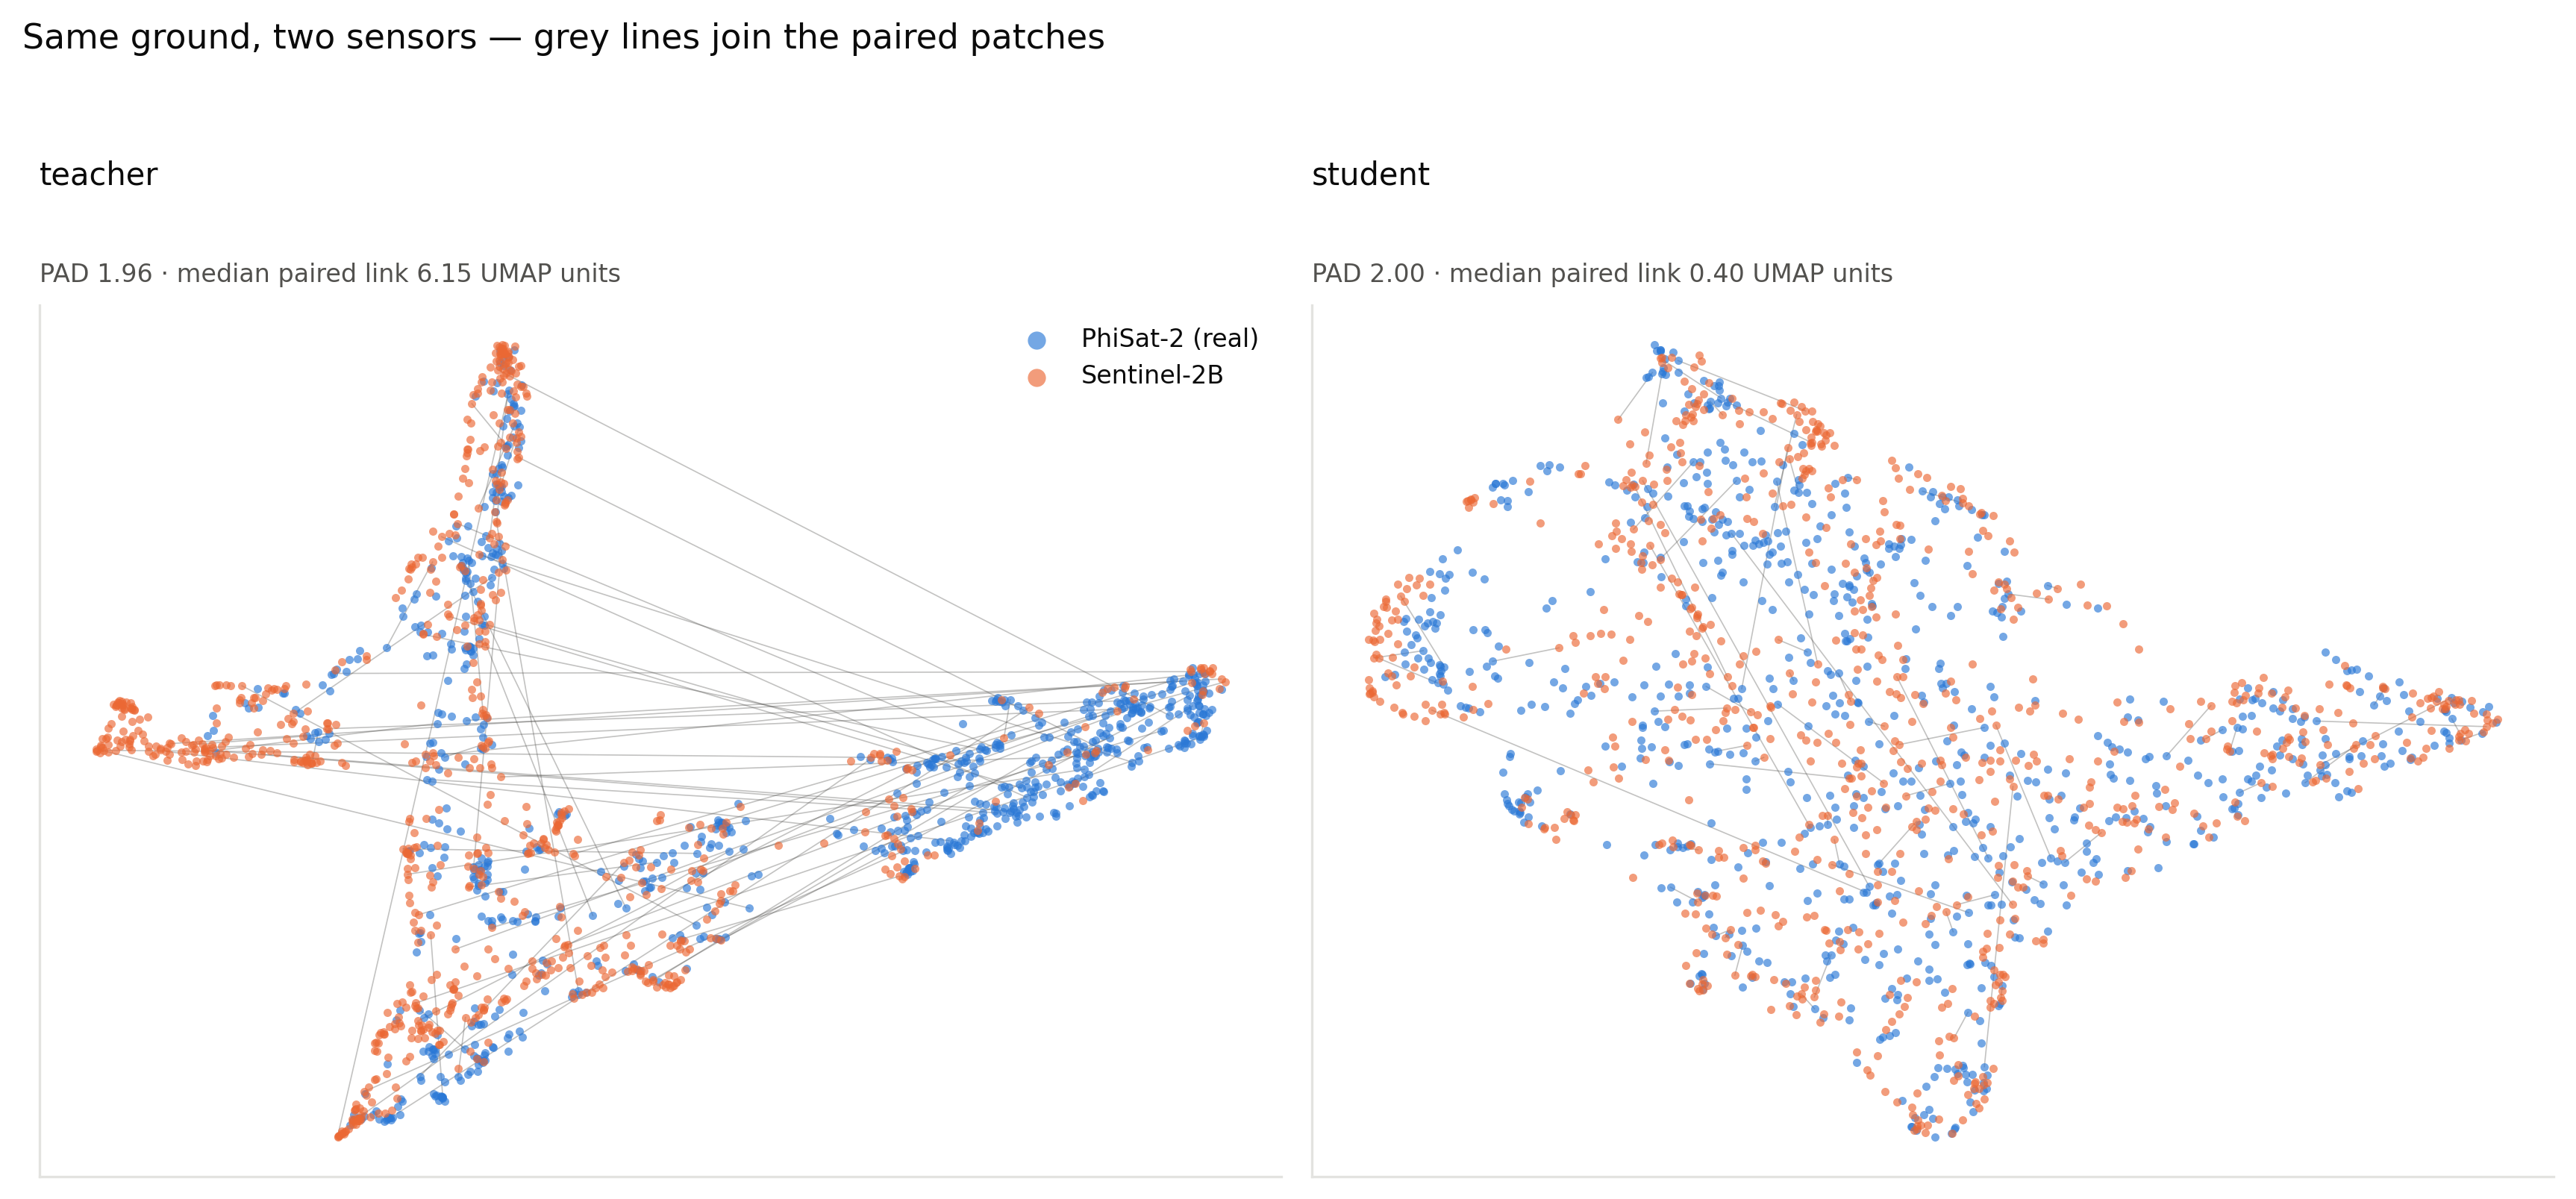
\includegraphics[width=\textwidth]{figures/fig_embeddings_paired.png}
    \caption{UMAP projection of pooled embeddings for $800$ co-registered test patches, teacher (left) and distilled student (right), each projected independently.
        Grey lines join the two sensor views of the same patch.
        In the teacher's space the paired views are far apart (median link $6.15$ units); in the student's they are effectively coincident ($0.40$ units).
    }
    \label{fig:embeddings-paired}
\end{figure}

A raw per-layer cosine-similarity check on the smaller TerraMind Tiny encoder, fine-tuned separately on real $\Phi$-sat-2 data as part of the earlier protocol described in Appendix~\ref{app:real-baseline}, is consistent with this picture (Figure~\ref{fig:cosine-sim-tiny}).
Similarity between paired Sentinel-2B and real-$\Phi$-sat-2 embeddings is near zero at the first block and rises through the middle of the network, mirroring the low-level-radiometry reading of the per-layer PAD result above.
This is a supplementary observation, on a different model scale and with a different measure than the analysis above (a raw cosine similarity in place of PAD), and we offer it as a consistency check rather than as a replication.

\begin{figure}[htbp]
    \centering
    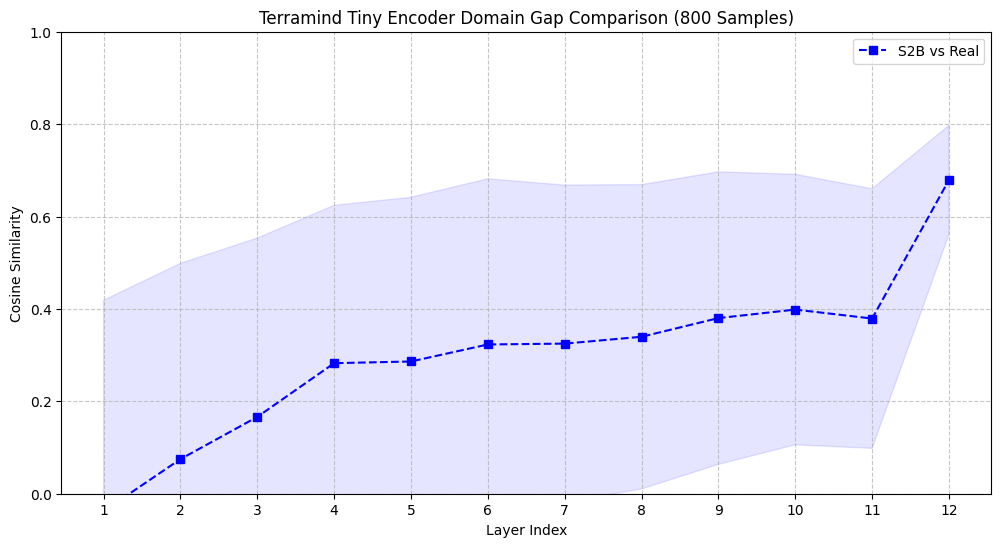
\includegraphics[width=0.85\textwidth]{figures/fig_cosine_sim_terramind.png}
    \caption{Per-layer cosine similarity between paired Sentinel-2B and real-$\Phi$-sat-2 patch embeddings from the TerraMind Tiny encoder, averaged over $800$ samples (shaded band: one standard deviation).
    }
    \label{fig:cosine-sim-tiny}
\end{figure}

\section{Degradation Factor effects on Downstream Task Gap (RQ1)}
\label{sec:ladder-results}

This section takes up the last part of RQ1, which asks which of the physical differences between the two instruments is the one that produces the gap.
This sub-question takes on the measurements above that established that a gap exists and that it is low-level in origin, and it asks which of the three low-level differences is responsible: radiometric noise, optical blur, or band misalignment.
The two instruments differ in their spectral response, their radiometric noise, their band registration and their ground sampling distance all at once, and no measurement on real pairs can separate those.
The simulated ladder of Section~\ref{sec:sen1floods-sim} makes the separation possible by degrading one factor at a time over identical scene content.
Three factors are varied over four severities each: sensor noise (SNR), optical blur (PSF), and band-to-band misalignment.
Table~\ref{tab:ladder-definition} gives the parameter values.
A severity axis common to all three is defined by setting level~4 to the operating point of the joint simulator configuration and halving the perturbation magnitude at each step down, so that a given level means the same fraction of full simulated degradation whichever factor is being varied.

\begin{table}[htbp]
    \centering
    \label{tab:ladder-definition}
    \begin{tabular}{lcccc}
        \toprule
        Level & Severity & SNR range  & PSF $\sigma$ (px) & Misalignment $\sigma$ (px) \\
        \midrule
        L1    & $0.125$  & $[40, 80]$ & $0.5$             & $1.25$                     \\
        L2    & $0.250$  & $[20, 40]$ & $1.0$             & $2.50$                     \\
        L3    & $0.500$  & $[10, 20]$ & $2.0$             & $5.00$                     \\
        L4    & $1.000$  & $[5, 10]$  & $4.0$             & $10.00$                    \\
        \bottomrule
    \end{tabular}
    \caption{The degradation ladder.
        Level~4 reproduces the joint simulator configuration; each step down halves the perturbation.
        SNR is drawn per scene from the stated range and the noise amplitude scales as its reciprocal, so the four ranges correspond to relative noise of $1/8$, $1/4$, $1/2$ and $1$.
        Blur and misalignment parameters are in resampled $4.75$\,m pixels.
    }
\end{table}

What we measure here is the domain gap proper: each model is trained once on the undegraded rung, and the resulting checkpoint is then evaluated on the test split of every rung, so the degradation only appears at inference, exactly as it would for a model trained on Sentinel-2 and deployed on $\Phi$-sat-2.
Three encoder configurations are compared: the distilled student with its encoder frozen and its decoder trained ($5.14$\,M of $9.86$\,M parameters trainable), TerraMind \texttt{base} under the same frozen-encoder protocol ($7.92$\,M of $94.25$\,M), and TerraMind \texttt{base} fine-tuned end to end.
Each configuration is run for three seeds using the same model checkpoint across all test splits.
Table~\ref{tab:ladder-domain-gap} reports the results.

\begin{table}[htbp]
    \centering
    \label{tab:ladder-domain-gap}
    \begin{tabular}{lccc}
        \toprule
                             & Distilled student           & TerraMind base            & TerraMind base                     \\
                             & (encoder frozen)            & (encoder frozen)          & (fine-tuned)                       \\
        \midrule
        Clean baseline (IoU) & $\mathbf{0.814} \pm 0.002$  & $0.739 \pm 0.057$         & $0.773 \pm 0.033$                  \\
        \midrule
        \multicolumn{4}{l}{\emph{Sensor noise (SNR)}}                                                                       \\
        \quad L1             & $-0.031 \pm 0.024$          & $+0.002 \pm 0.003$        & $-0.001 \pm 0.001$                 \\
        \quad L2             & $-0.114 \pm 0.099$          & $+0.003 \pm 0.006$        & $-0.004 \pm 0.002$                 \\
        \quad L3             & $-0.280 \pm 0.234$          & $-0.018 \pm 0.017$        & $-0.041 \pm 0.014^{\ast}$          \\
        \quad L4             & $\mathbf{-0.458} \pm 0.267$ & $-0.088 \pm 0.066$        & $-0.152 \pm 0.030^{\ast}$          \\
        \addlinespace
        \multicolumn{4}{l}{\emph{Optical blur (PSF)}}                                                                       \\
        \quad L1             & $-0.002 \pm 0.000^{\ast}$   & $-0.004 \pm 0.003$        & $0.000 \pm 0.000$                  \\
        \quad L2             & $-0.013 \pm 0.003^{\ast}$   & $-0.010 \pm 0.007$        & $0.000 \pm 0.001$                  \\
        \quad L3             & $-0.048 \pm 0.014^{\ast}$   & $-0.016 \pm 0.012$        & $0.000 \pm 0.003$                  \\
        \quad L4             & $-0.110 \pm 0.030^{\ast}$   & $-0.025 \pm 0.016$        & $\mathbf{-0.008} \pm 0.009$        \\
        \addlinespace
        \multicolumn{4}{l}{\emph{Band misalignment}}                                                                        \\
        \quad L1             & $-0.006 \pm 0.001^{\ast}$   & $-0.008 \pm 0.003^{\ast}$ & $-0.003 \pm 0.001^{\ast}$          \\
        \quad L2             & $-0.031 \pm 0.001^{\ast}$   & $-0.033 \pm 0.005^{\ast}$ & $-0.013 \pm 0.003^{\ast}$          \\
        \quad L3             & $-0.082 \pm 0.004^{\ast}$   & $-0.065 \pm 0.005^{\ast}$ & $-0.051 \pm 0.007^{\ast}$          \\
        \quad L4             & $-0.140 \pm 0.007^{\ast}$   & $-0.119 \pm 0.009^{\ast}$ & $\mathbf{-0.109} \pm 0.012^{\ast}$ \\
        \bottomrule
    \end{tabular}
    \caption{Domain gap across the degradation ladder: change in positive-class IoU relative to the undegraded test split, for a model trained only on undegraded data.
        Values are the mean over three seeds of the within-seed drop, $\pm$ one standard deviation of those drops; $^{\ast}$ marks a drop exceeding twice that deviation.
        The two model families are scored under different evaluation geometry (the student on $256$-pixel centre crops, TerraMind on full $1077$-pixel scenes), so the clean baselines are not comparable between columns and only the drops are.
    }
\end{table}

On undegraded data the distilled student is the strongest of the three, at $0.814$ IoU against $0.773$ for fine-tuned TerraMind and $0.739$ for frozen TerraMind.
The smaller student outperforming the foundation model on this clean task can be attributed to its stronger local representation, whereas TerraMind is a general-purpose encoder receiving only a task head and a fine-tuning pass.
The comparison of interest here is the response to degradation.

Band misalignment is the only factor that degrades every configuration significantly, monotonically, and by a similar amount.
Its full-severity cost varies only between $-0.109$ and $-0.140$ IoU across models that differ by an order of magnitude in trainable parameters and by architecture family, and it is the sole factor resolved at the mildest severity in all three columns, where a $1.25$-pixel shift already costs a small but reproducible amount.
Its seed-to-seed deviation is also the smallest in the table.
A perturbation whose cost is that insensitive to the model absorbing it is best read as a damage to the input signal, rather than as a weakness of any particular representation.
Band-to-band shifts corrupt precisely the cross-band relationships on which a water/land decision rests, and no amount of encoder capacity recovers an information that the shift has already destroyed.

Sensor noise produces the largest single degradation, but its magnitude is a property of the model rather than of the perturbation, and it is the least reproducible quantity in the table.
At full severity it costs the distilled student $-0.458$ IoU on average and fine-tuned TerraMind $-0.152$, a threefold difference that holds at every severity and stands in contrast to the near-constant cost of misalignment.
Neither the student's figure nor frozen TerraMind's ($-0.088$) is resolved at three seeds, because in both cases the seed-to-seed deviation of the drop ($0.267$ and $0.066$) is of the same order as the drop itself.

Optical blur is the least damaging factor in every configuration, but the three differ in how cleanly the effect is resolved.
For fine-tuned TerraMind it is indistinguishable from zero: four severities spanning a twenty-four-fold reduction in image gradient energy move the score by at most $0.008$ IoU.
For frozen TerraMind the response is monotone and uniformly negative but never clears the significance threshold, reaching $-0.025$ at full severity.
For the distilled student it is small but unambiguous, significant at all four severities with the tightest deviations in the table, rising from $-0.002$ to $-0.110$.
Blur is therefore real for the student and negligible for TerraMind, yet even for the student it remains the smallest of the three factors, costing a quarter of what noise costs at the same nominal severity.

This ordering settles the attribution question left open in Section~\ref{sec:rq1-results}, and it settles it in the same direction.
The factor that models a resolution difference, which is the optical blur, is the one that costs almost nothing, while the radiometric factor and the band-registration factor are the ones carrying the effect.
The per-layer PAD result located the gap in low-level radiometry rather than in semantics, and the ladder independently identifies the two low-level physical effects responsible, using a different task, a different measurement, and imagery in which scene content is held fixed by construction.
It also reinforces the point that the gap here is not resolution-driven, which is again the reverse of the emphasis found in related on-orbit work~\cite{du2025onorbitdemonstrationgeospatialfoundation}.

\begin{table}[htbp]
    \centering
    \label{tab:ladder-adaptation}
    \begin{tabular}{lccc}
        \toprule
        Factor at L4       & Trained clean, tested degraded & Trained and tested degraded & Recovered \\
        \midrule
        Sensor noise (SNR) & $-0.455$                       & $-0.072$                    & $84\%$    \\
        Band misalignment  & $-0.150$                       & $-0.051$                    & $66\%$    \\
        Optical blur (PSF) & $-0.128$                       & $+0.020$                    & all of it \\
        \bottomrule
    \end{tabular}
    \caption{Degradation seen at inference only, against degradation present during training as well, for the distilled student at full severity.
        The matched-condition column is a single seed and is not directly comparable in precision to the three-seed cross-condition column; it is reported to establish the size of the effect, which is large, not its exact value.
    }
\end{table}

One further comparison bears directly on what to do about these results.
Repeating the sweep with each model trained on the same degraded condition it is evaluated on, instead of on clean data, recovers most of the loss (Table~\ref{tab:ladder-adaptation}).
$84\%$ of the noise penalty and $66\%$ of the misalignment penalty disappear, and the blur ceases to be a penalty at all, since it scores marginally \emph{above} the clean baseline, in the manner of a mild augmentation.
The gap measured in Table~\ref{tab:ladder-domain-gap} is therefore largely an adaptation gap rather than an information-loss gap, at least for noise and blur.
Where the noise characteristics of the operating sensor are known in advance, which for a launched instrument they always are, simulating them during the training reclaims most of the achievable performance, and this without any domain-adaptation machinery at all.
Misalignment is again the exception: a third of its cost survives training on the degraded condition, which is consistent with reading it as genuine destruction of cross-band information.

Three limitations bound these results.
We vary the factors one at a time, whereas a real sensor pair presents all of them at once, and possibly interacting, so the ladder identifies which effects matter in isolation, and not how they compose.
The degradations are simulated, so the conclusion concerns the simulator's model of the instrument difference and not the instrument difference itself, and it is the absence of real labelled $\Phi$-sat-2 flood data (Section~\ref{sec:sen1floods-sim}) that makes this unavoidable.
Finally, the supervised U-Net baseline is not included in Table~\ref{tab:ladder-domain-gap}, so these results characterise the distilled and foundation-model encoders but do not establish whether distillation itself changed robustness relative to training on the target sensor directly.

\wip{Two further pieces of this evaluation are prepared but not yet included: a latent-space view of how the ladder displaces the U-Net's representation, and the corresponding domain-gap metrics of Section~\ref{sec:gap-measurement} computed per rung.
    Both are expected to test the same attribution from the representation side rather than the task side, and the reading above should be revisited if they disagree with it.
}

\section{Sensor Adaptivity in the Distilled Student (RQ2)}
\label{sec:rq2-results}

The distilled student inverts every one of these measurements.
The paired cosine similarity rises from $0.098$ to $0.948$, and the probe transfer from $33\%$ to $97\%$ ($0.663 \rightarrow 0.646$), which means that a classifier fitted on the student's Sentinel-2 features is very nearly as accurate on its $\Phi$-sat-2 features.
In Figure~\ref{fig:embeddings-paired} the paired links collapse to $0.40$ UMAP units, a fifteen-fold reduction.
The downstream consequence is visible in the right panel of Figure~\ref{fig:dsbn-vs-baseline}.
The accuracy of the student on the two sensors converges on parity: on the test split it scores $0.4454$ on $\Phi$-sat-2 against $0.4417$ on Sentinel-2, which is a residual difference of $-0.004$ mIoU, and this against a teacher whose representation does not usefully transfer at all.
Table~\ref{tab:invariance} collects the three measures side by side.

\begin{table}[htbp]
    \centering
    \label{tab:invariance}
    \begin{tabular}{lcc}
        \toprule
        Measure                                      & TerraMind teacher & Distilled student \\
        \midrule
        Paired cosine similarity                     & $0.098$           & $\mathbf{0.948}$  \\
        Median paired link (UMAP units)              & $6.15$            & $\mathbf{0.40}$   \\
        Probe: Sentinel-2 $\rightarrow$ Sentinel-2   & $0.754$           & $0.663$           \\
        Probe: Sentinel-2 $\rightarrow$ $\Phi$-sat-2 & $0.250$           & $\mathbf{0.646}$  \\
        Probe transfer retention                     & $33\%$            & $\mathbf{97\%}$   \\
        \addlinespace
        IoU($\Phi$-sat-2) $-$ IoU(Sentinel-2), test  & ---               & $\mathbf{-0.004}$ \\
        \bottomrule
    \end{tabular}
    \caption{Sensor invariance of the teacher and the distilled student, over $800$ co-registered test patches.
        Paired cosine and probe transfer compare the two sensor views of the \emph{same} ground.
        Probe transfer fits a linear classifier on Sentinel-2 embeddings and applies it to $\Phi$-sat-2 embeddings; retention is the ratio of the two accuracies.
        The IoU difference is measured on the full test split rather than on the $800$-patch embedding sample.
    }
\end{table}

\wip[Decide how to frame the probe row that cuts against the student.]{%
    To write: a remark on the one row that cuts against the student.
    The teacher is the stronger encoder \emph{within} Sentinel-2 ($0.754$ against $0.663$ same-domain probe accuracy), and its advantage only disappears once the probe is asked to cross the sensor gap.
    This can be framed either as a limitation of the student, or as the precise statement of what the distillation bought.
}

One measurement in this set behaves counter-intuitively, and it illustrates a real trap in evaluating this class of method.
The raw PAD is maximal for the student ($2.000$, against $1.955$ for the teacher), which means that a linear probe separates the two domains perfectly.
This is an artefact of the mechanism itself, since the domain-specific normalization gives each sensor its own affine transform.
A constant per-channel offset distinguishes the domains by construction, and a linear probe finds it trivially regardless of how well the semantic content is aligned.
Standardising each domain on its own statistics removes exactly the first and second moments that a per-domain affine can express, and it drops the probe to chance for both models.
Figure~\ref{fig:pad-decision} shows the underlying quantity: in the raw setting the two domains' probe scores are separated by an empty margin, and after per-domain standardisation they collapse onto one another.

PAD is therefore not a valid instrument for a model that carries a domain-specific normalization, even though it is scale-free and hence otherwise well suited to comparing representations of different dimensionality.
The probe transfer, which asks the functional question directly, is the appropriate measure here, and it is the one we report above.

\wip{The same caution applies in weaker form to the two measures this section does rely on.
    Domain-specific normalization aligns each domain's first and second moments by construction, and both paired cosine similarity and probe transfer are sensitive to that alignment, so some part of the improvement reported above may share an origin with the PAD artefact instead of reflecting semantic alignment alone.
    Recomputing both measures on a student trained with shared normalization, and after standardising each domain on its own statistics, is in progress and is the check that would settle how much of the gain is representational.
    Until it completes, the magnitude of the invariance improvement should be read as an upper bound, though the direction of the effect is not in doubt: the teacher's representation does not transfer across the sensor pair at all, and the student's does.
}

\begin{figure}[htbp]
    \centering
    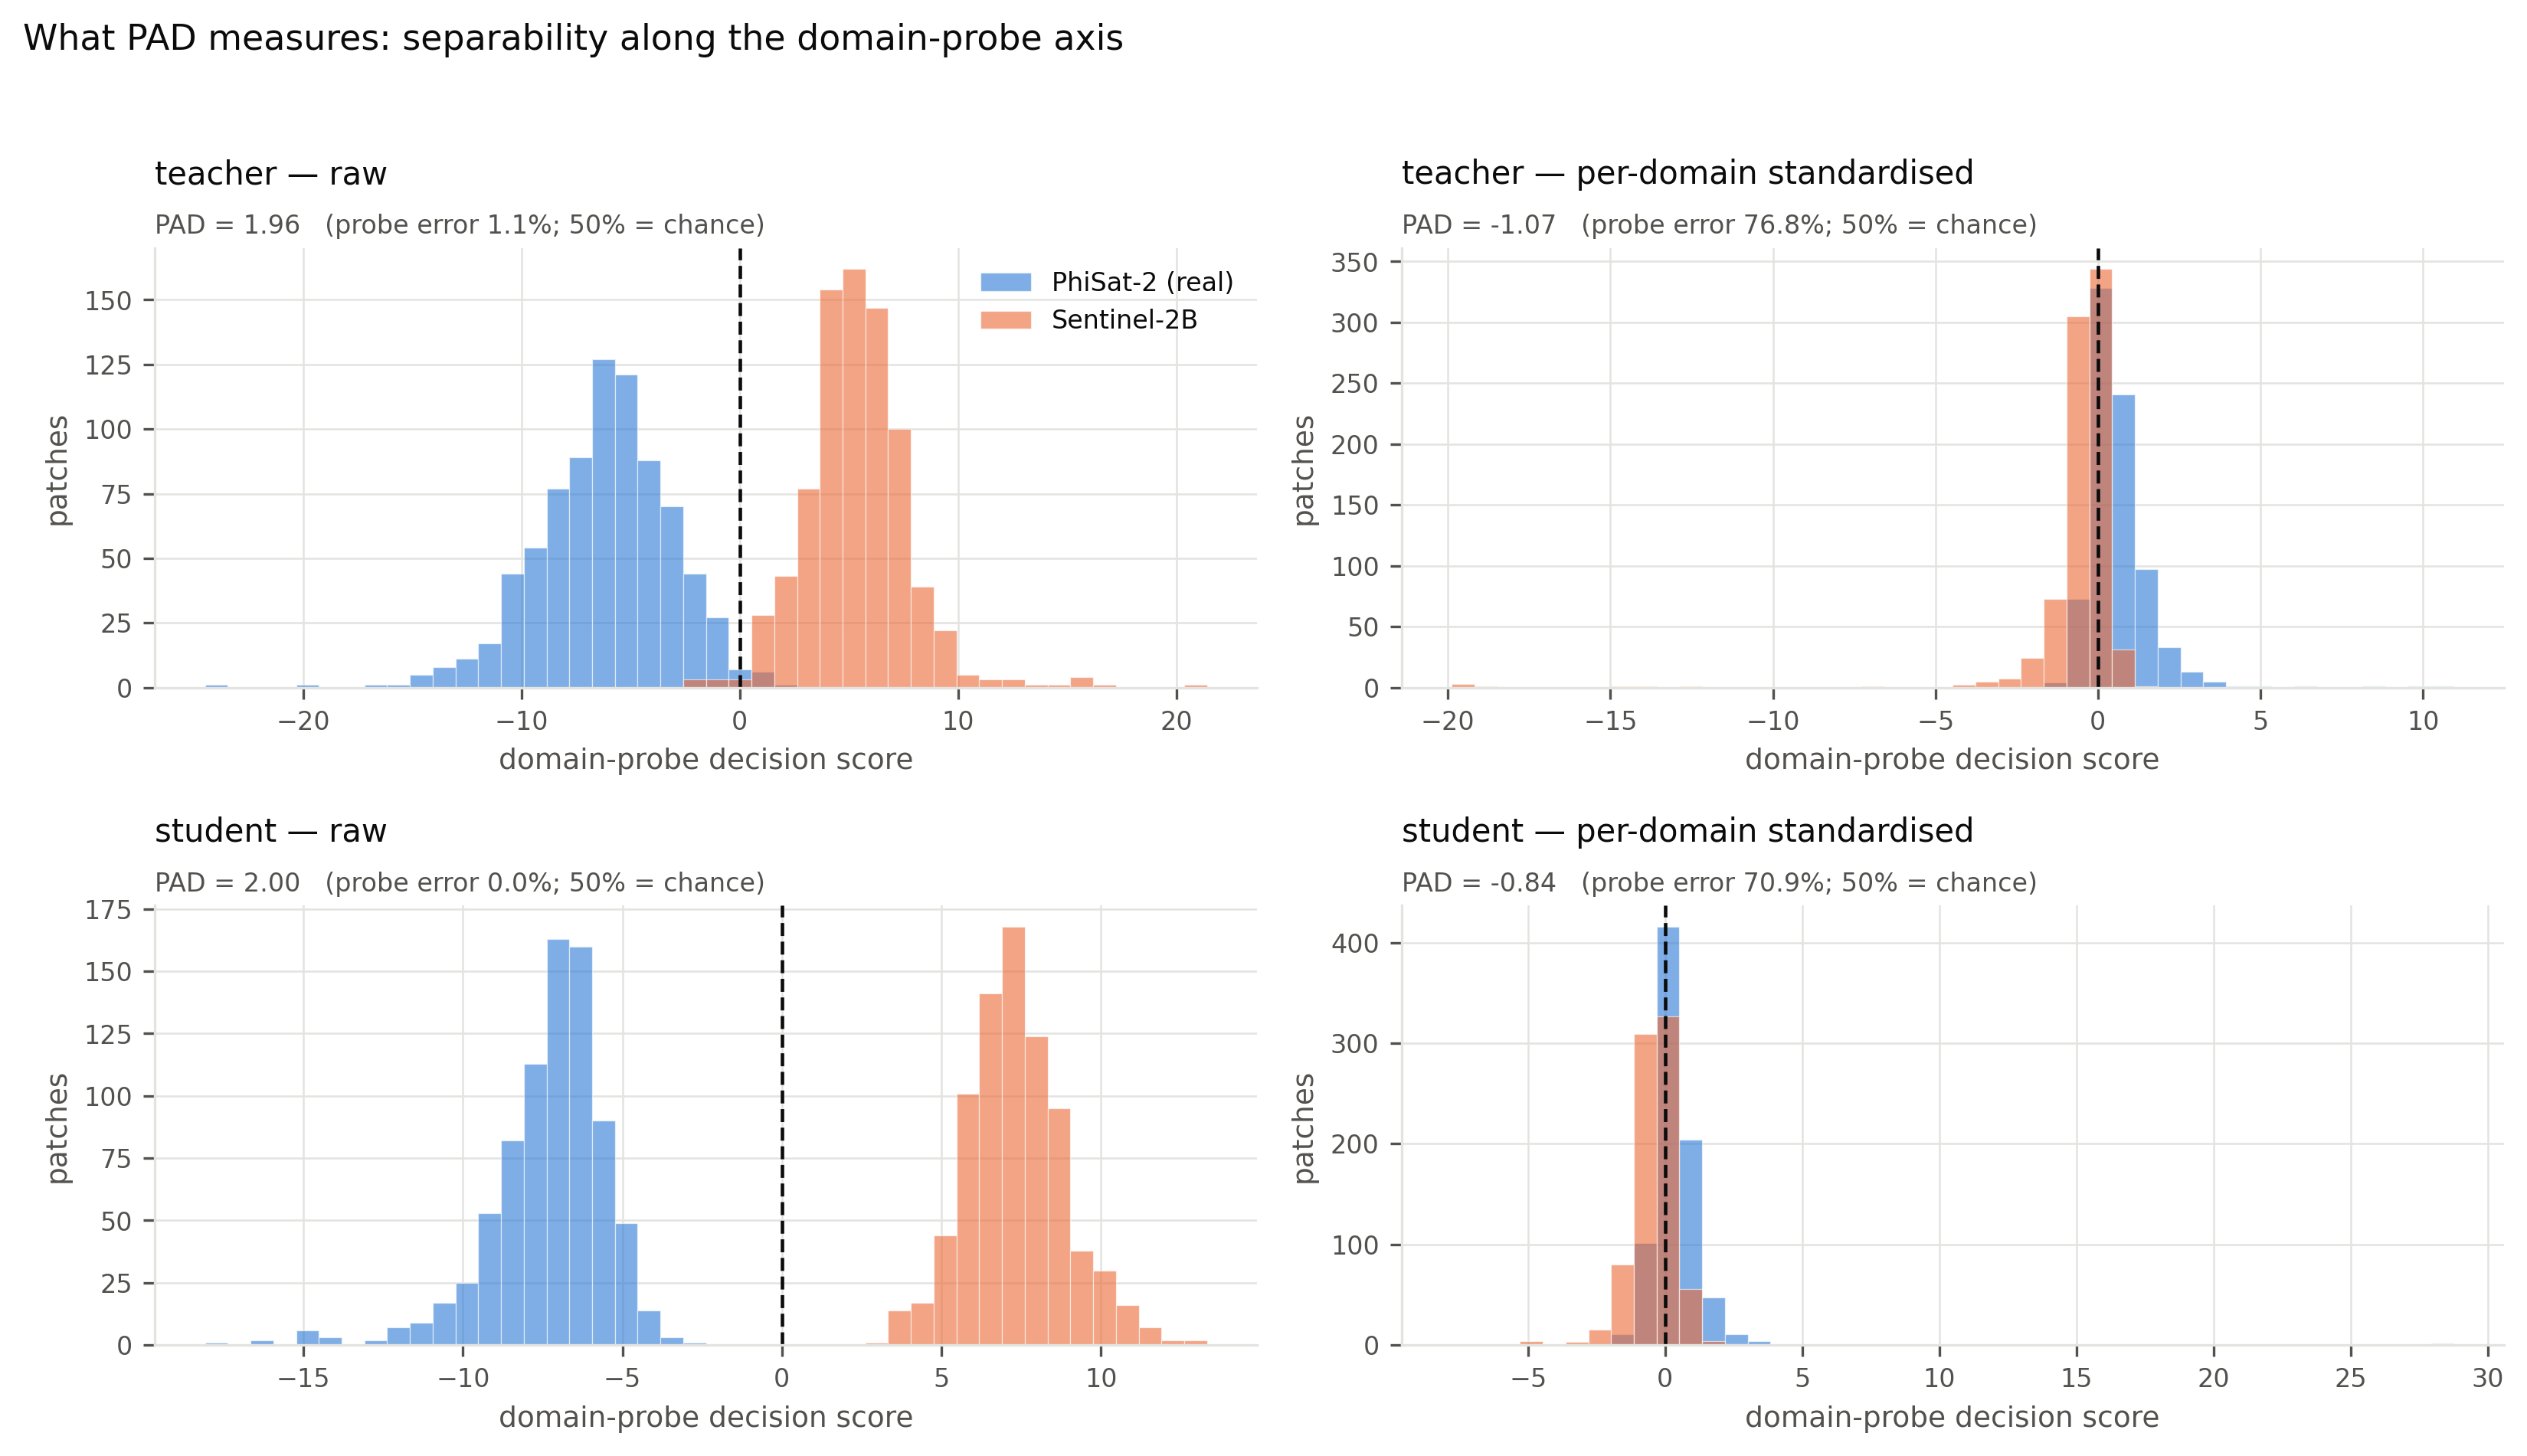
\includegraphics[width=\textwidth]{figures/fig_pad_decision_scores.png}
    \caption{Distribution of the domain probe's out-of-fold decision score, the quantity from which PAD is computed.
        Separated modes imply a probe that never errs (PAD $\rightarrow 2$); overlapping modes imply chance (PAD $\rightarrow 0$).
        After standardising each domain on its own statistics (right column) the separability vanishes for both models, showing that all of it was per-channel mean and scale, not representational structure.
    }
    \label{fig:pad-decision}
\end{figure}

This result should be stated precisely.
With a domain-specific normalization, the encoder is domain-adaptive rather than domain-invariant: the convolutional weights are shared, the normalization statistics are not, and the target-sensor branch has to be selected at inference.
The defensible claim is therefore that after a per-domain normalization, the structure learned on the source sensor is $97\%$ readable on the target one.
That is weaker than a single sensor-agnostic encoder, but it is the property that an on-board deployment actually requires, since the acquiring instrument is always known.

\section{Distillation Against a Supervised Baseline (RQ3)}
\label{sec:rq3-results}

Sensor adaptivity is only useful if it buys an accuracy that a simpler method would not.
Our control is a student of identical architecture, trained directly on labelled $\Phi$-sat-2 with no teacher, no second sensor and no distillation, and holding constant the split, the normalization, the augmentation, the task loss, the optimiser, the schedule and the early-stopping criterion (Table~\ref{tab:hyperparameters}).

At a budget of $10{,}000$ labelled patches the distilled student reaches $0.4607$ best validation mIoU against the baseline's $0.3989$, a margin of $0.0618$ (Table~\ref{tab:main-results}).
Figure~\ref{fig:dsbn-vs-baseline} shows the shape of that margin: the baseline is ahead for roughly the first twenty-five epochs, then the two curves cross, and the distilled run separates and keeps climbing after the baseline has flattened.
Averaged over the $71$ epochs the two runs share, the distilled student leads by $0.0161$ mIoU and is ahead in $49$ of them.

\wip[Settle the framing of the late overtake against the curves.]{%
    To write: an interpretation of \emph{why} the distilled run overtakes late rather than early.
    These runs do not establish the mechanism.
    The candidate explanations are that the teacher's signal becomes most useful once the student has enough capacity committed to the easy classes, or simply that the two-branch arm sees twice the supervision per epoch and therefore trails on wall-clock but not on epochs.
}

The distilled run had not converged.
Its best epoch is the $89$th of the $101$ it ran, and it exhausted the full budget without ever triggering the early stopping, so $0.4607$ should be read as a lower bound on what this configuration reaches.
The baseline, by contrast, early-stopped at epoch $80$.

The per-class results (Figure~\ref{fig:per-class}) show that the gain is a broad one, and not concentrated in a single class.
Distillation is ahead on nine of the eleven classes, most markedly on mangroves ($+0.144$), grassland ($+0.135$), moss/lichen ($+0.115$), tree cover ($+0.100$) and cropland ($+0.099$).
It is behind on permanent water ($-0.019$) and level on shrubland ($-0.002$).
The frequency-weighted IoU moves in the same direction as the macro average ($0.523$ against $0.454$), so this result is not an artefact of the rare-class weighting introduced in Section~\ref{sec:configuration}.

\wip[Decide how much weight the two classes where the baseline wins deserve.]{%
    To write: the per-class discussion.
    Permanent water is the only class where the undistilled baseline is meaningfully ahead ($-0.019$), with shrubland level, and it is spectrally distinctive and not rare enough for the class weighting to be doing the work.
    This needs a sentence on whether that pattern is meaningful, or whether it sits within the per-class noise of a single seed.
}

Two costs qualify this result.
The distillation requires $7.9$ minutes per epoch against the $3.3$ of the baseline, which is a factor of $2.4$, and it is dominated by the forward pass of the frozen teacher and by the second student branch.
At a fixed compute budget rather than a fixed epoch count, the comparison would therefore be much closer.
Separately, the teacher reaches $0.6351$ mIoU on Sentinel-2 while the student reaches $0.4454$ on $\Phi$-sat-2, so roughly $0.19$ mIoU of the teacher--student gap remains unclosed.
That residual is a compression gap rather than a domain gap, since Section~\ref{sec:rq2-results} shows that the student performs almost identically on the two sensors, so what separates it from the teacher is its capacity and its initialisation.

\begin{table}[htbp]
    \centering
    \label{tab:main-results}
    \begin{tabular}{llccc}
        \toprule
        Labels                                                        & Method              & Val.\ mIoU        & Test mIoU         & Cost (h)       \\
        \midrule
        $10{,}000$                                                    & KD + DSBN           & $\mathbf{0.4607}$ & $\mathbf{0.4454}$ & $13.3$         \\
        $10{,}000$                                                    & Supervised baseline & $0.3989$          & $0.3782$          & $\mathbf{4.4}$ \\
        \addlinespace
        $1{,}000$                                                     & KD + DSBN           & $0.2679$          & $0.2635$          & $2.2$          \\
        $1{,}000$                                                     & Supervised baseline & $\mathbf{0.2916}$ & $\mathbf{0.2707}$ & $\mathbf{0.6}$ \\
        \midrule
        \multicolumn{2}{l}{TerraMind teacher (Sentinel-2, reference)} & ---                 & $0.6351$          & ---                                \\
        \bottomrule
    \end{tabular}
    \caption{Main results on the LULC task.
        Validation mIoU is the best epoch, on the fixed $1{,}000$-patch validation split shared by every run; because the splits are nested prefixes of one shuffled ordering, the two label budgets are evaluated on the identical patches.
        Test mIoU is on the full $25{,}323$-patch test split.
        Cost is total wall-clock for the run.
    }
\end{table}

Both test scores in Table~\ref{tab:main-results} are measured on the full $25{,}323$-patch split.
The $10{,}000$-label baseline was originally evaluated on a $997$-patch subset, before the evaluation split was decoupled from the training budget (Section~\ref{sec:measurement-pitfalls}); its stored checkpoint was re-evaluated on the full split for this table, which moved its score from $0.3902$ to $0.3782$ and required no retraining.
The size of that shift is worth noting on its own: the same frozen teacher scores $0.5788$ on the $997$-patch subset and $0.6351$ on the full split, so subset-to-subset differences of this magnitude are not negligible at all, and no number coming from the two evaluation regimes should be compared directly.

\begin{figure}[htbp]
    \centering
    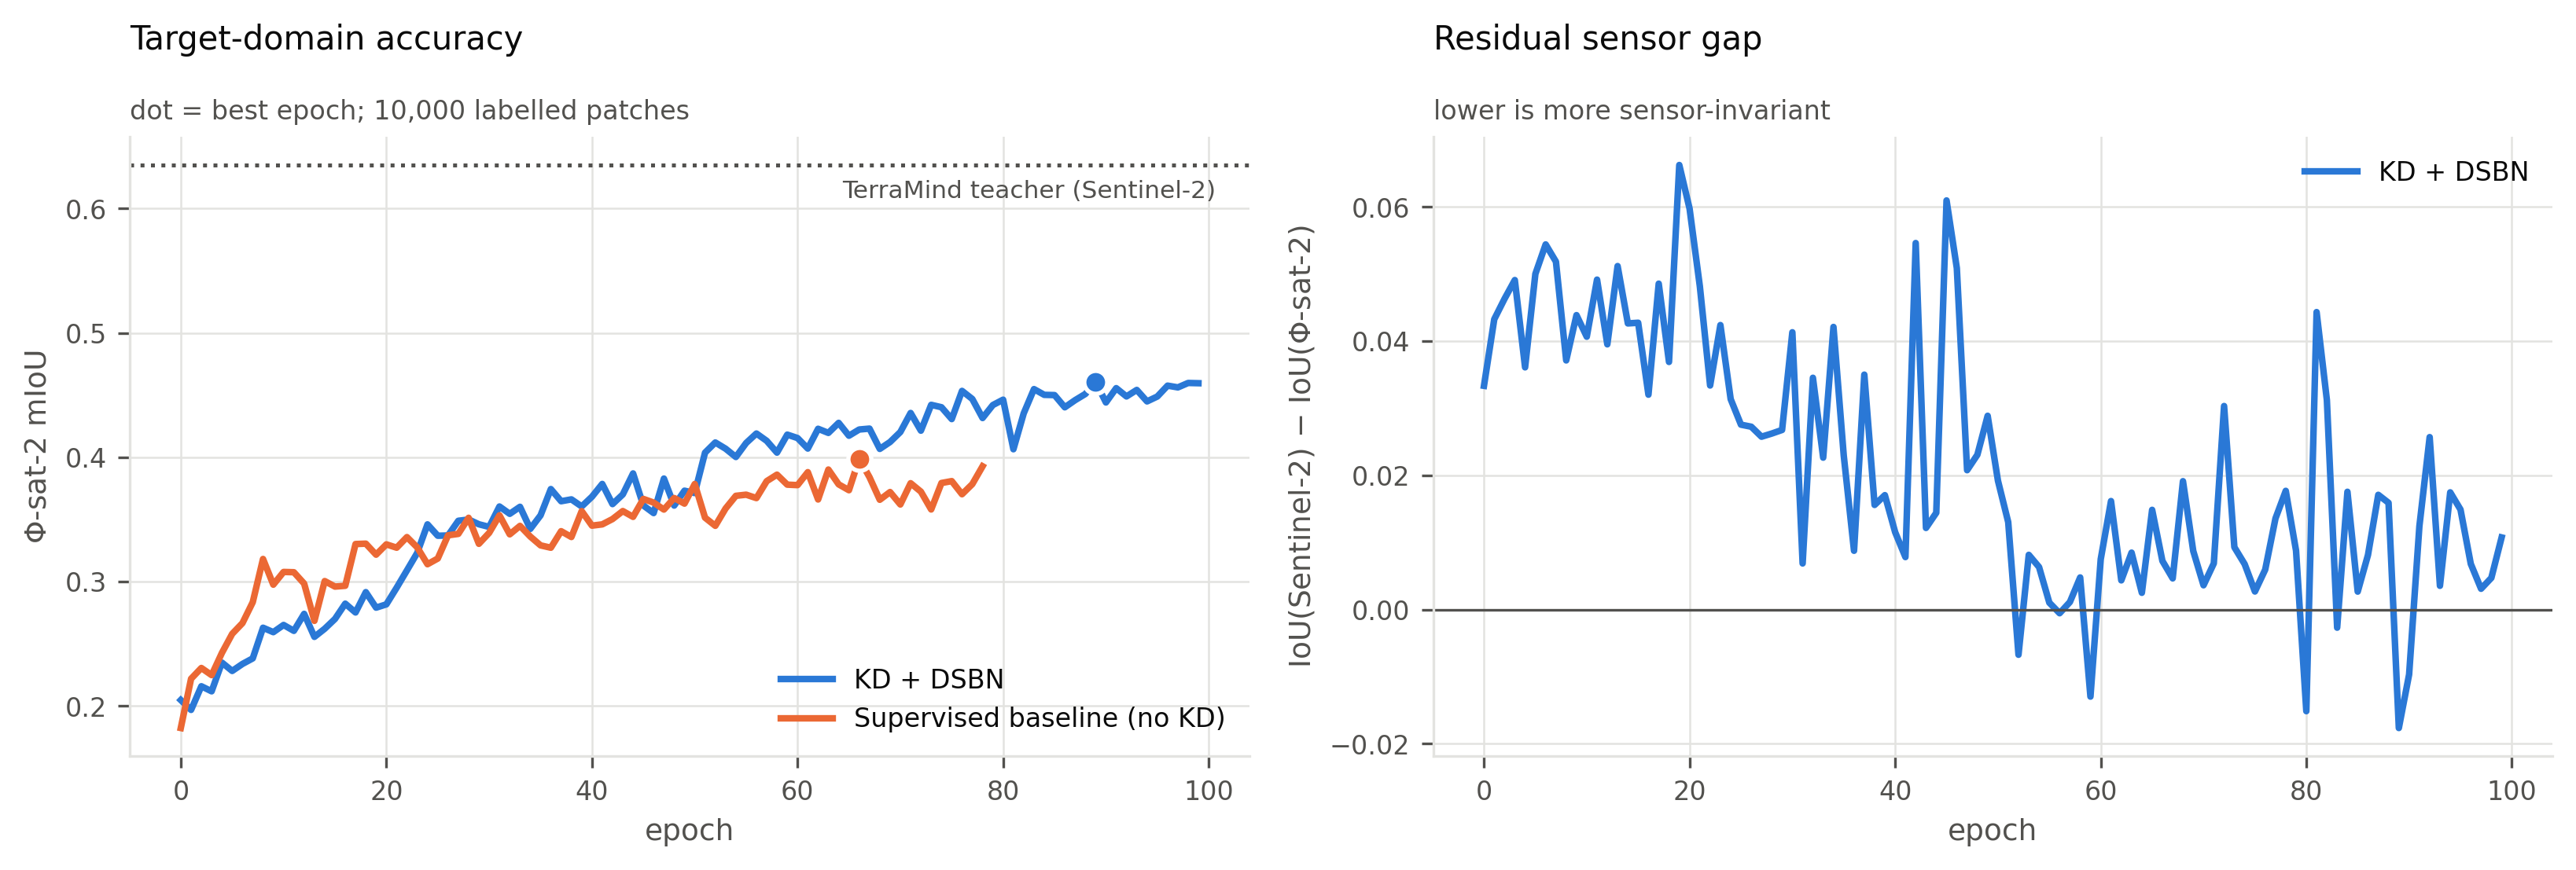
\includegraphics[width=\textwidth]{figures/fig_dsbn_vs_baseline.png}
    \caption{Left: $\Phi$-sat-2 validation mIoU over training at $10{,}000$ labelled patches, with the best epoch marked; the dotted line is the teacher's Sentinel-2 accuracy.
        Right: the residual accuracy difference between the two sensors for the distilled student, which crosses zero around epoch $55$ and oscillates about it thereafter.
    }
    \label{fig:dsbn-vs-baseline}
\end{figure}

\begin{figure}[htbp]
    \centering
    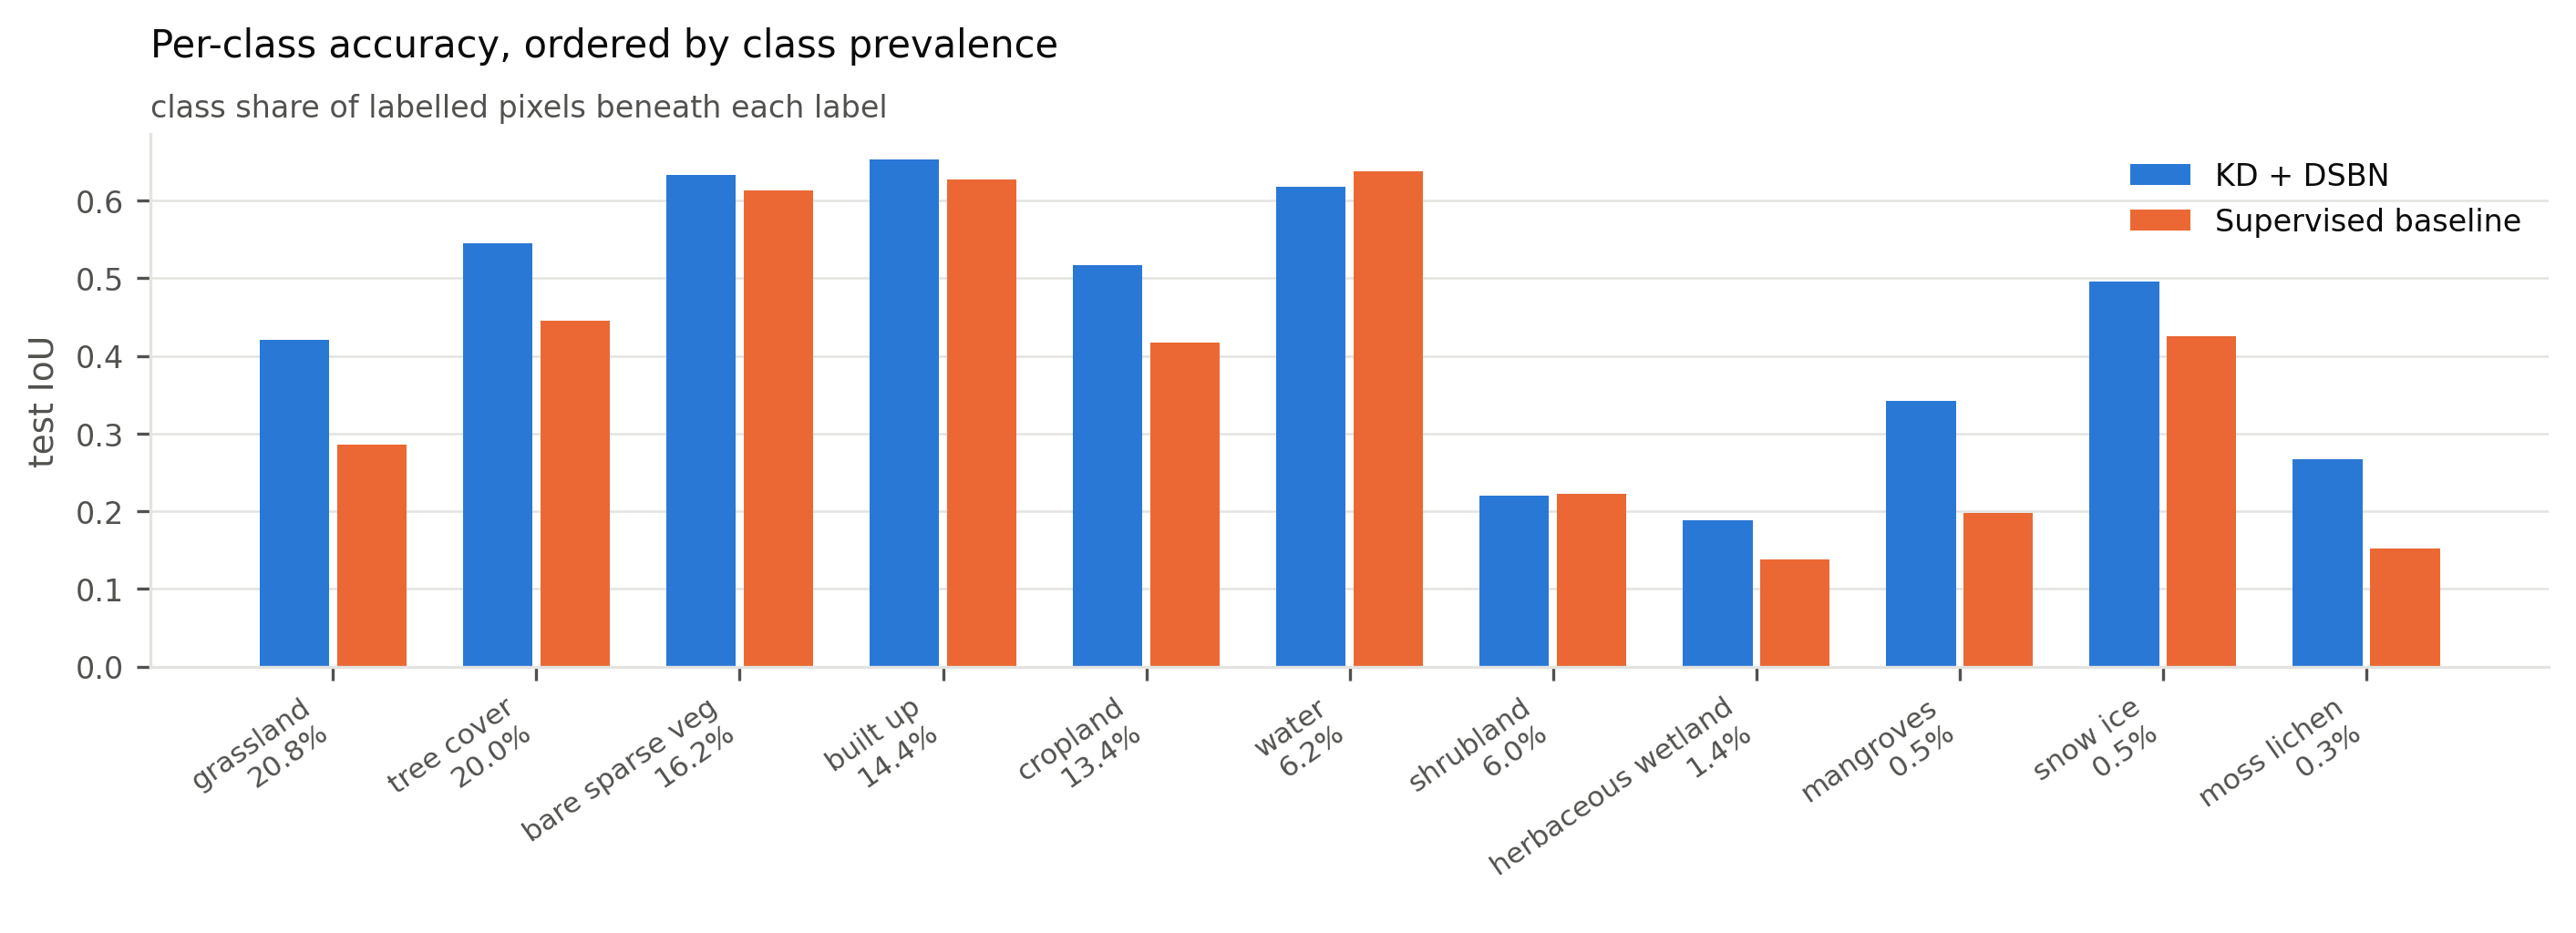
\includegraphics[width=\textwidth]{figures/fig_per_class_dsbn.png}
    \caption{Per-class test IoU at $10{,}000$ labelled patches, ordered by class prevalence, with each class's share of labelled pixels beneath its label.
        Neither model leaves any class unlearned, which unweighted cross-entropy did for four of them (Section~\ref{sec:configuration}).
    }
    \label{fig:per-class}
\end{figure}

\section{Advantage Reversal on Small Label Budget}
\label{sec:label-crossover}

KD and UDA are usually motivated by a label scarcity in the target domain~\cite{kouw2019introductiondomainadaptationtransfer}, so we would expect the advantage above to grow as the target labels are removed, however the opposite is observed.
At $1{,}000$ labelled patches the supervised baseline is ahead by every measure: best validation mIoU $0.2916$ against $0.2679$, test mIoU $0.2707$ against $0.2635$, and on matched epochs the distilled student leads in only $8$ of the $58$ epochs both runs share.
It also does so at roughly a third of the cost, and this even though the distilled run had the larger budget available to it: it used its full hundred epochs without ever triggering the early stopping, while the baseline stopped at sixty-seven.
Figure~\ref{fig:label-crossover} shows the crossover; both budgets are evaluated on the identical fixed $1{,}000$-patch validation split, so the two points are directly comparable.

The reversal is consistent across every measure reported (best validation mIoU, test mIoU, and the epoch-by-epoch lead), but the two ends of the crossover are not equally well resolved.
At $10{,}000$ labels the margin ($0.0543$ validation mIoU) is larger than the epoch-to-epoch variance noted at the start of this chapter; at $1{,}000$ labels it is not ($0.0237$ validation, $0.0072$ test), and the baseline's advantage at the small budget therefore rests mainly on the consistency of the epoch-by-epoch lead, not on the size of the final gap.
Replication across seeds is required before the small-budget end of the crossover can be treated as established, and that is the appropriate reading of it here.
A plausible reading is that the distilled configuration carries substantially more machinery, which is a second forward pass, doubled normalization parameters, and a distillation term pulling toward a teacher that is itself imperfect at $0.5788$ mIoU, and that below a certain label threshold, the cost of all this machinery exceeds the value of the teacher's signal.
This is offered as a hypothesis: with two budgets the crossing point is bracketed but not located, and intermediate budgets would be required to characterise it.

\begin{figure}[htbp]
    \centering
    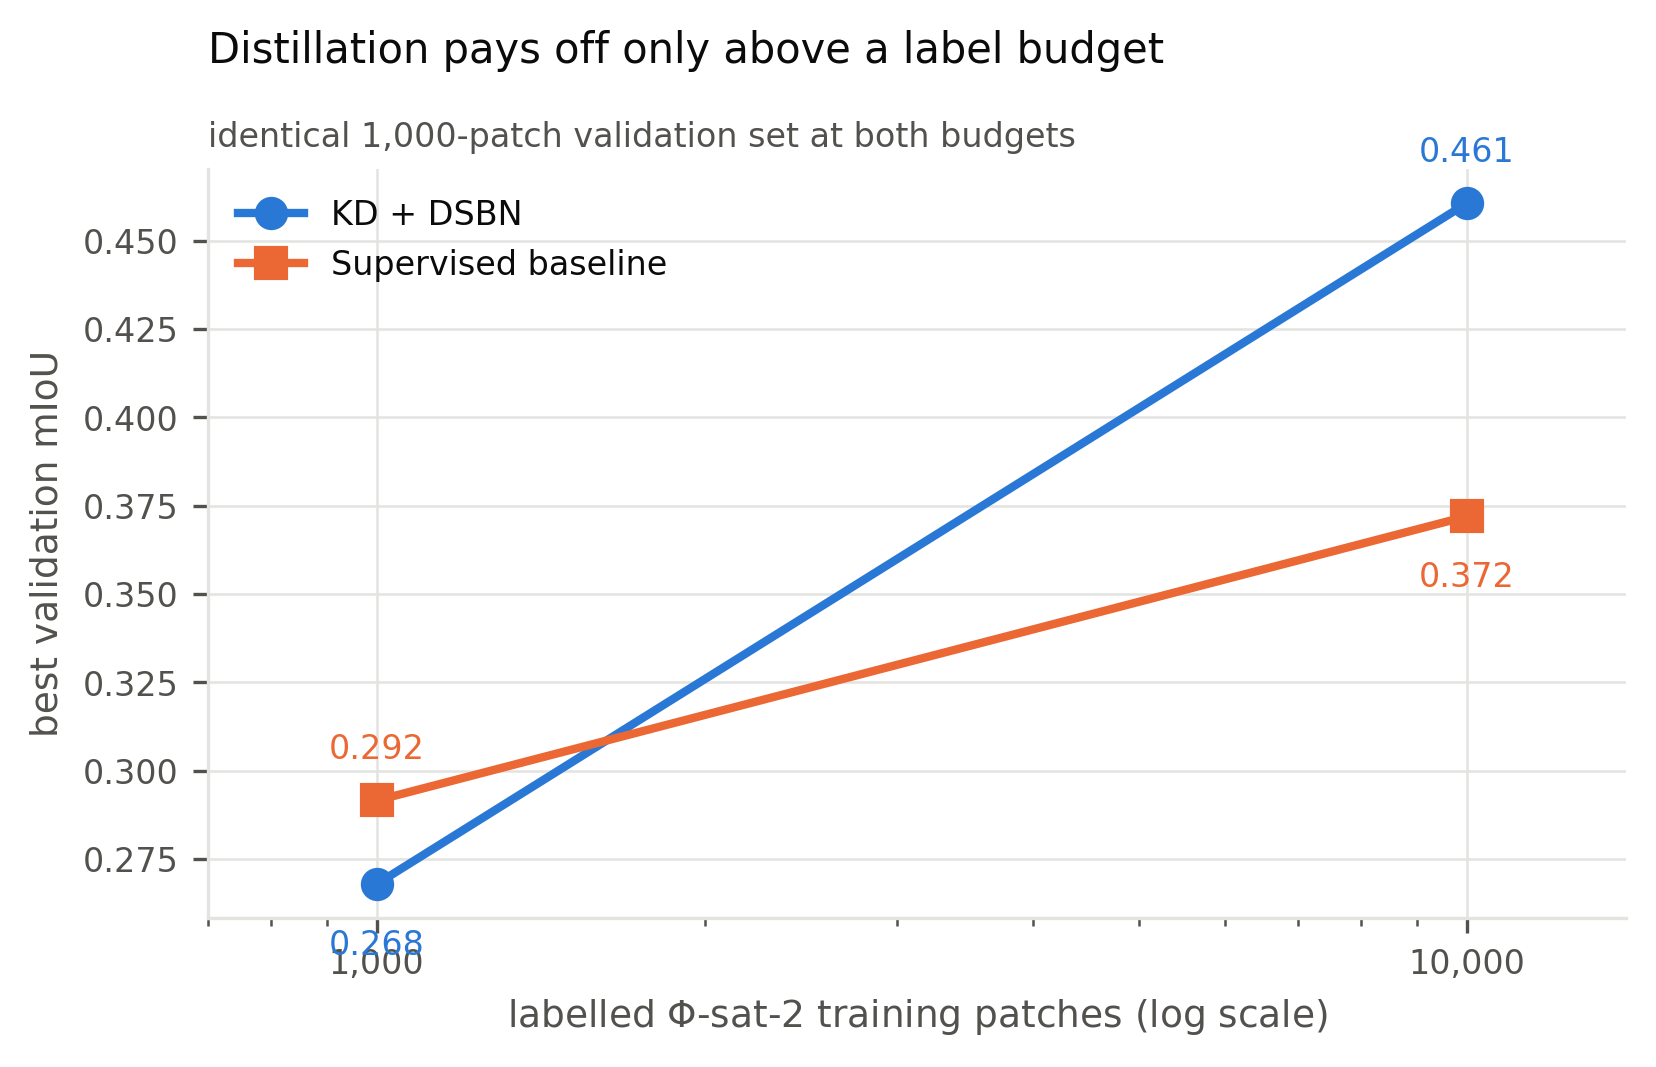
\includegraphics[width=0.72\textwidth]{figures/fig_label_crossover.png}
    \caption{Best validation mIoU against labelled training budget.
        The two methods cross: distillation is worse at $1{,}000$ labelled patches and better at $10{,}000$.
        Both budgets share the same fixed validation split.
    }
    \label{fig:label-crossover}
\end{figure}

\section{Discussion}
\label{sec:discussion}

\subsection{Domain-specific normalization contribution}

The improvement brought by the domain-specific normalization is larger than what a pure domain-alignment effect would predict, and its shape is informative: the accuracy on the source sensor improved by a margin similar to the one on the target ($+0.116$ against $+0.185$ test mIoU relative to the preceding configuration).
A mechanism that only aligned domains should have improved the target branch alone.
The most likely explanation is the train/test normalization inconsistency described in Section~\ref{sec:configuration}: the prior configurations were evaluated through a normalization path that the encoder had never been optimised under, which depressed the two branches at once.
On that reading, part of what is reported here as a domain-adaptation gain is the repair of a latent defect in the two-branch training scheme.
That caveat does not diminish the practical result, but it does bear on how much of it should be attributed to DA.

\subsection{Measurement pitfalls}
\label{sec:measurement-pitfalls}

Two artefacts we encountered during this work are worth recording, since both of them would silently corrupt a comparison of exactly this kind.

First, the macro-averaged mIoU implemented by standard libraries excludes classes with zero union from its average, so its denominator depends on which classes a given model happens to predict.
Where a rare class is absent from a small evaluation split, two models are then averaged over a different number of classes and their mIoU values are simply not comparable.
This effect inflated an apparent advantage by roughly a factor of three in an early version of the label-budget experiment.
All results in this chapter are reported on a fixed denominator over all eleven classes.

Second, and relatedly, an evaluation split sized as a fixed fraction of the training split makes a label-scarcity study vary its measurement and its treatment at the same time.
At the smallest budget, this left us with one hundred evaluation patches, in which the rarest class does not occur at all.
We therefore hold the evaluation splits fixed and independent of the training budget throughout.

\subsection{Limitations}
\label{sec:limitations}

All experiments use at most $10{,}000$ of the $202{,}582$ available training patches, under $5\%$, so the crossover of Section~\ref{sec:label-crossover} is characterised entirely within the low-data regime, and the ranking at full scale is untested.
Single seeds are used everywhere except the degradation-ladder evaluation of Section~\ref{sec:ladder-results}, so apart from that section no result in this chapter is supported by independent replication; epoch-to-epoch validation variance is of the order of $0.02$ mIoU, and differences below roughly $0.03$, which includes the small-budget end of the crossover in Section~\ref{sec:label-crossover}, are consequently not resolved.
Two further controls are outstanding at the time of writing: a shared-normalization distillation run isolating the contribution of domain-specific normalization (Section~\ref{sec:configuration}), and a recomputation of the invariance measures under shared and per-domain-standardised normalization (Section~\ref{sec:rq2-results}).
The student is trained from a random initialisation because no pre-trained weights exist for this backbone, and this plausibly accounts for a substantial share of the remaining $0.15$ mIoU gap to the teacher, and it confounds any claim that this gap would be attributable to a domain shift.
Finally, the work is scoped to a single sensor pair, so the finding that the gap is radiometric rather than resolution-driven (Section~\ref{sec:rq1-results}) should not be generalised beyond it.

\subsection{Interpretation of the flood-robustness result}
\label{sec:discussion-comparison}

\wip{The flood-segmentation evaluation is only partially complete at the time of writing, and the scope of what follows should be read accordingly.
    The robustness assessment across the simulated degradation ladder (Section~\ref{sec:ladder-results}) covers TerraMind, in both frozen and fine-tuned configurations, and the distilled student; the supervised U-Net baseline has not been run across the ladder, so no statement is yet possible about whether distillation changed flood-task robustness relative to training on the target sensor directly.
    The invariance and label-budget findings above therefore still rest on the LULC task alone, and no claim is made yet about whether they carry over to flood segmentation.
}

The mild flood-IoU degradation observed for the teacher across the simulated degradation ladder (Section~\ref{sec:ladder-results}, at worst $-0.152$ IoU under full-severity noise and $-0.008$ under full-severity blur) is not unique to this thesis.
Du et al.~\cite{du2025onorbitdemonstrationgeospatialfoundation} independently report that flood detection was anomalously robust to the sensor domain gap on Kanyini, in contrast to an approximately $47\%$ drop in cloud-detection performance on the same platform.
Two independent studies therefore observe the same pattern, and a plausible explanation is that the strong near-infrared absorption contrast of water survives the sensor noise and the band mismatch much better than the texture-dependent and boundary-dependent cues that cloud detection or general land-cover classification rely on.
Flood segmentation may then understate the severity of the domain-gap problem, and this is part of why we adopted the LULC task as the primary benchmark.

\subsection{Positioning with \texorpdfstring{$\Phi$}{Phi}satNet}

$\Phi$satNet (Section~\ref{sec:phisatnet-background}) reports that a purpose-built, non-transformer model trained from scratch on a mission-specific corpus matches or exceeds unconstrained transformer-based GeoFMs on several on-board tasks~\cite{phisatnet}.
This raises a reasonable objection: if a bespoke lightweight model already performs well without any of the machinery developed here, what is gained by adapting TerraMind instead?

The results of Section~\ref{sec:label-crossover} sharpen that question without settling it.
The answer this thesis offers is a label-efficiency bet: that a large-scale multi-modal pre-training generalises to new $\Phi$-sat-2 tasks with fewer labels than a narrower and curated pre-training suite requires.
The crossover we measure here shows that such a bet is budget-dependent, in a way that has to be quantified rather than assumed.
A matched few-shot comparison against $\Phi$satNet on a shared task and label budget remains the appropriate test and has not been run.

\subsection{Practical recommendations}

Three recommendations follow.
First, the missions intended to host on-board foundation models should prioritise collecting co-registered calibration data across the sensor pair the mission needs to bridge, and this early in their operational life, since this is what made the measurements of this chapter possible at all.
Second, where the deployed sensor is known at inference, which on board a satellite it always is, the domain-specific normalization is a very high value-for-effort intervention: it is only a few hundred additional parameters, and it required no change at all to the training objective.
Third, the label budget should be measured before adopting a distillation pipeline, since below the crossover of Section~\ref{sec:label-crossover}, the simpler supervised baseline was both more accurate and roughly three times cheaper.

\chapter{Conclusion}
\label{chap:conclusion}

On-board processing exists to shorten the path from acquisition to actionable information for time-critical Earth observation applications such as flood and wildfire response, where the value of a detection decays with every hour spent waiting for a ground-based product.
Because a mission's own sensor data cannot exist before launch, and labeled examples of rare events accumulate slowly afterward, foundation models pre-trained on other missions' archives are an attractive way to reach useful performance with few mission-specific labels.
This attractiveness is conditional, however, on a question this thesis set out to answer directly: whether such a model's learned representation actually survives contact with a sensor it was never trained on, and, if not, whether that can be fixed deliberately instead of assumed away.

The evidence gathered here says it can, but not for free, and not by the mechanism this thesis originally expected.
TerraMind's latent representation of real $\Phi$-sat-2 imagery does differ measurably from its representation of Sentinel-2 imagery of the same scenes: the two sensor views of the same ground are close to orthogonal in its embedding space, and a linear probe transfers only a third of its source-domain accuracy to the target sensor. This separation is present from the encoder's very first layer, pointing to a low-level, radiometric origin, consistent with differing spectral response between the two sensors, and not to a semantic effect that would be expected to emerge only in deeper layers.
Naively fine-tuning on physics-simulated degraded data does not close this gap; an explicit domain-adaptation mechanism is required, and the co-registered sensor pairs collected for this thesis made it possible to test candidate mechanisms against real data instead of assuming one would work. The mechanism that did close the gap, domain-specific batch normalization, needs only to know which sensor produced a given input, not that inputs be paired across sensors; a paired-contrastive objective that exploits the pairing directly was also implemented and added nothing measurable beyond it on the LULC task. Both mechanisms were applied during knowledge distillation, the same step that is separately required to compress the model onto space-qualified hardware that cannot run its original Vision Transformer architecture at all, so that the deployable student is domain-adaptive by construction, not by hoped-for inheritance from the teacher.
Whether this adaptation is actually worth its cost is answered conditionally rather than unconditionally: distilling with domain-specific normalization outperforms a supervised baseline trained directly on the target sensor at a representative label budget, but loses to that same baseline at a much smaller one, reversing in both directions, though the small-budget end of that reversal falls within the run-to-run variance this thesis is able to resolve. Treating the domain-gap problem and the compute-constraint problem as one combined training objective, and not as two sequential and independent fixes, is the thesis's central methodological position, with the important qualification that whether this combination is worth adopting depends on how many target-domain labels are actually available.

This work is limited to a single mission and sensor pair, and to one specific pre-trained GeoFM; whether the spectral-response-driven account of the domain gap generalizes to other on-board missions, and whether TerraMind's broad pre-training is in fact more label-efficient than a mission-specific model trained from scratch, are both open questions this thesis frames precisely but does not close.
The comparison against $\Phi$satNet, a bespoke GeoFM developed for the same mission by the same research group, is the immediate next step toward closing the second of these, and a natural extension of this work would repeat the analysis for other sensor pairs and other missions, or attempt to train a custom foundation model instead of adapting an existing one, to test whether the findings here are specific to TerraMind or general to the class of large, diversely pre-trained EO models it represents.


\chapter*{Declarations}
\addcontentsline{toc}{chapter}{Declarations}

\section*{Collaboration and Access to Unpublished Work}

This thesis was carried out in collaboration with the European Space Agency $\Phi$-lab, which provided access to real $\Phi$-sat-2 acquisitions via the Insula Perception platform.

$\Phi$satNet is cited from an unpublished draft manuscript made available by its authors and consulted with their permission.
That draft is not publicly available at the time of writing, and the statements this thesis stands on reflect the state of that draft at the time it was consulted.

The few-shot comparison that would test the label-efficiency claim directly is identified as the appropriate next step (Section~\ref{sec:discussion-comparison}) but has not been run, so no result here depends on the unpublished material described above.
All the research design, implementation, experimental work, analysis, and interpretation of results are the author's own.
No text was incorporated without the author's review and revision, and the author takes full responsibility for the entire content of this thesis, including any material developed with the assistance described above.


\appendix
\chapter{Real-Data LULC Baseline}
\label{app:real-baseline}

The results in Chapter~\ref{chap:results-discussion} are built around a source-vs-target evaluation protocol: a teacher fine-tuned only on Sentinel-2, a student distilled and adapted to $\Phi$-sat-2, and comparisons of both against real $\Phi$-sat-2 ground truth.
An earlier protocol fine-tuned TerraMind directly on real $\Phi$-sat-2 \acref{LULC} data with no domain-adaptation mechanism and no second sensor involved.
We do not incorporate this evaluation into the main results, because a model trained and evaluated on the same sensor domain doesn't say whether a domain gap exists or has been closed, which is the research questions stated in Section~\ref{sec:research-objective}.

\section{Protocol}

Two TerraMind variants, Tiny and Base, were fully fine-tuned on the real-$\Phi$-sat-2 branch of the triplet dataset (Section~\ref{sec:triplets}) for the eleven-class WorldCover \acref{LULC} task, following the per-domain normalization protocol of Section~\ref{sec:normalization}.
Both were trained and evaluated on real $\Phi$-sat-2 data only. We also fine-tuned and evaluated both variants on the real Sentinel-2 branch of the triplet dataset, to establish a baseline for the source domain.

\section{Result}

TerraMind fine-tuned this way achieves \acref{mIoU} $0.47$ (Tiny) and $0.51$ (Base) on the held-out real test split.
This establishes that the \acref{LULC} task is learnable on real $\Phi$-sat-2 data, and that it was not a bottleneck for the main results.
We also observe that the GeoFM fine-tuned on the real Sentinel-2 data achieves \acref{mIoU} $0.56$ (Tiny) and $0.63$ (Base) on the Sentinel-2 test split, which is a drop of $0.09$ and $0.12$ from the $\Phi$-sat-2 test split, respectively.

\begin{table}[htbp]
    \centering
    \begin{tabular}{lcc}
        \toprule
        Measure                & TerraMind Tiny & TerraMind Base  \\
        \midrule
        Test mIoU $\Phi$-sat-2 & $0.47$         & $0.51$ \\
        Test mIoU Sentinel-2   & $\mathbf{0.56}$ & $\mathbf{0.63}$ \\
        \bottomrule
    \end{tabular}
    \caption[Real-Data LULC Baseline Results]{Real-data LULC baseline results on the test split of the triplet dataset 
        Models are fine-tuned on their respective sensor domain only, and evaluated on the same domain.
    }
    \label{tab:baseline-results}
\end{table}

\newpage

Cross-sensor evaluation of the model fine-tuned on Sentinel-2 against the $\Phi$-sat-2 test split gives an mIoU of $0.11$ (Base), which is consistent with the domain gap measured in Chapter~\ref{chap:results-discussion}.

\begin{figure}[htbp]
    \centering
    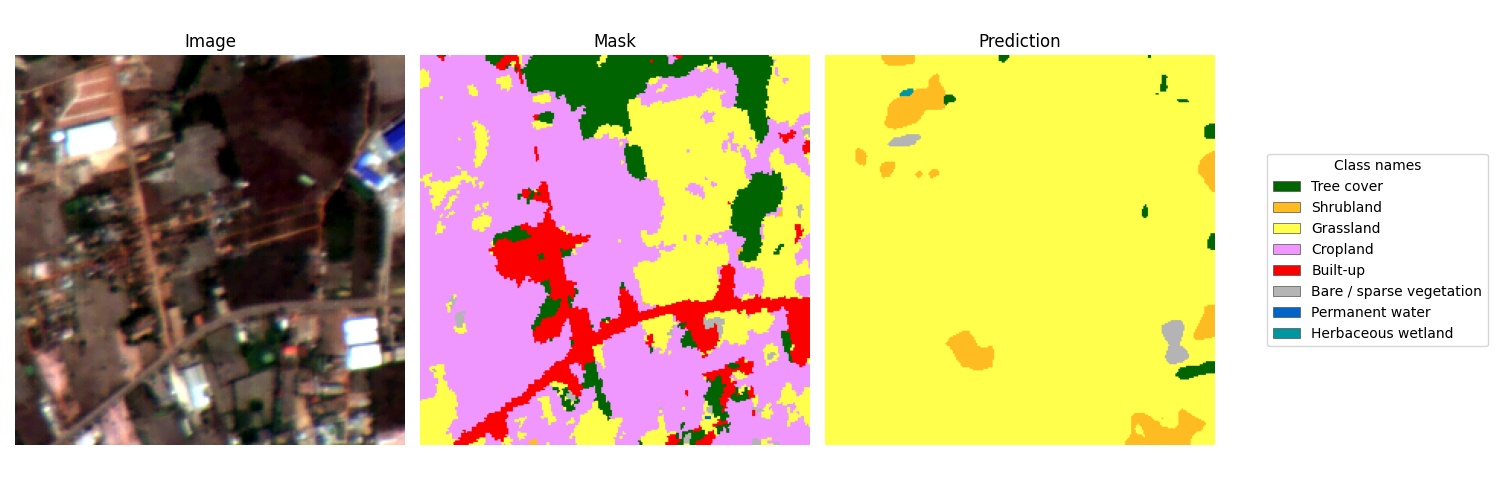
\includegraphics[width=\textwidth]{figures/media_images_samples_4_e83632d014201d2d1873.png}
    \caption[Qualitative Baseline Results]{Sample prediction from real $\Phi$-sat-2 test set of the TerraMind Base model fine-tuned on Sentinel-2.
        The model is unable to generalize to the new sensor and predicts grassland for the entire scene, which is the most common class in the training set. 
    }
    \label{fig:qualitative-baseline}
\end{figure}

\begin{figure}[htbp]
    \centering
    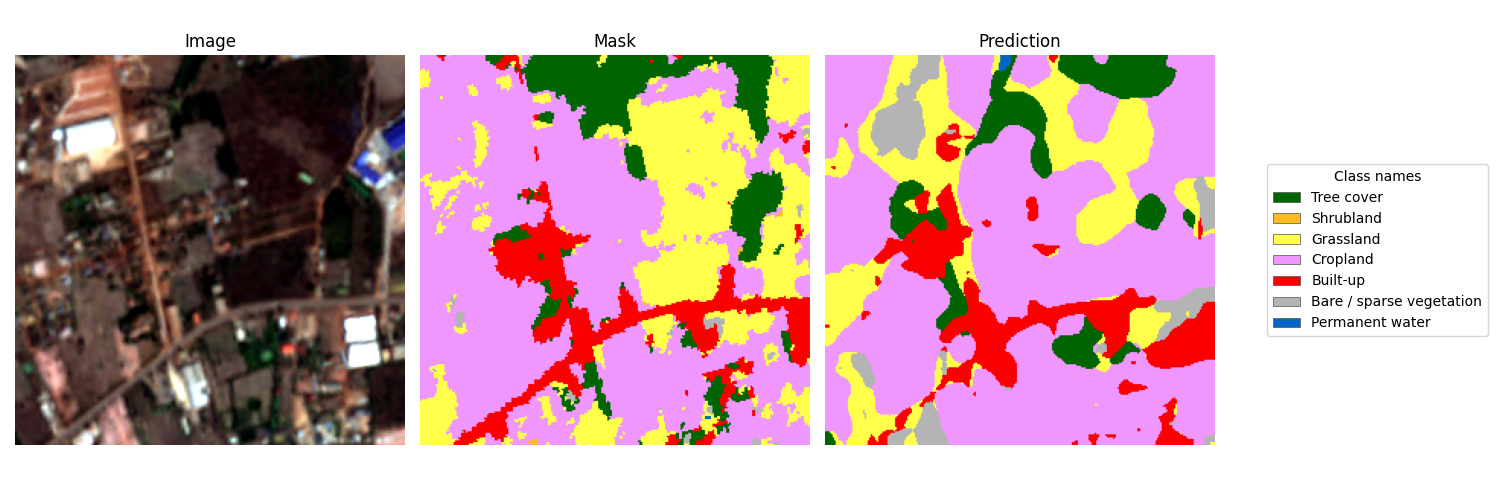
\includegraphics[width=\textwidth]{figures/media_images_samples_4_063cefee1b03274392e7.png}
    \caption[Qualitative Sentinel-2 Results]{Sample prediction from the Sentinel-2 patch of the same scene as of Figure~\ref{fig:qualitative-baseline}, from the TerraMind Base model fine-tuned on Sentinel-2.
        The model is able to correctly predict the classes of the scene, which shows that the poor performance on $\Phi$-sat-2 is not due to a difficult scene or a poor model, but rather to the domain gap between the two sensors.
    }
    \label{fig:qualitative-baseline-s2}
\end{figure}

\bibliographystyle{ieeetr}
\bibliography{references}

\end{document}
